% Modelo de Dissertação do Mestrado em Informática da PUC - Alterado para cumprir a normalização de 2011
%\documentclass[a4paper,brazil,ruledheader,normaltoc,capchap]{abnt}

% Para impressão frente e verso (normalização 2011)g
\documentclass[a4paper,brazil,ruledheader,normaltoc,capchap,twoside,openright]{abnt_pucmg_utf8}

% Não esquecer das alterações no arquivo abnt.cls
% Se estiver usando o Kile no Ubuntu o arquivo fica armazenado em /usr/share/texmf/tex/latex/abntex.
% Comentar a linha 967 
% \vspace*{30pt}% - Linha comentada para reduzir o espaçamento entre o topo da página e o título \chapter
% Alterar a linha 1143
% \vspace*{-30pt} % - Parâmetro alterado de 30pt para -30pt para reduzir o espaçamento entre o top da página e o título do apêndice
% Alterar a linha 985
%\vspace*{-30pt}\par % - Parâmetro alterado de 0pt para -30pt para reduzir o espaçamento entre o top da página e o título \chapter*
% Alterar a linha 991
% Parâmetro alterado de 45pt para 30pt para reduzir o espaçamento entre o texto e o título \chapter*

% Não esquecer das alterações no arquivo acronym.sty
% Se estiver usando o Kile no Ubuntu o arquivo fica armazenado em /usr/share/texmf-texlive/tex/latex/acronym
% Alterar a linha 225
%\item[\protect\AC@hypertarget{#1}{\acsfont{\normalfont{#2}}} --] #3% - Inserir separador entre acrônimo/descrição e remover o negrito com o normalfont
% Pacote para definir explicitamente as margens das páginas
\usepackage[a4paper,inner=3cm,outer=2cm,top=3cm,bottom=2cm]{geometry}

%\usepackage{units}
% Utilize da seguinte forma \unit[78,6]{mA}

% Pacote para gerenciar siglas
\usepackage[printonlyused]{acronym}

% Merge em duas células (linhas diferentes)
\usepackage{multirow}

% Pacote para citação e referências seguindo ABNT no sistema (AUTOR, Data)
%\usepackage[alf, bibjustif,abnt-emphasize=bf]{abntcite}
% MODIFICACAO BY DAVIDYSSON (TROQUEI O COMANDO ABAIXO DE ABNTCITE PARA ABNTEX2CITE)
%\usepackage[alf, abnt-emphasize=em, abnt-thesis-year=title]{abntcite}
\usepackage[alf, abnt-emphasize=em, abnt-thesis-year=title, abnt-etal-text=it]{abntex2cite}
% @article An article from a journal or magazine 
% @inproceedings An article in a conference proceedings
% Força que o tipo de ênfase no nome do simpósio seja em caixa alta
\renewcommand{\emph}{\textsc}

% Pacote para múltiplos arquivos .bib
\usepackage{multibib}
%\newcites{pub}{Refer\^encias das publica\c{c}\~oes}

% Pacote de adequação do formato ABNT para normas da PUCMinas
\usepackage{abnt-PPGInf-PUCMG}

% Pacotes utilitários
\usepackage{graphicx}
%\usepackage{subcaption}

% Pacote para fixar a figura no local desejado
\usepackage{float}

% Pacote para adicionar simbolos as informações de rodapé
\usepackage[symbol]{footmisc}

\usepackage[all]{xy}
%\usepackage[tight]{subfigure}	% Permite a criação de subfiguras
\usepackage{url,amsmath}	% Permite melhorias na codificação de fórmulas
%\usepackage{amsthm}		% Permite melhorias na escrita de teoremas
\usepackage{amssymb}		% Permite utlização de simbolos matemáticos avançados
\usepackage{textcomp}

\usepackage{courier}
\usepackage[portuguese, linesnumbered, ruled, vlined]{algorithm2e}
\usepackage{algorithmic} 	% para algoritmos
\usepackage{listings} 		% para importação de código-fonte
\lstloadlanguages{[Sharp]C,C++,C}
% Alterar o espaçamento da margem no algoritmo
\setlength{\algomargin}{1em}

\usepackage{setspace}

% Pacote para rotação de tabelas/figuras
\usepackage{rotating}

% Pacotes para criação de cronograma/tabela colorida
\usepackage{xcolor,soulutf8}
\usepackage{framed}
\colorlet{shadecolor}{yellow}
\usepackage{array}
\usepackage{longtable}
\usepackage{colortbl}
\usepackage{tabularx}
%\definecolor{lightgray}{gray}{0.9}

\usepackage[official]{eurosym}

\usepackage{paralist}

% Pacote para possibilitar o uso do setboolean para forçar formatos de página diferentes do padrão do documento
\usepackage{ifthen}

\usepackage{chngcntr}
\counterwithout{footnote}{chapter}

% Para inserir captions (nova normalização 2011)
\usepackage[size=normalsize,labelfont=bf,textfont={bf},labelsep=endash]{caption}
\captionsetup[subfloat]{labelfont=bf,textfont={bf}}

% Usado para reduzir espaçamentos entre itens (alíneas, enumerações) com o compactitem
\usepackage{paralist}

% Alterar para sequencial a numeração de figuras e tabelas
\captionsetup{figurewithin=none}
\captionsetup{tablewithin=none}

\setlength{\LTcapwidth}{\textwidth}

% Para o subsubsection aparecer no sumário 
\setcounter{tocdepth}{3}
\setcounter{secnumdepth}{3}

% Para inserir referências via links - não funciona para abntex
%\usepackage[colorlinks=true,pdfstartview=FitV,linkcolor=blue,citecolor=blue,urlcolor=blue,hyperindex,pagebackref=true,pdftex,breaklinks]{hyperref}
%\usepackage[pdftex]{hyperref}
\usepackage{pdfpages}

\usepackage[binary-units = true]{siunitx}
\sisetup{mode=text,range-phrase = {\text{~a~}}}

% Para criar lista de gráficos
\floatstyle{plaintop}
\newfloat{grafico}{H}{loq}
\restylefloat*{grafico}
\floatname{grafico}{Gráfico} 

% Para gerar subfiguras usando o subfloat
\usepackage{subfig}
\newsubfloat[position=top,listofformat=subsimple]{grafico}

% define estilo de posicionamento na caixa
\newsavebox{\leftfig}
\newsavebox{\rightfig}

\newcommand{\csharp}{C\nolinebreak{\bf$^\#$}}
%\renewcommand{\ALG@name}{Algoritmo}
%\renewcommand{\listalgorithmname}{Lista de Algoritmos}

% Configuração de código-fonte
\lstset{%extendedchars=\true, % permite acentos
 %inputencoding=utf8,
 literate=
  {á}{{\'a}}1 {é}{{\'e}}1 {í}{{\'i}}1 {ó}{{\'o}}1 {ú}{{\'u}}1
  {Á}{{\'A}}1 {É}{{\'E}}1 {Í}{{\'I}}1 {Ó}{{\'O}}1 {Ú}{{\'U}}1
  {à}{{\`a}}1 {è}{{\`e}}1 {ì}{{\`i}}1 {ò}{{\`o}}1 {ù}{{\`u}}1
  {À}{{\`A}}1 {È}{{\'E}}1 {Ì}{{\`I}}1 {Ò}{{\`O}}1 {Ù}{{\`U}}1
  {ä}{{\"a}}1 {ë}{{\"e}}1 {ï}{{\"i}}1 {ö}{{\"o}}1 {ü}{{\"u}}1
  {Ä}{{\"A}}1 {Ë}{{\"E}}1 {Ï}{{\"I}}1 {Ö}{{\"O}}1 {Ü}{{\"U}}1
  {â}{{\^a}}1 {ê}{{\^e}}1 {î}{{\^i}}1 {ô}{{\^o}}1 {û}{{\^u}}1
  {Â}{{\^A}}1 {Ê}{{\^E}}1 {Î}{{\^I}}1 {Ô}{{\^O}}1 {Û}{{\^U}}1
  {ã}{{\~a}}1 {Ã}{{\~A}}1 {õ}{{\~o}}1 {Õ}{{\~O}}1
  {œ}{{\oe}}1 {Œ}{{\OE}}1 {æ}{{\ae}}1 {Æ}{{\AE}}1 {ß}{{\ss}}1
  {ç}{{\c c}}1 {Ç}{{\c C}}1 {ø}{{\o}}1 {å}{{\r a}}1 {Å}{{\r A}}1
  {€}{{\EUR}}1 {£}{{\pounds}}1,
 %texcl=true, %codificação dos comentários
 commentstyle=\it\ttfamily, % deixa os comentários em itálico
 stringstyle=\bf\ttfamily, % não lembro o que faz, mas está funcionando
 belowcaptionskip=5pt, % não lembro o que faz, mas está funcionando
 numbers=left, % coloca a numeração na esquerda
 stepnumber=1, % passos da numeração
 firstnumber=1, % primeira linha
 numberstyle=\tiny\ttfamily, % tamanho da fonte da numeração
 breaklines=true, % permitir quebra de linha
 frame=tb, % borda em cima e em baixo
 basicstyle=\footnotesize\ttfamily, % estilo básico
% stringstyle=\ttfamily, % não lembro o que faz, mas está funcionando
 showstringspaces=false, % não mostrar os espaços
 mathescape, % não lembro o que faz, mas está funcionando
 tabsize=3 % tamanho da tabulação
}
\renewcommand{\lstlistingname}{Código}
\renewcommand{\lstlistlistingname}{Lista de Códigos}
\citeoption{abnt-etal-cite=1, abnt-and-type=e}

% the bibtex style generates this command, but it's not defined
% MODIFICACAO BY DAVIDYSSON (DESATIVEI O COMANDO ABAIXO)
%\newcommand{\optionaltextstyle}{}

%%\pdfinfo{%
%%  /Title    (APRIMORAMENTO DE UMA LUVA ELETRÔNICA PARA CAPTURA DOS MOVIMENTOS DA MÃO)
%%  /Author   (Andre Augusto Laudares Ansani)
%%  /Creator  (Andre Augusto Laudares Ansani)
%%  /Producer (Kile - an Integrated LaTeX Environment - %%Version 2.0.85)
%%  /Subject  (Dissertação de Graduação)
%% /Keywords (Palavras chave)
%%}

% PRÉ-TEXTUAIS %%
\begin{document}

% Para forçar que elementos pré-textuais (da capa até o sumário) sejam impressos no anverso da folha
\setboolean{@twoside}{false}

\autor{Andre Augusto Laudares Ansani}

% Coloque o título em caixa alta. É o padrão da PUC.
% Vá no arquivo abnt-PPGInf-PUCMG.sty e procure por esse título (linha 575). Altere para o seu título em caixa alta. Isso será utilizado na folha de aprovação.
\titulo{APRIMORAMENTO DE UMA LUVA ELETRÔNICA PARA CAPTURA DOS MOVIMENTOS DA MÃO}

\orientador[Orientador:]{Prof\textordfeminine. Dr\textordfeminine. Rosilane Ribeiro da Mota}

% Se não tiver, co-orientador, comente a próxima linha.
%\coorientador[Co-orientador:]{Professor}

% Texto
\comentario{Projeto de Monografia apresentada ao Curso de Engenharia de Computação da 
Pontifícia Universidade Católica de Minas Gerais, como requisito parcial para obtenção do título de Bacharel em Engenharia de Computação.}


% Instituição
\instituicao{Mestrado em Informática \par Instituto de Informática \par Pontifícia Universidade Católica de Minas Gerais}

% Local
\local{Belo Horizonte}

% Data
\data{\the\year}
\capa

%Para forçar que a ficha catalográfica seja impressa no verso da folha de aprovação
%\setboolean{@twoside}{true}

% Gera a folha de rosto
\folhaderosto

% Ficha catalográfica
%% Ficha catalográfica
% INCLUIR O ARQUIVO PDF GERADO PELA BIBLIOTECA COMO FIGURA.
\begin{figure}[h!]
	\vspace*{-3.3cm}
	\hspace*{-3cm}
%	% Suponha o nome do arquivo em pre-texto/ficha-catalografica/fichacatalografica.pdf
	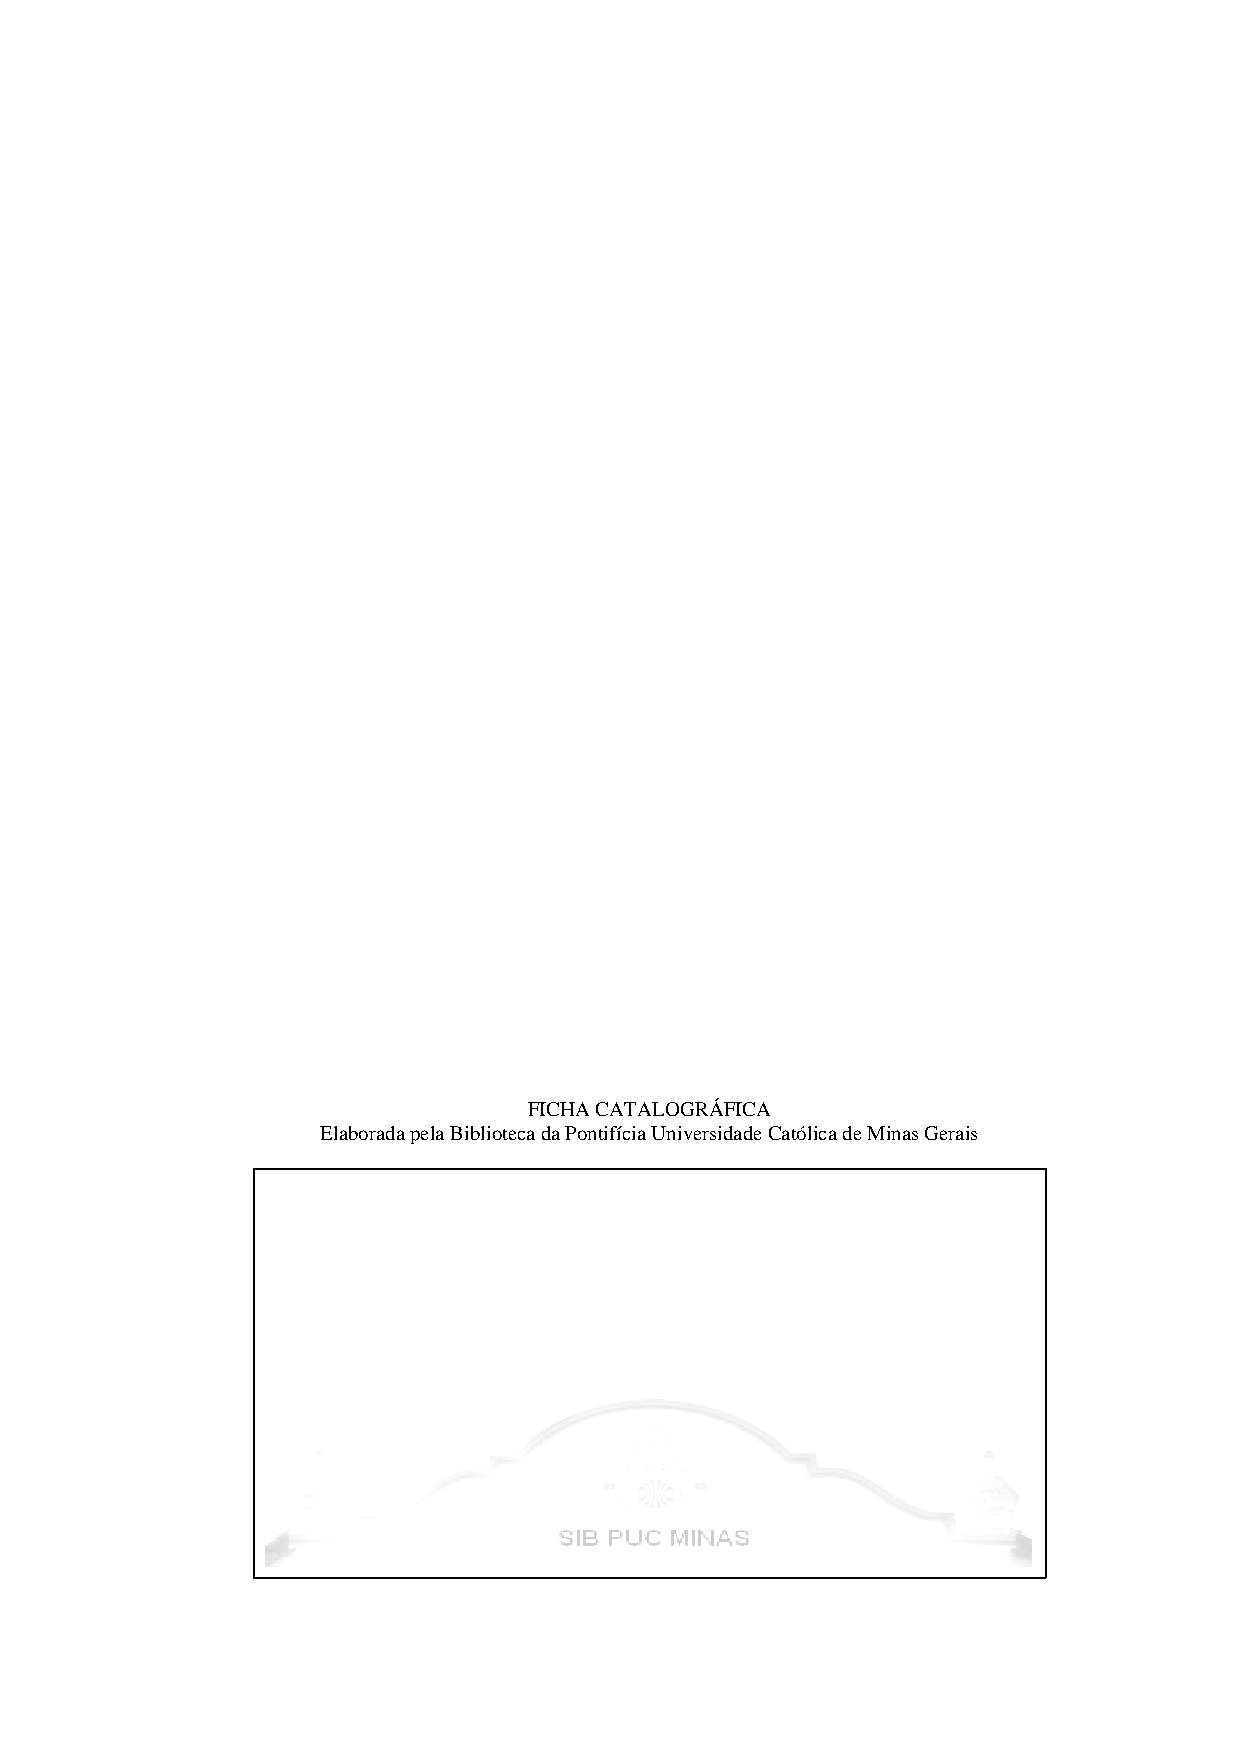
\includegraphics[width=\textwidth]{pre-texto/ficha-catalografica} 
	\newpage
\end{figure}
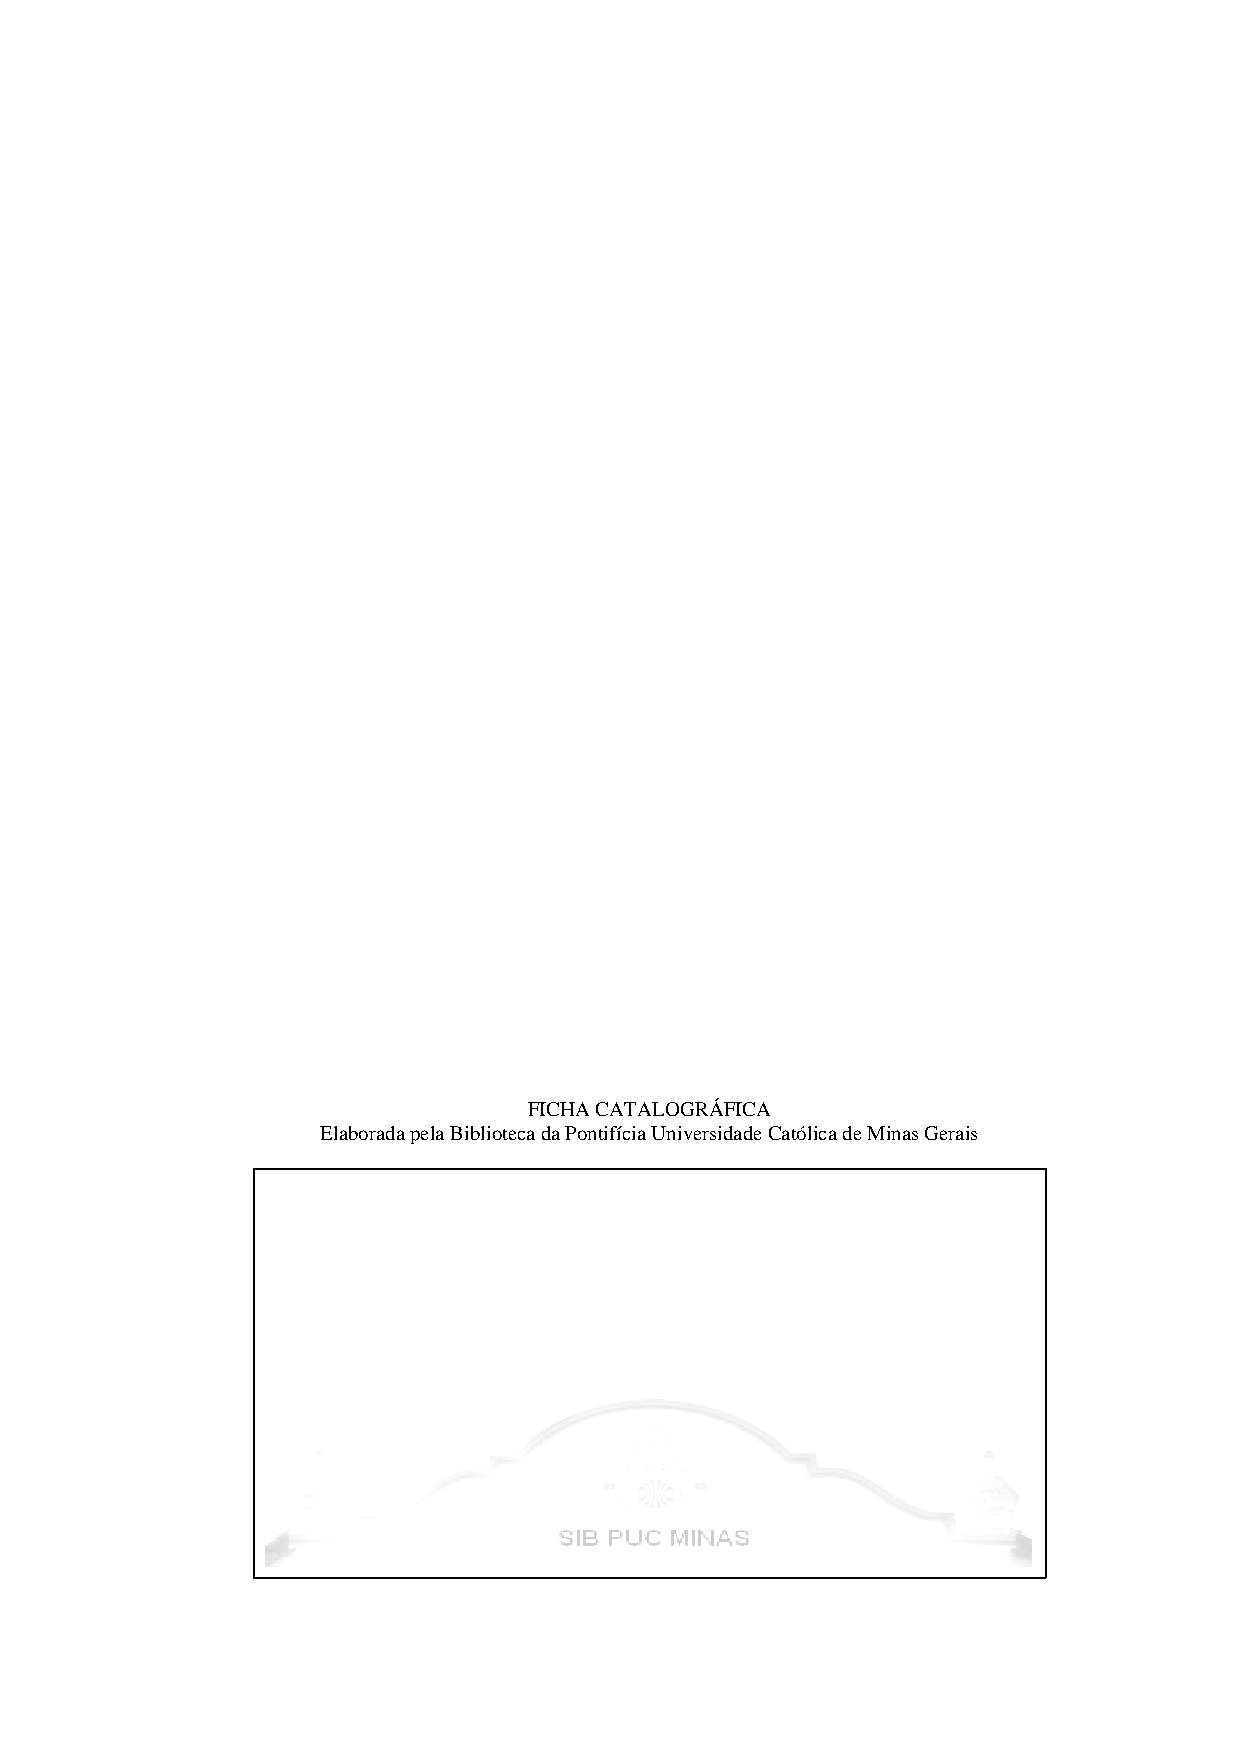
\includepdf[pages={1}]{pre-texto/ficha-catalografica.pdf}

% Para forçar que elementos pré-textuais (da capa até o sumário) sejam impressos no anverso da folha
%\setboolean{@twoside}{false}

% Folha de aprovação
% Termo de Aprovação

% Texto da aprovação
\textoaprovacao{Dissertação apresentada ao Curso de Engenharia de Computação como requisito parcial para obtenção do título de Bacharel pela Pontifícia Universidade Católica de Minas Gerais.}

% Primeira assinatura
\primeiroassina{Prof\textordfeminine. Dr\textordfeminine. Rosilane Ribeiro da Mota -- PUC Minas}

% Segunda assinatura
\segundoassina{Prof. Dr. Zenilton Kleber Gonçalves do
Patrocínio Júnior -- PUC Minas}

% Terceira assinatura
%\terceiroassina{Prof. Dr. Membro externo -- Instituicao}

% Quarta assinatura
%\quartoassina{}

% Data da defesa
\localdia{Belo Horizonte, \today}

% Gera o termo de aprovação
\termodeaprovacao	

% Dedicatória
%% Dedicatória
\newpage

% Espaçamento do topo da página até o texto da dedicatória
\vspace*{22cm}

% Espaçamento na esqueda
\hspace{8cm}\begin{minipage}{.60\textwidth}
            \textit{Texto da dedicatoria (opcional)}
            \end{minipage}

% Agradecimentos
% Agradecimentos
%\chapter*{Agradecimentos}
\begin{center}
	\normalsize
	\textbf{AGRADECIMENTOS}
\end{center}

\textit{Aos meus pais pelo incentivo e apoio incondicional.}
  
\textit{À minha orientadora, Rosilane Mota, pela orientação, apoio e confiança.}
  
\textit{À Pontifícia Universidade Católica de Minas Gerais e seu corpo docente, pelos ensinamentos e oportunidades oferecidas.}

\textit{E a todos que direta ou indiretamente fizeram parte da minha formação, o meu muito obrigado.}

% Epígrafe
% Epígrafe
\newpage

% Espaçamento entre topo da página e texto da epígrafe
\vspace*{10cm}
% Espaçamento na esqueda
\hspace{4cm}\begin{minipage}{.51\textwidth}

% Texto da epígrafe
\textit{``Se vi mais longe foi por estar de pé sobre ombros de Gigantes.'' }

%Nome do autor
\begin{flushright}\itshape Isaac Newton \upshape\end{flushright}

\end{minipage}

% Resumo
% Resumo
\begin{resumo}
% Diminuir espaçamento entre título e texto
\vspace{-1cm}

% Texto do resumo: sem paragrafo, justificado, com espaçamento 1,5 cm
\onehalfspacing
\noindent 
%\begin{shaded*}
Dispositivos de \ac{IHC} estão cada vez mais presentes em nosso cotidiano, com telas de toque ou controles por gestos, permitindo uma utilização mais natural e intuitiva de \textit{Hardware} e \textit{Software}. Luvas Eletrônicas são um tipo de dispositivo \ac{IHC} que permite o controle de braços robóticos ou objetos em ambientes virtuais através de gestos da mão do usuário, porém são muito caras e isso torna seu uso inviável para aplicações não profissionais. Este trabalho apresenta a continuação do desenvolvimento de um protótipo de luva eletrônica elaborado por \citeonline{roversi}, utilizando-se a plataforma \textit{Arduino}, sensores de flexão e a \ac{IMU} \textit{MPU-9250}. As melhorias propostas são incluir a capacidade de detecção de movimentos de adução e abdução dos dedos e desvios radial e ulnar do pulso, além de reduzir o ruído proveniente da \ac{IMU} e dos sensores de flexão. Os movimentos do usuário serão mostrados na tela do computador através de um modelo \ac{3D} de uma mão humana utilizando a plataforma \textit{Unity} de desenvolvimento, de modo a verificar a correção dos dados capturados e enviados. A solução para a adição dos movimentos dos dedos foi limitada, não permitindo a movimentação do dedo médio. A solução para detecção dos movimentos do pulso foi satisfatória e exibe boa precisão. Os filtros aplicados nos sensores foram satisfatórios provendo boa redução de ruídos sem comprometer a responsividade dos movimentos.

%\end{shaded*}
% Espaçamento para as palavras-chave
\vspace*{.75cm}

% Palavras-chave: sem parágrafo, alinhado à esquerda
\noindent Palavras-chave: interação humano computador. luva eletrônica. arduino. unity. acelerômetro. giroscópio. magnetômetro. IMU. sensor flexão.\\
% Segunda linha de palavras-chave, com espaçamento.
%\indent\hspace{2cm}Palavra.

\end{resumo}

% Abstract
% Abstract
\begin{abstract}
% Diminuir espaçamento entre título e texto
\vspace{-1cm}
% Texto do resumo, em inglês: sem paragrafo, justificado, com espaçamento 1,5 cm
\onehalfspacing
\noindent
Human-Computer Interaction devices are increasingly present in our daily lives, with touchscreens or gesture controls, allowing more natural and intuitive use of \textit {Hardware} and \textit {Software}. Data Gloves are a type of Human-Computer Interaction device that allows control of robotic arms or objects in virtual environments through hand gestures, but they are expensive and this makes their use unfeasible for non-professional applications. This work presents the further development of an data glove prototype made by \citeonline{roversi}, using the \textit{Arduino} platform, felxibility sensors and the \ac{IMU} \textit{MPU-9250}. We propose to include the ability to detect adduction and abduction movements of the fingers and radial and ulnar deviations of the wrist, in addition to reducing the noise coming from the \ac{IMU} and the flex sensors. User movements will be shown on the computer screen through a \ac{3D} model of a human hand using the \textit{Unity} development platform. The solution for the addition of finger movements was limited, not allowing movement of the middle finger. The solution for detecting wrist movements was satisfactory and shows good accuracy. The filters applied to the sensors were satisfactory providing good noise reduction without compromising the responsiveness of the movements.

% Espaçamento para as palavras-chave
\vspace*{.75cm}

% Palavras-chave: sem parágrafo, alinhado à esquerda
\noindent Keywords: human computer interaction. data glove. arduino. unity. accelerometer. gyroscope. magnetometer. IMU. flex sensor.\\
% Segunda linha de palavras-chave, com espaçamento.
%\indent\hspace{1.4cm} Keyword.

\end{abstract}

\makeatletter
\renewcommand\numberline[1]{
	\leftskip 0em
	\rightskip 1.6em
	\parfillskip -\rightskip
	\parindent 0em
	\@tempdima 2.0em
	\vspace{0em} \advance\leftskip \@tempdima \null\nobreak\hskip -\leftskip
	FIGURA \normalfont #1 -- }
\makeatother

% Lista de figuras
\listoffigures

\makeatletter
\renewcommand\numberline[1]{
	\leftskip 0em
	\rightskip 1.6em
	\parfillskip -\rightskip
	\parindent 0em
	\@tempdima 2.0em
	\vspace{0em} \advance\leftskip \@tempdima \null\nobreak\hskip -\leftskip
	TABELA \normalfont #1 -- }
\makeatother

%Lista de tabelas
\listoftables

\makeatletter
\renewcommand\numberline[1]{
	\leftskip 0em
	\rightskip 1.6em
	\parfillskip -\rightskip
	\parindent 0em
	\@tempdima 2.0em
	\vspace{0.5em} \advance\leftskip \@tempdima \null\nobreak\hskip -\leftskip
	GRÁFICO \normalfont #1 -- }
\makeatother

%Lista de graficos
\listof{grafico}{Lista de Gráficos}

% Lista de siglas
% Lista de Abreviaturas e Siglas
%\chapter*{Lista de Abreviaturas e Siglas}
\chapter*{Lista de Abreviaturas e Siglas}

% Mantenha sempre em ordem alfabética.

\begin{acronym}
\acro{3D} {\textit{Tridimensional}}
\acro{A/D} {\textit{Analógico/Digital}}
\acro{DOF} {\textit{Degrees Of Freedom}}
\acro{DMA} {\textit{Desvio Médio Absoluto}}
\acro{DMP} {\textit{Digital Motion Processor\texttrademark}}
\acro{DP} {\textit{Desvio Padrão}}
\acro{FIFO} {\textit{First In First Out}}
\acro{GND} {\textit{Ground}}
\acro{I2C} {\textit{Inter-Integrated Circuit}}
\acro{IF} {\textit{Interfalangiana}}
\acro{IFD} {\textit{Interfalangiana Distal}}
\acro{IFP} {\textit{Interfalangiana Proximal}}
\acro{IHC} {\textit{Interação Humano-Computador}}
\acro{IMU} {\textit{Inertial Measurement Unit}}
\acro{IMMU} {\textit{Inertial and Magetic Measurement Units}}
\acro{INT} {\textit{Interrupt}}
\acro{MCF} {\textit{Metacarpofalangiana}}
\acro{RA} {\textit{Realidade Aumentada}}
\acro{RSR} {\textit{Relação Sinal-Ruído}}
\acro{RV} {\textit{Realidade Virtual}}
\acro{SCL} {\textit{Serial Clock}}
\acro{SDA} {\textit{Serial Data}}
\acro{USB} {\textit{Universal Serial Bus}}
\end{acronym}

\makeatletter
\renewcommand\numberline[1]{#1\hspace{0.8em}}
\makeatother

% Altera para espaçamento simples a partir daqui
\singlespacing

% Sumário
\tableofcontents

% Altera para espaçamento 1,5 a partir daqui
\onehalfspacing

%% TEXTUAIS 
% Para forçar que elementos textuais e pós-textuais sejam impressos no anverso e verso das folhas
%\setboolean{@twoside}{true}
% Altere o número da página para o correto. Conte todas as páginas frente e verso, menos a capa, inclusive a ficha catalográfica até a página do primeiro capítulo.
\setcounter{page}{23}

% Capítulos
% Para forçar que o capítulo de introdução comece no anverso
\setboolean{@openright}{true}
% Nome do capítulo
\chapter{Introdução}
\label{ch:intro}
% Diminuir espaçamento entre título e texto
\vspace{-1.9cm}
% Texto do capítulo

Pesquisas na área de \acf{IHC} tem sido realizadas desde a década de 1960 \cite{myers1998brief}. Hoje interage-se com dispositivos eletrônicos utilizando teclados, \textit{mouses}, acelerômetros e giroscópios, porém, com a popularização de tecnologias de realidade virtual, realidade aumentada e hologramas, foi necessária a criação de novos métodos de \ac{IHC} para que a interação com estes ambientes seja feita de maneira natural e intuitiva para seres humanos. Um dos dispositivos desenvolvidos para esse fim são as luvas eletrônicas que capturam os movimentos dos dedos e posição da mão do usuário através de sensores e os reproduzem em um ambiente tridimensional ou em algum atuador robótico.

A captura dos dados em tempo real é bastante complexa devido à grande variedade de posições que podem ser realizadas e número de variáveis a serem monitoradas, o que requer alto poder computacional. Atualmente exitem alguns dispositivos que atingem esses objetivos, como a \textit{CyberGlove III} que é uma luva eletrônica com até 22 sensores e comunicação sem fio. Outras variedades de luvas eletrônicas como a \textit{Manus VR} ou \textit{Avatar VR} são projetadas para experiências com \acf{RV} e, por isso, utilizam tecnologias baseadas em câmeras ou sensores de infravermelho posicionados no ambiente ao redor do usuário para captar os movimentos. O problema é o alto custo destes dispositivos, variando de US\$250,00 até US\$12.995,00, o que dificulta seu acesso, tanto para fins de pesquisa, quanto para sua utilização prática.

Este trabalho baseia-se no protótipo de uma luva eletrônica de baixo custo desenvolvido por \citeonline{roversi} utilizando a plataforma \textit{Arduino} para aquisição de dados de sensores de flexibilidade e de giroscópios para o controle de uma mão \acf{3D} modelada na plataforma \textit{Unity}. O protótipo desenvolvido possui algumas limitações, não sendo possível detectar movimentos de adução e abdução dos dedos e de desvios radial e ulnar do pulso (Figura \ref{fig:movimentos}), e ainda capta muitos ruídos provenientes do acelerômetro fazendo o modelo virtual da mão oscilar de modo não satisfatório. Este trabalho apresenta um novo protótipo de uma luva eletrônica que capta os movimentos de adução e abdução dos dedos e desvio radial e ulnar do pulso, fazendo uso de duas \textit{Unidades de Medição Inercial} (IMU) e 14 sensores de flexão. Filtros foram aplicados para a suavização das leituras com resultados satisfatórios.

\section{Objetivo Geral}
\label{sec:objg}
O objetivo geral desse trabalho é evoluir o protótipo da luva eletrônica para captura de movimentos de \citeonline{roversi}, com o intuito de incluir os movimentos de adução e abdução dos dedos e desvio radial e ulnar do pulso, reduzir os ruídos captados através de um filtro e melhorar a fixação dos sensores.

\begin{figure}[ht]
% Alterar espaçamentos antes e depois do caption
\setlength{\abovecaptionskip}{0pt}
\setlength{\belowcaptionskip}{0pt}
% Caption
\caption[Movimentos da mão]{Movimentos da mão}
\centering
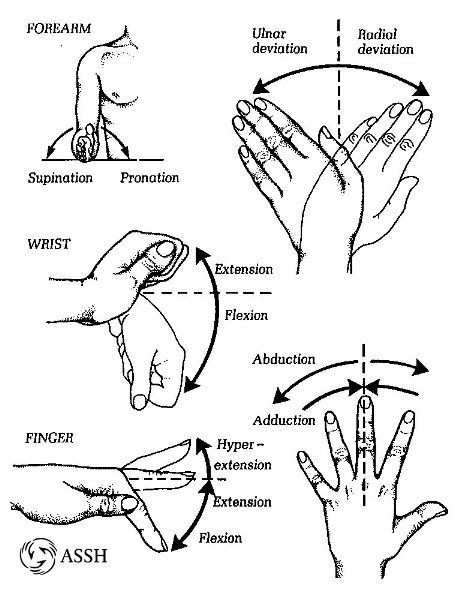
\includegraphics[width=.5\textwidth]{imagem/movimentos}
% Caption centralizada
\captionsetup{justification=centering}
\captionfont{\small{\textbf{\\Fonte: \citeonline{movimentos}}}}	
\label{fig:movimentos}
\end{figure}

\section{Objetivos Específicos}
\label{sec:obje}
Os objetivos específicos deste trabalho consistem em:
  
\begin{compactitem}
	\item[a)] desenvolver um método para captura dos movimentos de adução e abdução dos dedos;
	\item[b)] desenvolver um método para captura dos movimentos de desvios radial e ulnar do pulso;
	\item[c)] aplicar filtros para redução de ruídos dos sensores;
    \item[d)] comparar os resultados com o protótipo de \citeonline{roversi}.
\end{compactitem}

\section{Justificativa}
\label{sec:jus}
Luvas eletrônicas podem ser utilizadas em uma variedade de aplicações. Um caso de uso seria o de médicos que realizam cirurgias e precisam retirar suas luvas para utilizar telas sensíveis ao toque para visualizar informações do paciente. Tais médicos poderiam utilizar luvas eletrônicas para interagir com computadores através de gestos, reduzindo o contato com outros objetos na sala de cirurgia e diminuindo o risco de contaminações. Além disso tais luvas podem ser utilizadas para controle remoto de operadores terminais robóticos, imersão do usuário em um ambiente de \ac{RV} ou reconhecimento de linguagem de sinais. Em cada uma desas aplicações espera-se que os movimentos realizados pelo usuário sejam reproduzidos com fidelidade e precisão, para que a tarefa a ser realizada seja concluída com eficiência.


\section{Organização do Trabalho}
\label{sec:org}
Este trabalho está organizado como segue. O Capítulo \ref{ch:revisao} apresenta tecnologias já existentes e forma a base teórica da pesquisa realizada. A Seção \ref{sec:brac} apresenta um estudo sobre diferentes braços e mãos robóticas. A Seção \ref{sec:luv} apresenta uma comparação entre algumas luvas existentes no mercado. A Seção \ref{sec:sens} mostra os tipos de sensores que podem ser utilizados na construção de luvas eletrônicas. A Seção \ref{sec:trabrel} mostra trabalhos relacionados com o tema proposto. O Capítulo \ref{ch:meto} descreve a solução elaborada para o problema proposto com os requisitos descritos na Seção \ref{sec:requisitos}, os componentes utilizados na Seção \ref{sec:hardware} e os \textit{softwares} utilizados na Seção \ref{sec:software}. O Capítulo \ref{ch:desenvolvimento} apresenta detalhes do desenvolvimento do trabalho, descrevendo o \textit{hardware} na Seção \ref{sec:met_software} e o \textit{software} na Seção \ref{sec:met_software}. No Capítulo \ref{ch:resultados} são apresentadas as análises dos resultados e, por fim, o Capítulo \ref{ch:conclusao} mostra as conclusões e possíveis trabalhos futuros.
% Os demais capítulos não precisam começar no anverso
\setboolean{@openright}{false}
% Nome do capítulo
\chapter{Revisão de Literatura}
% Label para referenciar
\label{ch:revisao}

% Diminuir espaçamento entre título e texto
\vspace{-1.9cm}

% Texto do capítulo
Este capítulo apresenta uma visão geral das técnicas e tecnologias existentes que se relacionam com o tema do trabalho proposto. Foi feita uma pesquisa sobre braços e mãos robóticas, suas aplicações e tecnologias utilizadas, além de um estudo sobre luvas eletrônicas e sensores comumente adotados para seu funcionamento. Os trabalhos citados, e outros trabalhos relacionados, podem ser encontrados na Biblioteca Digital IEEE Xplore (\citeonline{ieee}) buscando pelos termos \textit{``robot arm''}, \textit{``data glove''} ou similares.

\section{Braços Robóticos}
\label{sec:brac}
Braços robóticos são máquinas programáveis compostas por articulações, construídas para a realização de tarefas repetitivas, desagradáveis ou perigosas \cite{occupational1996osha}. Possuem articulações análogas às existentes nos braços humanos, como ombros, cotovelos e pulsos. O atuador robótico (\textit{end effector}, em inglês) é a parte do robô, geralmente conectada ao pulso, que interage com o ambiente e seria equivalente à mão humana \cite{end_effect}. Outra característica importante dos braços robóticos é a quantidade de Graus de Liberdade (\ac{DOF}), ou seja, a quantidade de parâmetros independentes necessários para determinar a posição final do atuador. Nos próximos parágrafos serão apresentados trabalhos envolvendo braços robóticos, com o intuito de apresentar uma visão geral das tecnologias e técnicas utilizadas.

Existem aplicações comuns de braços robóticos para pintura, soldagem, rotação e transporte de peças. Os braços robóticos mais comuns utilizam garras como atuadores, pois são fáceis de fabricar e controlar, porém, isso limita a quantidade de movimentos que o robô pode realizar. Em certas aplicações, como na fabricação de próteses robóticas, é desejável que se tenha uma maior quantidade de \ac{DOF} no atuador para garantir maior similaridade com a mão humana.

De acordo com \citeonline{potkonjak1998redundancy}, o conjunto de mão e braço possui no total 26 \ac{DOF} (7 para o braço e 19 para a mão). Para a tarefa de escrita com um lápis, por exemplo, pode-se reduzir os \ac{DOF} da mão e do braço para 2 e 6, respectivamente, totalizando um mínimo de 8 \ac{DOF}, representados na Figura \ref{fig:dof}. O trabalho dos autores se foca em analisar o movimento de um braço antropomórfico na tarefa de escrita, elaborando um novo esquema de controle. Foi que para um certo nível de legibilidade, existe uma inclinação ideal das letras que resulta em um movimento mínimo dos dedos.

\begin{figure}[h]
  % Alterar espaçamentos antes e depois do caption
  \setlength{\abovecaptionskip}{0pt}
  \setlength{\belowcaptionskip}{0pt}
  % Caption
  \caption[Modelo de articulações do braço e mão]{Modelo de articulações do braço e mão}
  \centering
  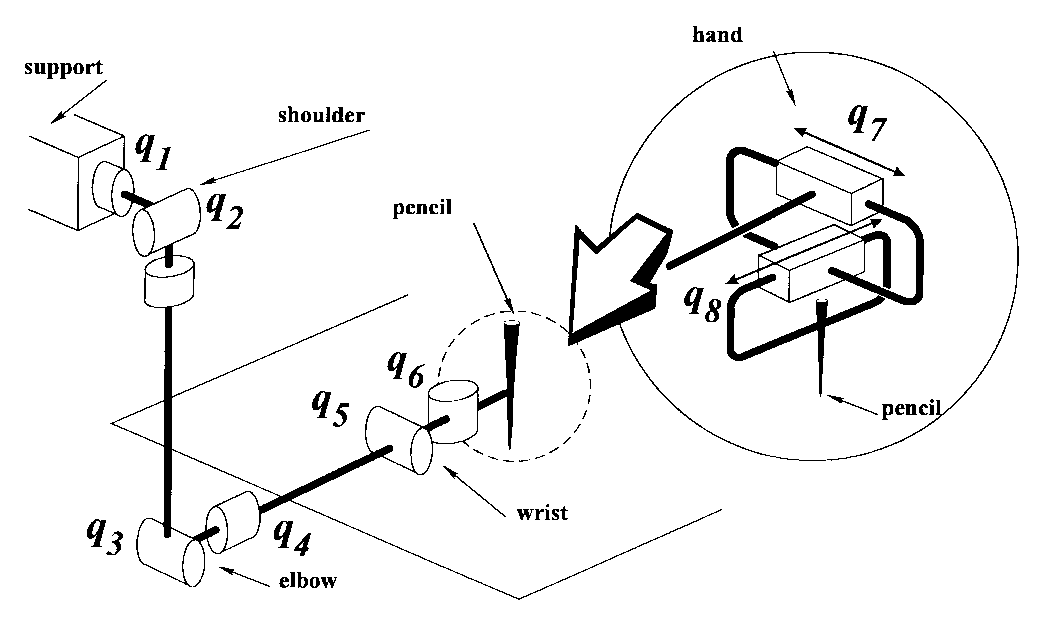
\includegraphics[width=.5\textwidth]{imagem/redundancy_dof}
  % Caption centralizada
  \captionsetup{justification=centering}
  \captionfont{\small{\textbf{\\Fonte: \citeonline{potkonjak1998redundancy}}}}
  \label{fig:dof}
\end{figure}

O trabalho realizado por \citeonline{sun2013calligraphy} descreve um robô com 6 \ac{DOF} denominado \textit{Callibot} (Figura \ref{fig:callibot}), capaz de escrever caracteres chineses utilizando um pincel. Os caracteres são ``ensinados'' gravando as posições de cada motor periodicamente enquanto uma pessoa escreve com o pincel e, em seguida, o robô reproduz os movimentos gravados. Os resultados obtidos foram satisfatórios, mostrando que \textit{Callibot} consegue reproduzir trabalhos complexos com estética agradável.

\begin{figure}[H]
  \setlength{\abovecaptionskip}{0pt}
  \setlength{\belowcaptionskip}{0pt}
  \caption[Callibot]{Callibot}
  \centering
  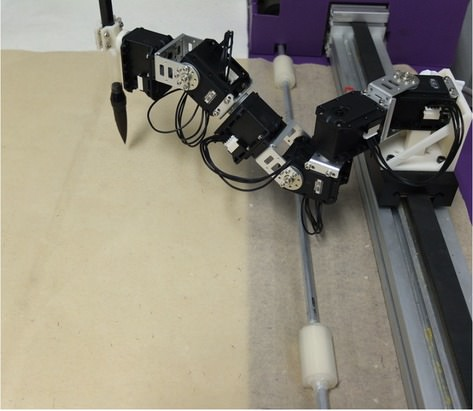
\includegraphics[width=.5\textwidth]{imagem/callibot}
  \captionsetup{justification=centering}
  \captionfont{\small{\textbf{\\Fonte: \citeonline{sun2013calligraphy}}}}
  \label{fig:callibot}
\end{figure}

O trabalho de \citeonline{xudesign} mostra o desenvolvimento de uma mão robótica, mostrada no Figura \ref{fig:antro_hand}, que tenta replicar partes biomecânicas importantes da mão, fazendo com que ela seja um réplica que possui características cinemáticas e dinâmicas similares. Os autores propõem que essa mão robótica possa ser utilizada para aplicações de manipulação remota de objetos, e possa ser integrada com sensores de toque na ponta dos dedos, além do poder servir como base para regeneração de membros e para pesquisas na área de neuroprostética\footnote{Área de pesquisa para desenvolvimento de próteses neurais. Uma prótese neural é um dispositivo que fornece ou recebe informações do sistema nervoso \cite{neuro}.}.

\begin{figure}[H]
  \setlength{\abovecaptionskip}{0pt}
  \setlength{\belowcaptionskip}{0pt}
  \caption[Mão antropomórfica]{Mão antropomórfica}
  \centering
  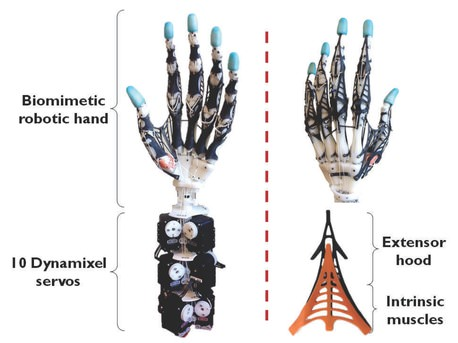
\includegraphics[width=.5\textwidth]{imagem/antro_hand}
  \captionsetup{justification=centering}
  \captionfont{\small{\textbf{\\Fonte: \citeonline{xudesign}}}}
  \label{fig:antro_hand}
\end{figure}

Em \citeonline{konnaris2016ethohand}, também foi desenvolvida uma mão robótica chamada de \textit{EthoHand} (Figura \ref{fig:etho_hand}). O dispositivo possui 24 \ac{DOF} e com articulação esférica no polegar, possibilitando movimentos naturais mais complexos para manipulação de objetos. A articulação funciona a partir de tendões conectados ao polegar e atuados por servomotores localizados externamente.

\begin{figure}[H]
  \setlength{\abovecaptionskip}{0pt}
  \setlength{\belowcaptionskip}{0pt}
  \caption[Detalhe da articulação esférica da EthoHand]{Detalhe da articulação esférica da EthoHand}
  \centering
  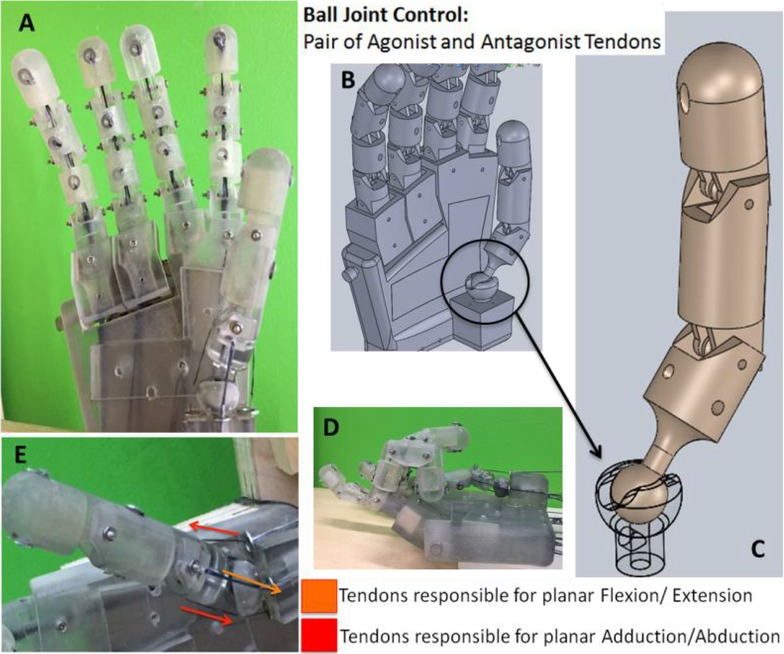
\includegraphics[width=.5\textwidth]{imagem/etho_hand}
  \captionsetup{justification=centering}
  \captionfont{\small{\textbf{\\Fonte: \citeonline{konnaris2016ethohand}}}}
  \label{fig:etho_hand}
\end{figure}

O trabalho de \citeonline{liu2008multisensory} apresenta uma mão robótica chamada de DLR/HIT HAND II (Figura \ref{fig:dex_hand}), com 5 dedos que possui sensores de posição, temperatura e força. Enquanto os outros trabalhos apresentados nessa seção utilizam motores externos que controlam tendões que movimentam os dedos, essa mão robótica utiliza motores e componentes eletrônicos que ficam no interior de cada dedo e da palma da mão para movimentá-los, tornando o produto final mais compacto e portável.

\begin{figure}[H]
  \setlength{\abovecaptionskip}{0pt}
  \setlength{\belowcaptionskip}{0pt}
  \caption[DLR/HIT HAND I e II]{DLR/HIT HAND I e II}
  \centering
  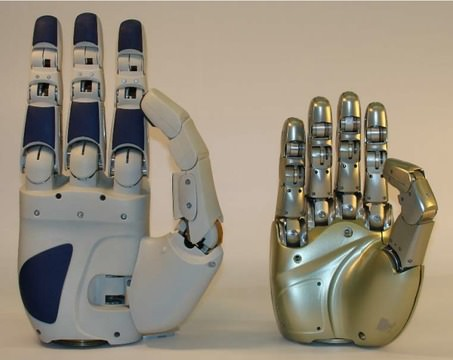
\includegraphics[width=.5\textwidth]{imagem/dex_hand}
  \captionsetup{justification=centering}
  \captionfont{\small{\textbf{\\Fonte: \citeonline{liu2008multisensory}}}}
  \label{fig:dex_hand}
\end{figure}

Para o controle de braços e mãos robóticas, principalmente as mais antropomórficas, é comum a utilização de luvas eletrônicas, como no trabalho de \citeonline{konnaris2016ethohand}, onde foi utilizada a \textit{CyberGlove} para controle remoto da mão robótica desenvolvida. Luvas eletrônicas são úteis pois possibilitam a replicação mais fiel de movimentos humanos além de permitir um controle mais intuitivo ao usuário.

\section{Luvas Eletrônicas (\textit{Data Gloves})}
\label{sec:luv}
Luvas eletrônicas (\textit{Data Gloves}) são dispositivos que utilizam sensores de movimento, como acelerômetros, giroscópios ou sensores de flexibilidade, para reconhecimento ou reprodução de gestos da mão humana \cite{kim20093}. Elas são utilizadas para, por exemplo, captura de movimentos das mãos para utilização em filmes, jogos digitais, reconhecimento de linguagem de sinais, controle de atuadores robóticos ou para \ac{IHC} e interação com ambientes de \ac{RV}.

De acordo com \citeonline{sturman1994survey}, a primeira luva eletrônica, a \textit{Sayre Glove} (Figura \ref{fig:sayre}) foi desenvolvida por Thomas DeFanti e Daniel Sandin na Universidade de Illinois em Chicago em 1976. Ela funcionava com tubos flexíveis que possuíam um emissor e um receptor de luz posicionados sobre os dedos e, conforme se flexionava, a quantidade de luz no receptor variava, gerando uma diferença de tensão que era medida e então usada como entrada para algum sistema. Na indústria do entretenimento, ainda segundo os autores, a fabricante de brinquedos \textit{Mattel} produziu em 1989 uma luva eletrônica de baixo custo chamada \textit{Power Glove}, que era usada como controle para alguns jogos da plataforma \textit{Nintendo}. Seu produto utilizava uma tinta resistiva que registrava o flexionamento dos dedos e um sensor acústico que captava a posição da mão no espaço com o auxílio de um emissor acústico instalado sobre a televisão. A tecnologia utilizada em luvas eletrônicas evoluiu bastante, contando com sensores mais precisos, novas técnicas de de captação de movimentos utilizando sensores de campo magnético \cite{fahn2005development} ou acelerômetros \cite{kim20093} e de cálculo de posicionamento no espaço utilizando sensores de luz infravermelha ou câmeras. A luva proposta nesse trabalho apresenta uma solução de baixo custo para captura de movimentos dos dedos e do pulso.

\begin{figure}[h]
  \setlength{\abovecaptionskip}{0pt}
  \setlength{\belowcaptionskip}{0pt}
  \caption[Sayre Glove]{Sayre Glove}
  \centering
  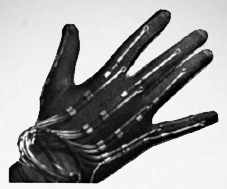
\includegraphics[width=.4\textwidth]{imagem/sayreGlove}
  \captionsetup{justification=centering}
  \captionfont{\small{\textbf{\\Fonte: \citeonline{sayre}}}}
  \label{fig:sayre}
\end{figure}

\begin{figure}[ht!]
  \centering
  % Alterar espaçamentos antes e depois do caption
  \setlength{\abovecaptionskip}{0pt}
  \setlength{\belowcaptionskip}{0pt}
  % Caption
  \caption[Exemplos de luvas eletrônicas]{Exemplos de luvas eletrônicas}
  \subfloat[5DT Data Glove Ultra]{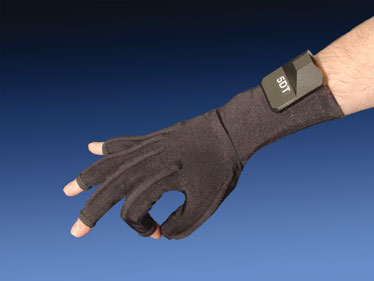
\includegraphics[height= 5cm]{imagem/5dtultra}\label{fig:5dt}}
  \quad
  \subfloat[Avatar VR]{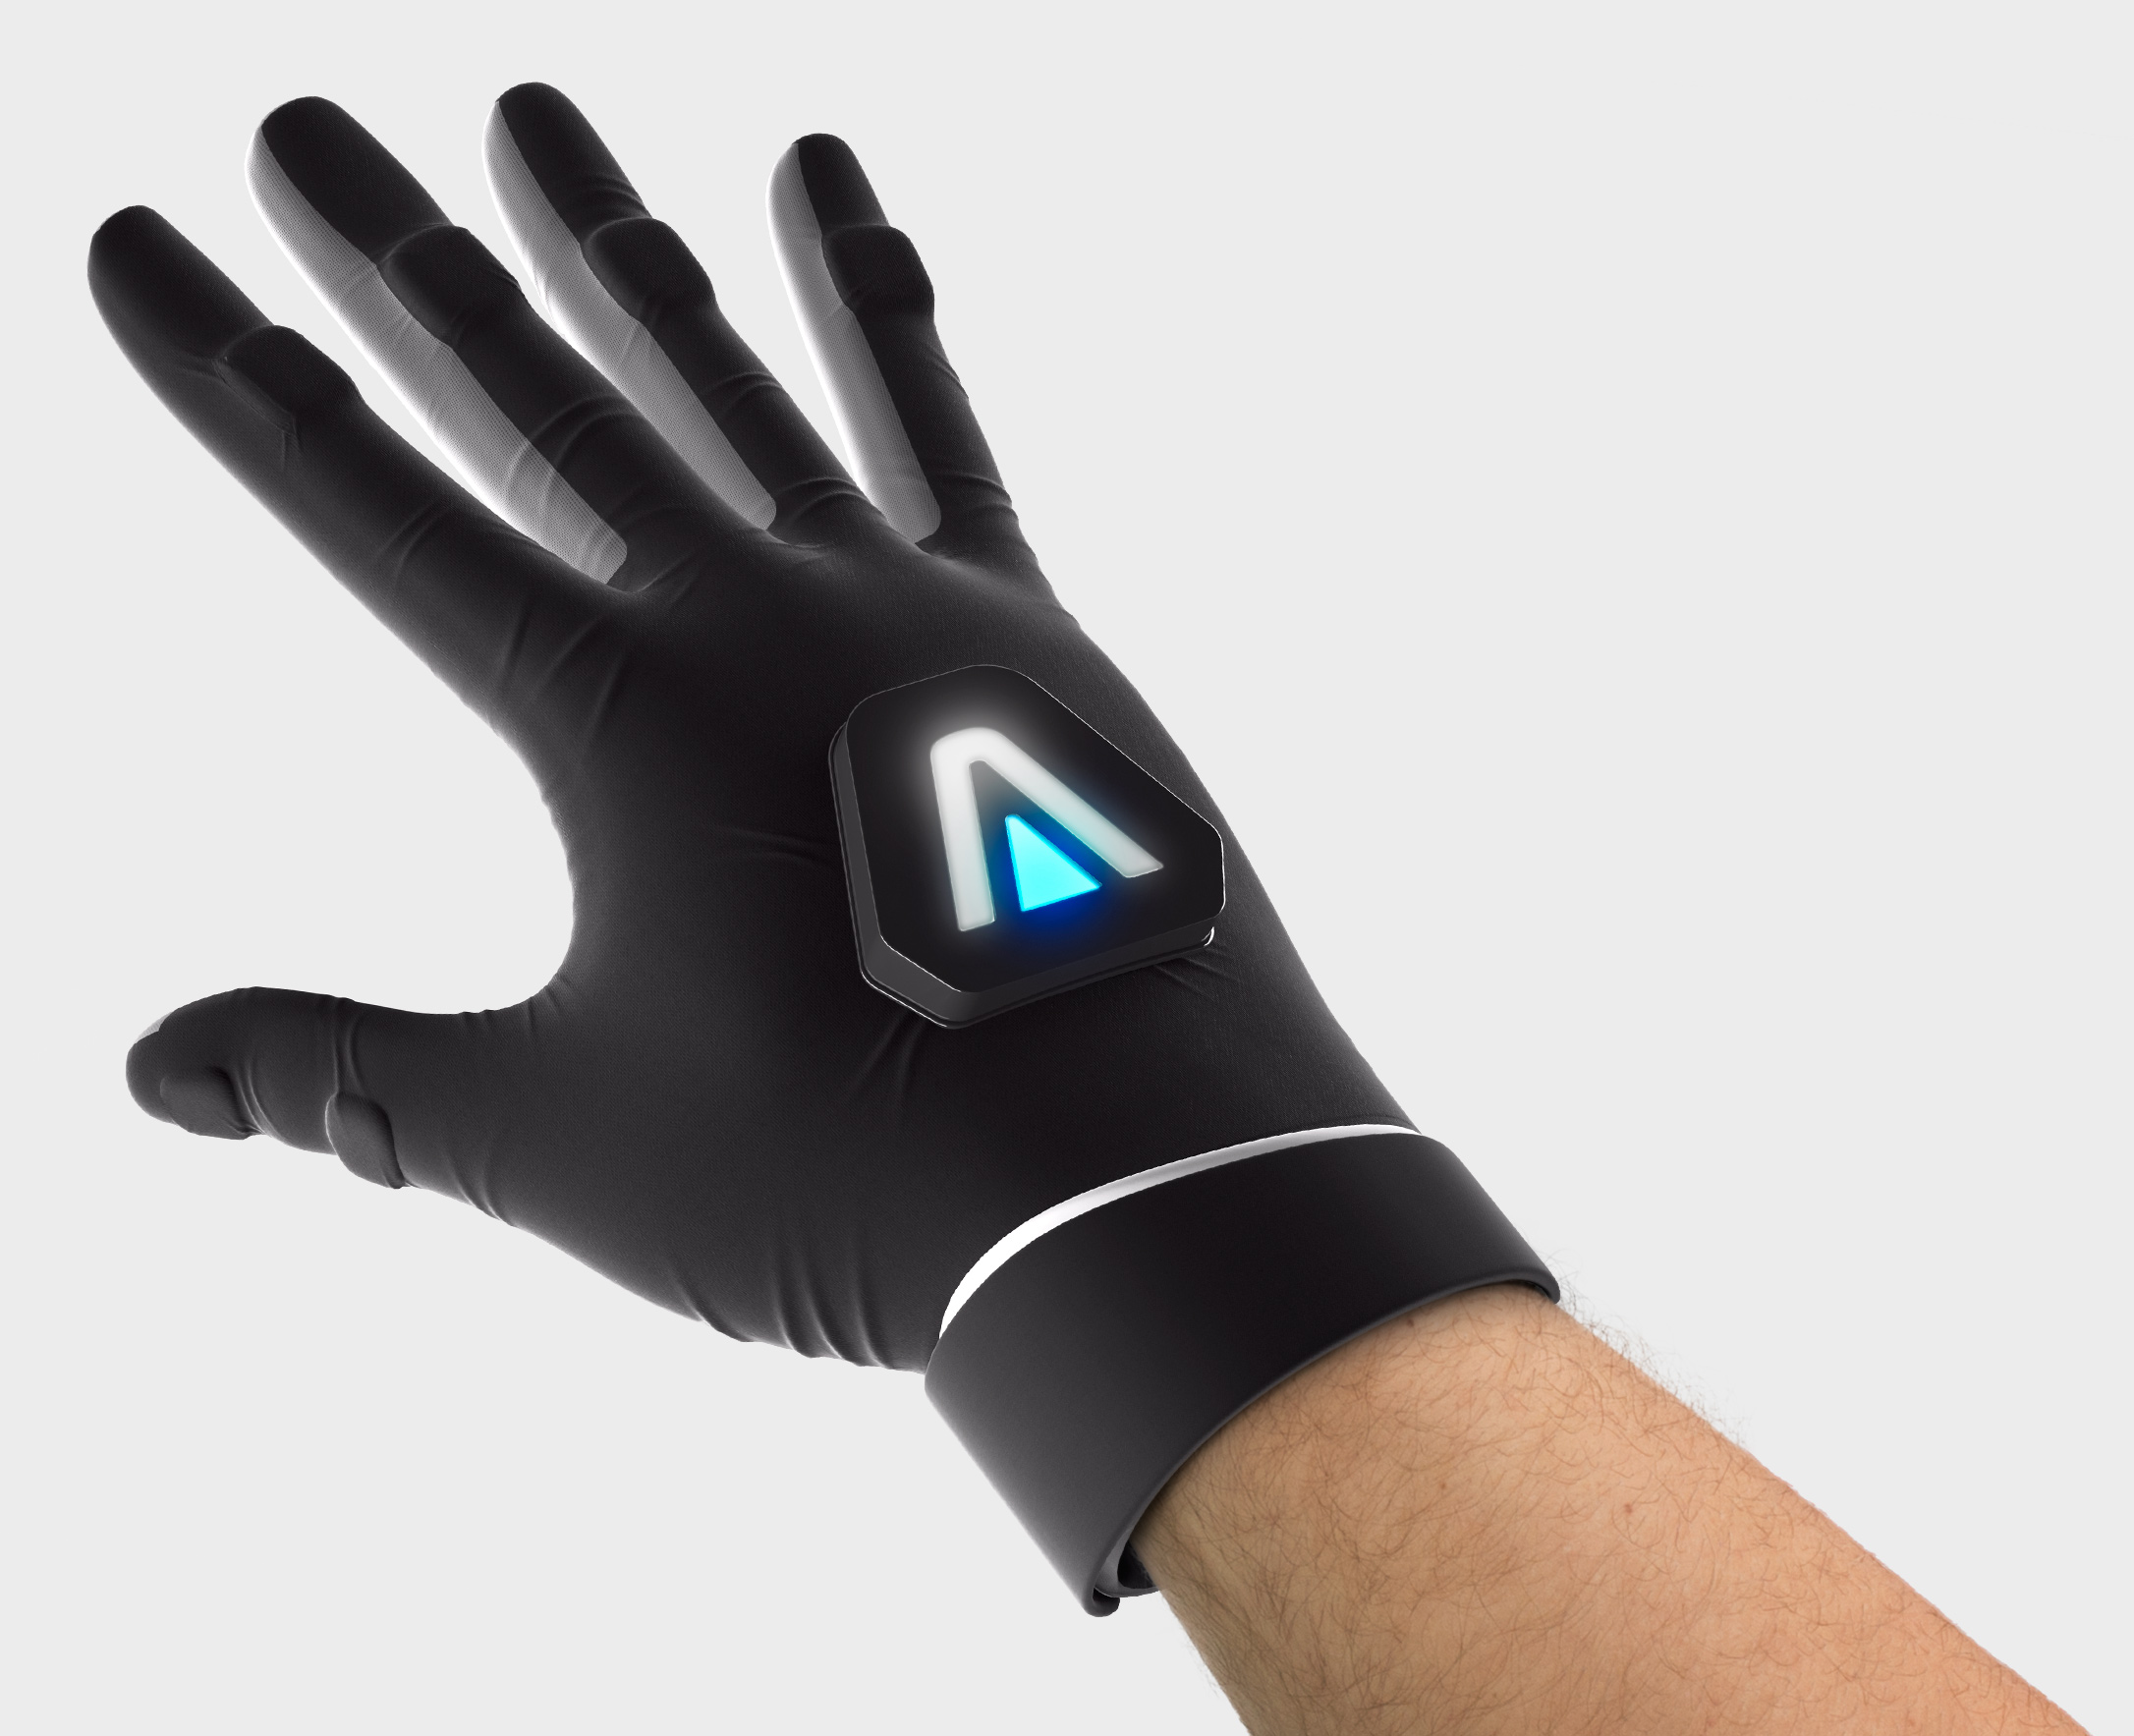
\includegraphics[height=5cm]{imagem/AvatarVR3}\label{fig:avatar}}
  \\
  \subfloat[Cyber Glove III]{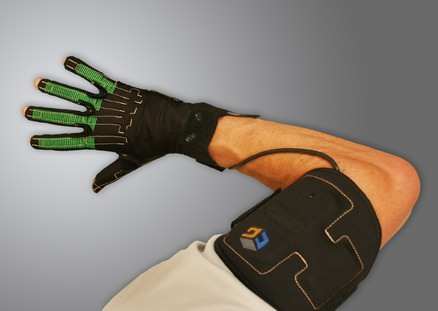
\includegraphics[height=5cm]{imagem/cg3p}\label{fig:cyberglove}}
  \quad
  \subfloat[Manus VR]{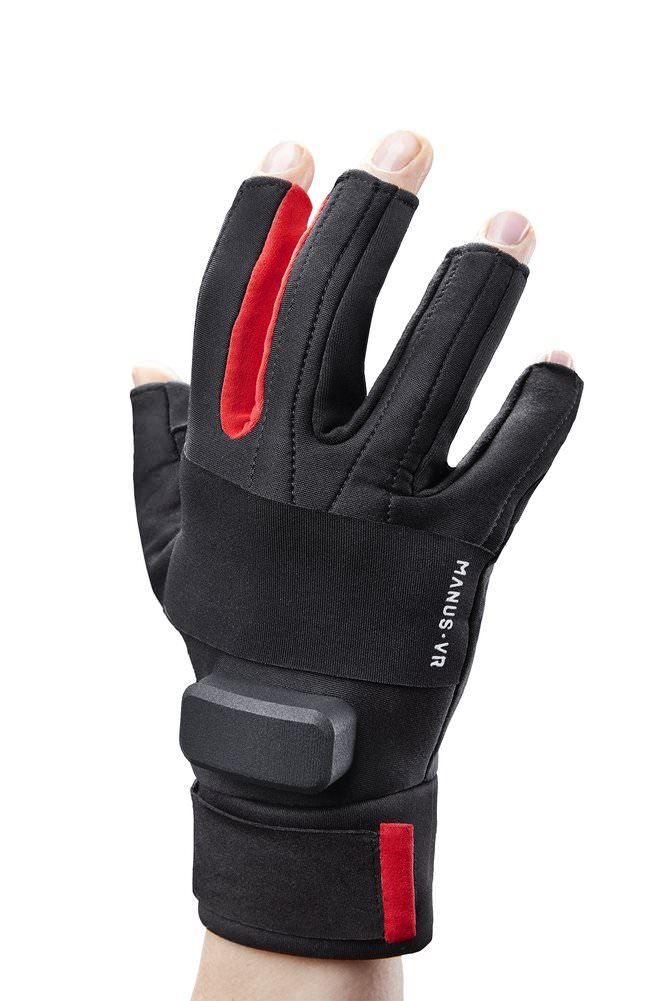
\includegraphics[height=5cm]{imagem/ManusVR}\label{fig:manus}}
  % Caption centralizada
  \captionsetup{justification=centering}
  \captionfont{\small{\textbf{\\Fontes:  \citeonline{5dt},
  \citeonline{avatar}, \citeonline{cyberglove}, \citeonline{manus}}}}
  \label{fig:luvas}
\end{figure}

A \textit{CyberGlove III} (Figura \ref{fig:cyberglove}) produzida pela \textit{CyberGlove Systems} é bastante utilizada em pesquisas acadêmicas, como por exemplo no trabalho realizado por \citeonline{perez2014objective}, que tinha por objetivo analisar a Ergonomia de cirurgiões ao realizar uma cirurgia de laparoscopia\footnote{``A laparoscopia é uma técnica de cirúrgica minimamente invasiva, na qual são utilizadas apenas pequenas incisões entre 0,5 e 1,0 cm para observar o interior da cavidade abdominal e os órgãos aí presentes.'' \cite{laparos}.}, capturando os movimentos do pulso e dos dedos dos cirurgiões. A \textit{5DT Data Glove 5 Ultra} (Figura \ref{fig:5dt}) produzida pela \textit{Fifth Dimensional Technologies} é outra luva eletrônica para utilização em captura de movimentos para animações realistas em tempo-real \cite{5dt}. Seu diferencial é o fato de utilizar sensores de fibra óptica para detectar o flexionamento dos dedos.

Atualmente, novas luvas eletrônicas estão sendo desenvolvidas com o objetivo de serem utilizadas em aplicações de \ac{RV} ou \ac{RA}\footnote{\ac{RV} diz respeito ao ambiente completamente virtual onde o usuário não tem contato com o mundo real. \ac{RA} permite que objetos virtuais sejam adicionados ao ambiente real \cite{azuma1997survey}}
. Dois exemplos notáveis são a \textit{Manus VR} (Figura \ref{fig:manus}) e a \textit{Avatar VR} (Figura \ref{fig:avatar}) que diferem das luvas citadas anteriormente pois, além de sensores de flexão, utilizam também as chamadas Unidades de Medição Inercial (\acf{IMU}). A Tabela \ref{tab:comp} mostra uma comparação entre os modelos de luvas citados nesta seção. Percebe-se que, dentre as luvas analisadas, a \textit{5DT Data Glove Ultra} é a única que utiliza sensores baseados em fibra ótica, com um sensor por dedo. Também nota-se que o preço da \textit{Cyber Glove III} é o mais caro entre eles\footnote{Preço informado pelo fornecedor}, devido à sua grande quantidade de sensores utilizados, sendo 13 vezes mais cara que a 5DT Data Glove Ultra.

\begin{table}[H]
    \centering
    \footnotesize
    \setlength{\abovecaptionskip}{0pt}
    \setlength{\belowcaptionskip}{0pt}
    \caption[Comparação entre modelos de luvas eletrônicas]{Comparação entre modelos de luvas eletrônicas}
    \label{tab:comp}
    \begin{tabularx}{\textwidth}{p{3.7cm}XXrr}
      \hline\hline
      \multicolumn{1}{c}{Luvas} & \multicolumn{1}{c}{Interface} & \multicolumn{1}{c}{Tipo de Sensor} & \multicolumn{1}{c}{Nº de Sensores} & \multicolumn{1}{c}{Preço por Mão}\\
      \hline
      5DT Data Glove 5 Ultra    & USB                           & Fibra óptica                       & 5                                  & US\$995\\
      Avatar VR                 & WiFi                          & \ac{IMU}                           & 6                                  & \euro{1100}\\
      CyberGlove III            & WiFi e USB                    & Flexão                             & 18 ou 22                           & US\$12995\\
      Manus VR                  & WiFi                          & \ac{IMU}/Flexão                    & 1 \ac{IMU} + 5 Flexão              & US\$250\\
      \hline \hline
    \end{tabularx}
    \\\vspace{1.3mm}
    \captionfont{\small{\textbf{Fontes: \citeonline{5dt}, \citeonline{avatar}, \citeonline{cyberglove}, \citeonline{manus}, \citeonline{manus_specs}}}}
  \end{table}

Uma das grandes dificuldades na evolução de luvas eletrônicas está na grande quantidade de movimentos que podem ser exercidos pela mão humana, tornando complexa a sua captação e reprodução fiel por computadores ou braços robóticos. Outro fator limitante é o alto custo dos dispositivos utilizados para a fabricação de luvas eletrônicas, sendo necessários sensores com alta precisão e repetibilidade, além de serem compactos e leves a fim de não limitar os movimentos do usuário final.

\section{Sensores}
\label{sec:sens}
Um sensor é ``um dispositivo que detecta mudanças em um estímulo físico e as transformam em um sinal que pode ser medido ou gravado.''\cite{sensor}\footnote{``[\ldots] a device that detects a change in a physical stimulus and turns it into a signal which can be measured or recorded [\ldots]''}. Os sensores utilizados em luvas eletrônicas podem ser:
\begin{enumerate}
\item[a)] flexão -- mede deformações (dobras) em sua superfície. São utilizados para detectar o movimento de flexão e extensão dos dedos;
\item[b)] acelerômetro -- mede a aceleração física exercida sobre ele. São utilizados para detectar a rotação da mão no espaço.
\end{enumerate}

\subsection{Sensor de flexão baseado em tinta resistiva}
\label{subsec:flextin}

Estes são sensores passivos que possuem uma camada de tinta resistiva sobre uma tira de plástico flexível (Figura \ref{fig:flextinta}). Quando o sensor está plano (Figura \ref{fig:plano}), ele possui um valor de resistência elétrica, e, quando flexionado (Figura \ref{fig:curvo}), as partículas condutivas da tinta se afastam, dificultando a passagem de elétrons, aumentando sua resistência.

\begin{figure}[H]
  \centering
  % Alterar espaçamentos antes e depois do caption
  \setlength{\abovecaptionskip}{0pt}
  \setlength{\belowcaptionskip}{0pt}
  % Caption
  \caption[Funcionamento do sensor de flexão]{Funcionamento do sensor de flexão}
    \subfloat[Partículas condutivas próximas]{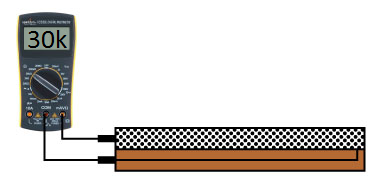
\includegraphics[width=.5\textwidth]{imagem/sensor_reto}\label{fig:plano}}\\
    \subfloat[Partículas condutivas afastadas]{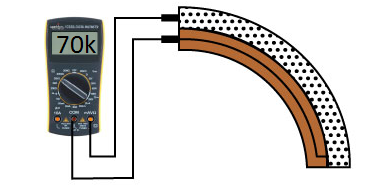
\includegraphics[width=.5\textwidth]{imagem/sensor_curvo}\label{fig:curvo}}
  % Caption centralizada
  \captionsetup{justification=centering}
  \captionfont{\small{\textbf{\\Fontes: \citeonline{sparkflex}}}} 
  \label{fig:sensorflex}
\end{figure}

\begin{figure}[H]
  \setlength{\abovecaptionskip}{0pt}
  \setlength{\belowcaptionskip}{0pt}
  \caption[Sensor de flexão baseado em tinta resistiva]{Sensor de flexão baseado em tinta resistiva}
  \centering
  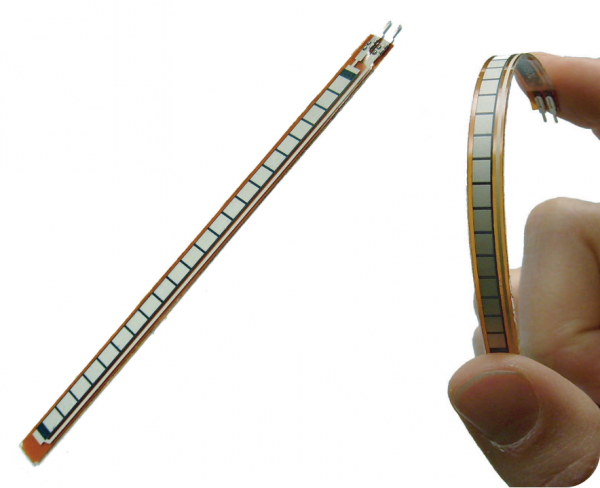
\includegraphics[width=.4\textwidth]{imagem/flexsensordirection}
  \captionsetup{justification=centering}
  \captionfont{\small{\textbf{\\Fonte: \citeonline{symbol2012flex}}}}
  \label{fig:flextinta}
\end{figure}

\subsection{Sensor de flexão baseado em fibra ótica}
\label{subsec:flexotic}
Os sensores baseados em fibra ótica (Figura \ref{fig:flexotico}) possuem um emissor de luz em uma extremidade e um receptor em outra. Quando o sensor é flexionado, a intensidade de luz que chega no receptor é diminuída devido às reflexões que ocorrem no interior da fibra ótica. Essa diferença de intensidade é medida e indica quanto o sensor foi flexionado.

\begin{figure}[H]
  \setlength{\abovecaptionskip}{0pt}
  \setlength{\belowcaptionskip}{0pt}
  \caption[Sensor de flexão baseado em fibra ótica]{Sensor de flexão baseado em fibra ótica}
  \centering
  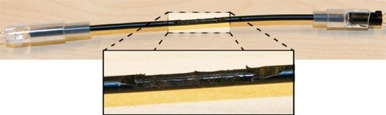
\includegraphics[width=.5\textwidth]{imagem/twend-optical}
  \captionsetup{justification=centering}
  \captionfont{\small{\textbf{\\Fonte: \citeonline{herkenrath2008twend}}}}
  \label{fig:flexotico}
\end{figure}

\subsection{\acf{IMU}}
\label{subsec:imu}
\ac{IMU}s são dispositivos que utilizam uma combinação de acelerômetros, giroscópios e, em alguns casos, magnetômetros para medir as diferentes forças que atuam sobre esse sensor, como aceleração, rotação ou campo magnético. Um \ac{IMU} consegue detectar translação e rotação em cada um dos eixos $X$, $Y$ e $Z$, totalizando 6 \ac{DOF} (Figura \ref{fig:imu}). 

\begin{figure}[H]
  \setlength{\abovecaptionskip}{0pt}
  \setlength{\belowcaptionskip}{0pt}
  \caption[Eixos de detecção de um \ac{IMU}]{Eixos de detecção de um \ac{IMU}}
  \centering
  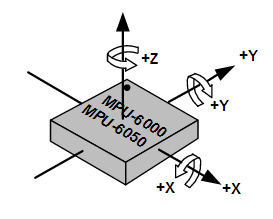
\includegraphics[width=.4\textwidth]{imagem/IMU_eixos}
  \captionsetup{justification=centering}
  \captionfont{\small{\textbf{\\Fonte: \citeonline{IMU}}}}
  \label{fig:imu}
\end{figure}

\subsubsection{Acelerômetro}
\label{subsubsec:accel}
Acelerômetros são dispositivos que medem a intensidade da força de aceleração exercida sobre ele. Geralmente possuem uma massa móvel suspensa por molas e, ao movimentar o dispositivo, a massa se desloca, deformando as molas e gerando um sinal elétrico que é medido para informar em que direção e com qual intensidade ocorreu a aceleração. Por exemplo, um acelerômetro em descanso na superfície da Terra medirá uma aceleração de aproximadamente \SI{9.81}{m/s^{2}} sobre o eixo $Z$, ou seja, a aceleração da gravidade. Acelerômetros detectam movimentos de translação nos eixos $X$, $Y$ e $Z$ do espaço, por isso possui 3 \ac{DOF} (Figura \ref{fig:accel}).

\begin{figure}[H]
  \setlength{\abovecaptionskip}{0pt}
  \setlength{\belowcaptionskip}{0pt}
  \caption[Estrutura do acelerômetro]{Estrutura do acelerômetro}
  \centering
  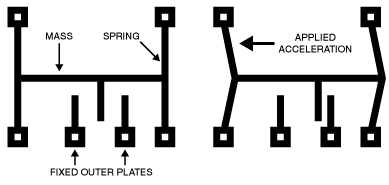
\includegraphics[width=.4\textwidth]{imagem/accel}
  \captionsetup{justification=centering}
  \captionfont{\small{\textbf{\\Fonte: \citeonline{accel}}}}
  \label{fig:accel}
\end{figure}

\subsubsection{Giroscópio}
\label{subsubsec:gyro}
Giroscópios detectam a rotação em torno de cada um dos eixos $X$, $Y$ e $Z$, ou seja, a velocidade angular ou a taxa de variação do ângulo de rotação em graus por segundo (\SI[per-mode=symbol]{}{\degree\per\second}). Existem três tipos básicos de giroscópios: Rotatórios, Ópticos e Vibratórios \cite{fraden2004handbook}, sendo este último o mais comum em circuitos integrados, pois tem menor tamanho em relação aos outros tipos. Eles possuem uma massa conectada por molas a uma estrutura, que por sua vez está conectada a uma segunda estrutura fixa no circuito (Figura \ref{fig:gyro}) . A massa central oscila verticalmente e, quando o giroscópio é submetido a uma rotação, a estrutura se move na horizontal, devido à força inercial de Coriolis\footnote{``A força de Coriolis é uma força que surge num sistema referencial em rotação que tende a alterar a trajetória dos corpos em movimento.'' \cite{coriolis}}. Como o giroscópio não possui uma referência fixa para suas medições, ele é suscetível a erros cumulativos ao longo do tempo, conforme sua utilização ou temperatura.

\begin{figure}[H]
  \setlength{\abovecaptionskip}{0pt}
  \setlength{\belowcaptionskip}{0pt}
  \caption[Estrutura do giroscópio]{Estrutura do giroscópio}
  \centering
  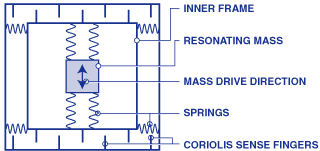
\includegraphics[width=.4\textwidth]{imagem/gyro_vsg1}
  \captionsetup{justification=centering}
  \captionfont{\small{\textbf{\\Fonte: \citeonline{gyroscope}}}}
  \label{fig:gyro}
\end{figure}

\subsubsection{Magnetômetro}
\label{subsubsec:mag}
Magnetômetros são sensores que detectam o efeito de Hall\footnote{ o efeito de Hall se refere ao desvio da trajetória normal das cargas fluindo em um semicondutor, quando este é submetido à ação de um campo magnético. Este desvio causa uma diferença de potencial que pode ser medida perpendicularmente ao sentido do movimento da corrente.\cite{hall}} (Figura \ref{fig:mag}). Quando a \ac{IMU} utiliza um magnetômetro, é possível detectar a intensidade do campo magnético em torno do dispositivo.

\begin{figure}[H]
  \setlength{\abovecaptionskip}{0pt}
  \setlength{\belowcaptionskip}{0pt}
  \caption[Demonstração do Efeito de Hall]{Demonstração do Efeito de Hall}
  \centering
  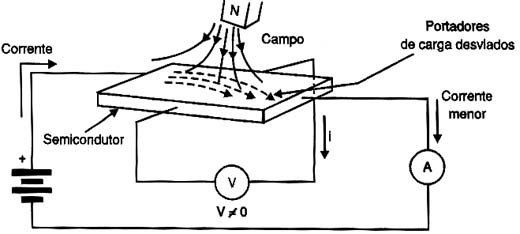
\includegraphics[width=.4\textwidth]{imagem/hall}
  \captionsetup{justification=centering}
  \captionfont{\small{\textbf{\\Fonte: \citeonline{hall}}}}
  \label{fig:mag}
\end{figure}

Nas \ac{IMU}s, os dados do acelerômetro, giroscópio e magnetômetro geralmente são usados em conjunto para fornecer leituras de orientação precisas, já que os dados do acelerômetro são muito ruidosos, o giroscópio é suscetível a erros cumulativos e o magnetômetro sofre interferência de campos magnéticos externos. As leituras suaves do giroscópio são combinadas com as do acelerômetro para reduzir ruídos, e as leituras do magnetômetro são usadas para detectar o campo magnético da Terra, sendo este usado como referência para calcular a orientação e também para corrigir os erros provenientes do giroscópio.%

\section{Trabalhos Relacionados}%
\label{sec:trabrel}%
Em \citeonline{fang2015robotic}, foi proposta uma luva eletrônica  composta de 18 \ac{IMMU} para controle remoto de um braço robótico. Dos \ac{IMMU} utilizados, 15 foram acoplados em cada um dos segmentos dos dedos, um na palma da mão, um no antebraço e um no braço (Figura \ref{fig:2015luva}). O robô controlado pela luva possui braço com 7 \ac{DOF}, mão com 4 \ac{DOF} e os dados das \ac{IMMU} foram mapeados em cada segmento do robô, de modo que as informações geradas pelas \ac{IMMU} são convertidas em instruções para controle do braço e da mão robótica (Figura \ref{fig:2015robo}). O primeiro teste executado foi para verificar o funcionamento correto da luva e das informações geradas, resultando em um erro médio quadrado das orientações no eixos $X$, $Y$ e $Z$ de menos de \ang{0.5}. Os próximos testes consistiram em controlar a mão e o braço robótico remotamente (Figura \ref{fig:2015controle}), mostrando que os movimentos realizados foram suaves e imitavam o movimento do braço do operador. Este trabalho mostra que, dado um sistema de captura adequado, é possível mapear os movimentos realizados por um humano em instruções de movimento de robôs através da utilização de sensores. Esse tipo de controle permite que braços robóticos sejam operados intuitivamente e com movimentos naturais. Entretanto, essa solução prioriza a captura do braço e antebraço e não os movimentos específicos da mão, que são necessários para o problema proposto nesse trabalho.

\begin{figure}[h]
  \centering
  \setlength{\abovecaptionskip}{0pt}
  \setlength{\belowcaptionskip}{0pt}
  \caption[Luva e Robô desenvolvidos por \citeonline{fang2015robotic}]{Luva e Robô desenvolvidos por \citeonline{fang2015robotic}}
    \subfloat[Luva]{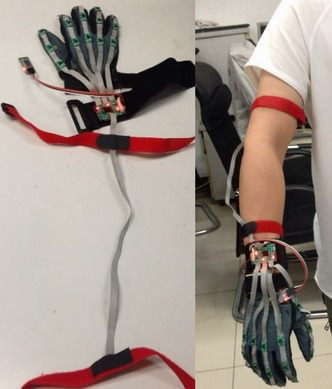
\includegraphics[height=5cm]{imagem/2015luva}\label{fig:2015luva}}
    \quad
    \subfloat[Robô]{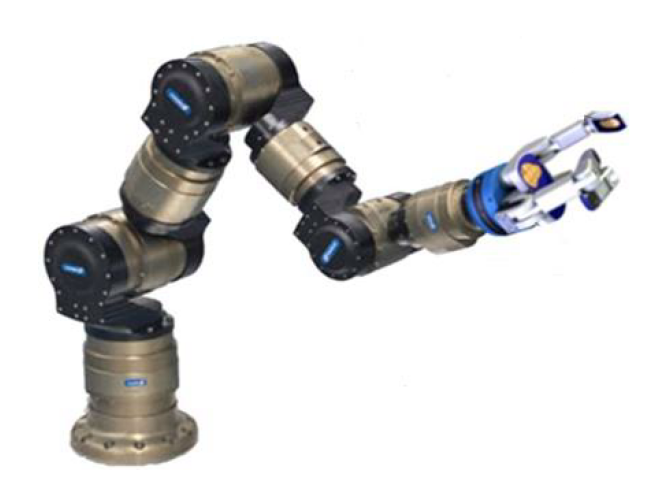
\includegraphics[height=5cm]{imagem/2015robo}\label{fig:2015robo}}\\
    \subfloat[Controle do Robô com a Luva]{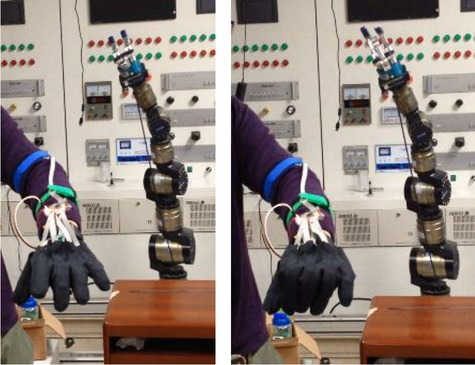
\includegraphics[width=.5\textwidth]{imagem/2015controle}\label{fig:2015controle}}
  \captionsetup{justification=centering}
  \captionfont{\small{\textbf{\\Fontes: \citeonline{fang2015robotic}}}}
  \label{fig:fang}
\end{figure}

Em \citeonline{fahn2005development}, foi desenvolvida uma luva eletrônica utilizando bobinas de indução magnética como sensores de movimento dos dedos. Utilizou-se três bobinas por dedo, duas geradoras de campo magnético e uma para medir a variação desse campo. Elas foram posicionadas sob os dedos, na região palmar (Figura \ref{fig:magneto}), para que o sinal da força eletromotriz, gerada pela variação do campo magnético, fosse grande o suficiente para se realizar as medições com precisão. Os autores ainda propuseram um método de calibração da luva que consistia em dois movimentos simples, sendo o primeiro com a mão aberta com os dedos esticados, e o segundo, com a mão fechada segurando um cilindro de modo que os ângulos formados com a primeira falange fossem de aproximadamente \ang{90}. Para prevenir interferências entre as bobinas, foi definido um tempo de ativação para cada bobina geradora, no qual o resultado das bobinas receptoras era detectado e enviado para um conversor \ac{A/D} que enviava os sinais para um microcontrolador para o processamento. Este método para captura do movimento dos dedos, embora preciso, é complexo computacionalmente devido aos cálculos envolvidos para obter os ângulos de dobra dos dedos. Além disso, este método é sensível à interferência de campos magnéticos exteriores.

\begin{figure}[H]
  \setlength{\abovecaptionskip}{0pt}
  \setlength{\belowcaptionskip}{0pt}
  \caption[Posicionamento das bobinas sensoras e geradoras]{Posicionamento das bobinas sensoras e geradoras}
  \centering
  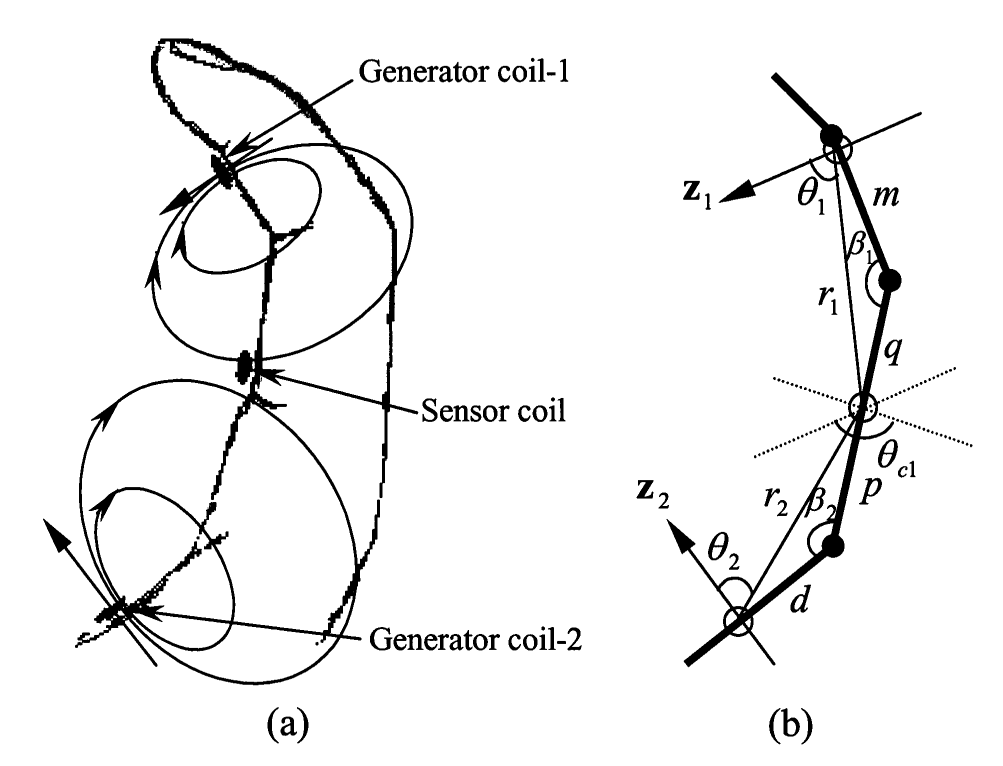
\includegraphics[width=.5\textwidth]{imagem/2005magneto}
  \captionsetup{justification=centering}
  \captionfont{\small{\textbf{\\Fonte: \citeonline{fahn2005development}}}}
  \label{fig:magneto}
\end{figure}


No trabalho de \citeonline{kim20093}, foi criada uma luva para reconhecimento de gestos utilizando três acelerômetros com 3 \ac{DOF} denominada \textit{KHU-1}. Um dos acelerômetros foi posicionado na região dorsal da mão para detectar sua orientação espacial, outro posicionado no polegar e o último posicionado no dedo médio, controlando os movimentos dos dedos indicador, médio, anelar e mínimo (Figura \ref{fig:2009accel}). A comunicação com o computador foi feita através de \textit{Bluetooth} para controlar um modelo \ac{3D} da mão. Os testes para reconhecimento de gestos consistiram na realização dos movimentos de ``pedra'', ``papel'' e ``tesoura'', com a mão na vertical, horizontal com palma para baixo e horizontal com palma para cima. A luva obteve taxa de acerto total no reconhecimento desses gestos, porém os autores não detalharam os procedimentos utilizados para validação dos testes. Uma das desvantagens desse projeto é que não há independência entre os dedos já que todos são controlados pelo dedo médio.

\begin{figure}[H]
  \setlength{\abovecaptionskip}{0pt}
  \setlength{\belowcaptionskip}{0pt}
  \caption[A luva \textit{KHU-1}]{A luva \textit{KHU-1}}
  \centering
  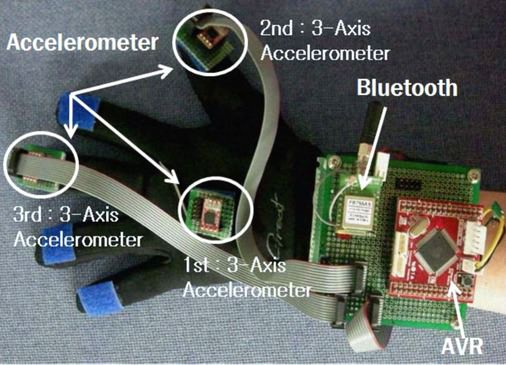
\includegraphics[width=.5\textwidth]{imagem/2009accel}
  \captionsetup{justification=centering}
  \captionfont{\small{\textbf{\\Fonte: \citeonline{kim20093}}}}
  \label{fig:2009accel}
\end{figure}

\citeonline{li2009smartglove} apresenta o desenvolvimento de uma luva eletrônica chamada \textit{SmartGlove} e de um \textit{encoder} linear ótico para detectar o ângulo de dobra de múltiplas articulações dos dedos (Figura \ref{fig:2009smartglove}). Os \textit{encoders} foram construídos com base em sensores de \textit{mouse} ótico e foram conectados a uma fita fixa na região dorsal da mão, que se deslocava sob os dedos quando eles se articulavam, possibilitando que um microcontrolador calculasse o ângulo dessa articulação baseado no movimento da fita detectado pelo sensor. A luva produzida possuía baixo custo devido aos materiais utilizados, fornecendo sensores com boa linearidade (\SI{99.4}{\percent} quando o dedo era dobrado) e precisão (menos de \ang{1} comparado ao acelerômetro), sendo leve e não intrusiva ao usuário. Os testes de verificação de linearidade e precisão dos sensores realizados pelo autor podem ser adotados para as luvas que detectam o ângulo de dobra das articulações, como é o caso da luva proposta neste trabalho.

\begin{figure}[H]
  \setlength{\abovecaptionskip}{0pt}
  \setlength{\belowcaptionskip}{0pt}
  \caption[Princípio de funcionamento da \textit{SmartGlove}]{Princípio de funcionamento da \textit{SmartGlove}}
  \centering
  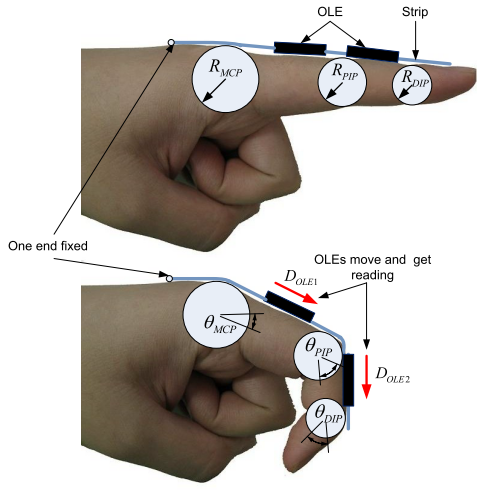
\includegraphics[width=.5\textwidth]{imagem/2009smartglove}
  \captionsetup{justification=centering}
  \captionfont{\small{\textbf{\\Fonte: \citeonline{li2009smartglove}}}}
  \label{fig:2009smartglove}
\end{figure}

O projeto de \citeonline{leap} é um dispositivo que utiliza giroscópios em conjunto com o \textit{Leap Motion}, que é um sensor que detecta movimentos no espaço, para criar um controle de \ac{RV} que é simples e não intrusivo. O sensor \textit{Leap Motion} fica afixado em um \textit{display} de \acl{RV} capturando os movimentos das mãos do usuário e, o giroscópio fica preso na palma da mão do usuário junto com dois botões para interação com o ambiente virtual (Figura \ref{fig:leap}). O projeto ainda está em desenvolvimento, mas se mostra uma técnica interessante para captura do movimentos e da orientação da mão em ambientes \ac{3D}.

\begin{figure}[H]
  \setlength{\abovecaptionskip}{0pt}
  \setlength{\belowcaptionskip}{0pt}
  \caption[Controle de \ac{RV}]{Controle de \ac{RV} de \citeonline{leap}}
  \centering
  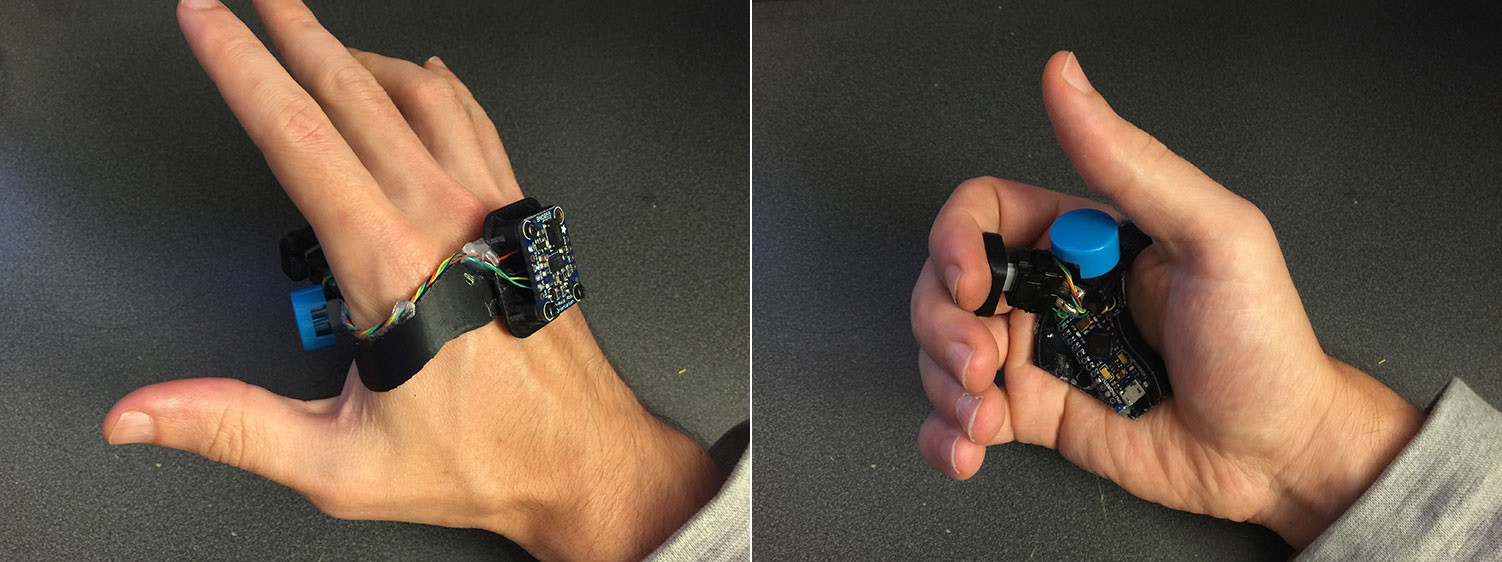
\includegraphics[height=4.5cm]{imagem/leap}
  \captionsetup{justification=centering}
  \captionfont{\small{\textbf{\\Fonte: \citeonline{leap}}}}
  \label{fig:leap}
\end{figure}

O presente trabalho baseia-se na continuidade do trabalho de \citeonline{roversi}, que consistiu no desenvolvimento de um protótipo de luva eletrônica de baixo custo, utilizando sensores de flexão baseados em tinta resistiva para detecção do movimento dos dedos, e uma \ac{IMU} para detecção da orientação da mão, acoplados à plataforma Arduino (Figura \ref{fig:luvaroversi}). No trabalho do autor, foram utilizados dois sensores de flexão em cada dedo a fim de detectar a articulação da primeira falange independentemente das articulações da segunda e terceira falanges. Para os testes, foi modelada uma mão \ac{3D} no ambiente de desenvolvimento de jogos \citeonline{unity}, e os movimentos realizados pelo usuário deveriam ser reproduzidos na mão virtual. Um dos problemas dessa luva foi o fato de ela não reproduzir movimentos de adução e abdução dos dedos ou de desvio radial e ulnar do pulso.

\begin{figure}[H]
  \setlength{\abovecaptionskip}{0pt}
  \setlength{\belowcaptionskip}{0pt}
  \caption[A luva de \citeonline{roversi}]{A luva de \citeonline{roversi}}
  \centering
  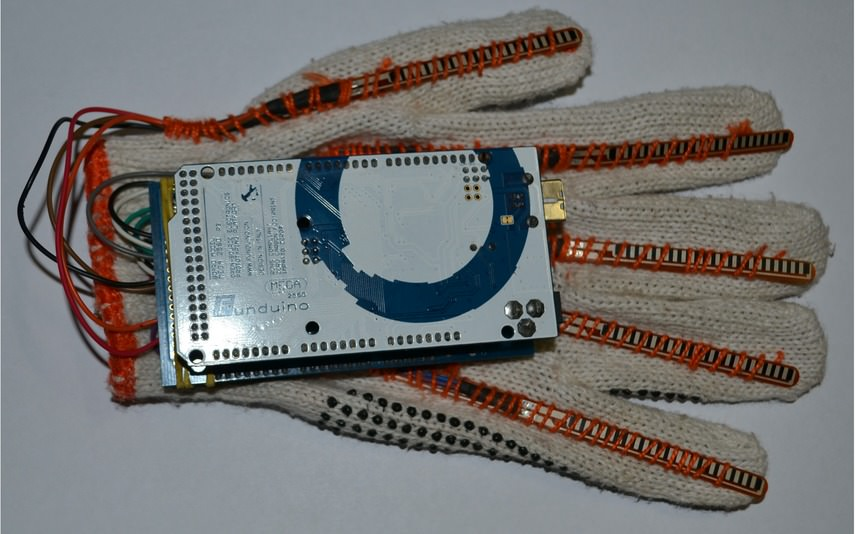
\includegraphics[width=.5\textwidth]{imagem/2016roversi}
  \captionsetup{justification=centering}
  \captionfont{\small{\textbf{\\Fonte: \citeonline{roversi}}}}
  \label{fig:luvaroversi}
\end{figure}

% Nome do capítulo
\chapter{Metodologia}
% Label para referenciar
\label{ch:meto}

% Diminuir espaçamento entre título e texto
\vspace{-1.9cm}
Os componentes utilizados para a execução desse projeto são um \textit{Arduino Mega 2560}, 14 sensores de flexão, e duas \ac{IMU}s \textit{MPU-9250}. O motivo da escolha destes componentes será explicado na Seção \ref{sec:hardware}.

Para a execução desse projeto foi construído um novo protótipo baseado na luva de \citeonline{roversi} (Figura \ref{fig:luvaorig}), que possui as seguintes limitações:

\begin{compactitem}
  \item[a)] não detecta movimentos de adução e abdução dos dedos;
  \item[b)] não detecta movimentos de desvio radial e ulnar do pulso;
  \item[c)] ruídos provenientes da \ac{IMU} utilizada;
  \item[d)] sensores de flexão não estão propriamente posicionados.
\end{compactitem}

Para solucionar o problema da detecção dos movimentos de adução e abdução, foram utilizados mais quatro sensores de flexão posicionados entre cada par dedos. Os dados gerados por esses sensores foram transformados no ângulo de abertura formado entre os dedos e fornecidos ao \textit{script} da \textit{Unity} para animação do modelo \ac{3D} da mão. Para captura dos dados de orientação da mão foram utilizadas duas \ac{IMU}s \textit{MPU-9250}, uma nas costas da mão e outra acima do pulso, no antebraço, de modo que as diferenças entre os ângulos de orientação das duas \ac{IMU}s fornecessem o ângulo de dobra entre o pulso e o antebraço, o que corresponderia aos movimentos de desvio radial e ulnar do pulso. A Figura \ref{fig:novaluva} mostra o diagrama de posicionamento dos componentes na luva para a solução dos problemas propostos.

O sinal de orientação que é enviado pelo \textit{Arduino} é bastante ruidoso, causando instabilidade no modelo \ac{3D} e fazendo-o tremer. Tal ruído é proveniente do acelerômetro, pois este é impreciso para fornecer dados do ângulo de orientação do sensor, portanto leituras somente do acelerômetro não podem ser utilizadas. Por outro lado, o giroscópio fornece dados estáveis de ângulo, mas pequenos erros de leitura acumulam-se com o tempo, fornecendo dados incorretos (efeito conhecido como \textit{drift}). A solução é utilizar as leituras do acelerômetro e do giroscópio em conjunto para obter valores mais próximos dos reais. A \ac{IMU} \textit{MPU-9250} possui um processador interno chamado de \ac{DMP} que realiza a fusão e filtragem dos dados do acelerômetro, giroscópio e magnetômetro e fornece a orientação da \ac{IMU} sem a necessidade de utilizar o processador do \textit{Arduino} para isso.

\begin{figure}[H]
  \setlength{\abovecaptionskip}{0pt}
  \setlength{\belowcaptionskip}{0pt}
  \caption[Diagrama da Luva]{Diagrama da Luva}
  \centering
  \subfloat[Protótipo original]{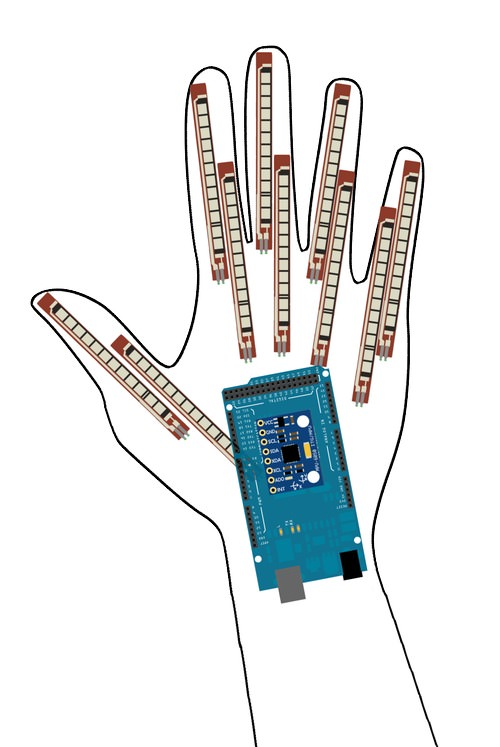
\includegraphics[width=.45\textwidth]{imagem/Luva_Atual}\label{fig:luvaorig}}
  \subfloat[Novo protótipo]{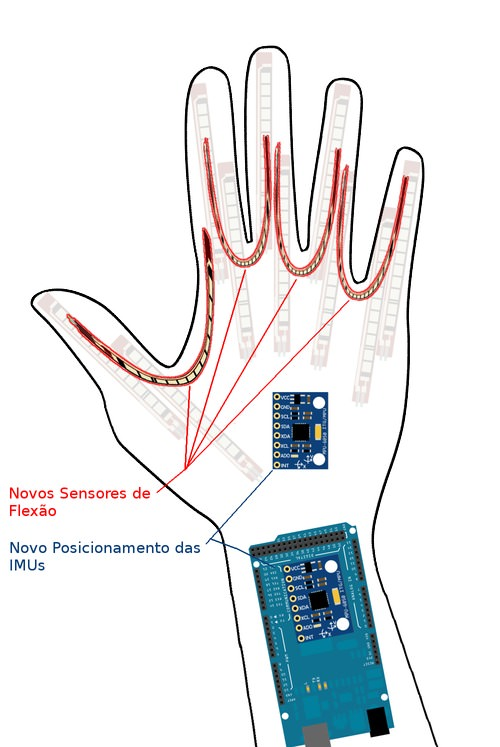
\includegraphics[width=.45\textwidth]{imagem/Nova_Luva}\label{fig:novaluva}}
  \captionsetup{justification=centering}
  \captionfont{\small{\textbf{\\Fonte: Elaborado pelo Autor}}}
  \label{fig:diagluva}
\end{figure}

A verificação do funcionamento correto da luva e análise da redução de ruídos foi feita observando os valores da média, \ac{DP}, amplitude e \ac{DMA} dos valores brutos recebidos dos sensores.

\section{Diagrama de Arquitetura}
\label{sec:arquitetura}
O diagrama da Figura \ref{fig:arq} representa a arquitetura do projeto, mostrando as conexões entre cada componente. O \textit{Arduino} lê os dados de dobra dos sensores de flexão e os dados de orientação das duas \ac{IMU}s e os envia através de um cabo \ac{USB} para o computador.

\begin{figure}[H]
  \setlength{\abovecaptionskip}{0pt}
  \setlength{\belowcaptionskip}{0pt}
  \caption[Diagrama de arquitetura]{Diagrama de arquitetura}
  \centering
  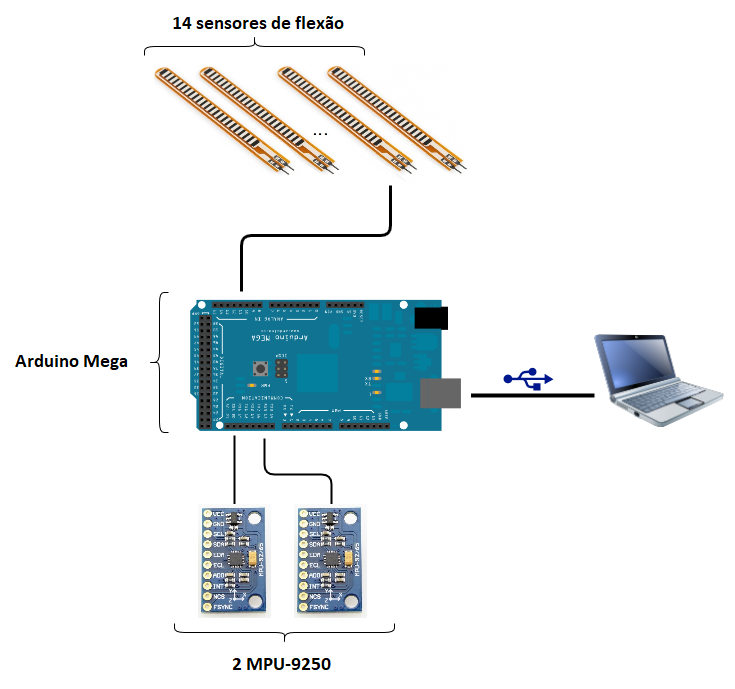
\includegraphics[width=.7\textwidth]{imagem/arquitetura}
  \captionsetup{justification=centering}
  \captionfont{\small{\textbf{\\Fonte: Elaborado pelo Autor}}}
  \label{fig:arq}
\end{figure}

\section{Diagrama de Caso de Uso}
\label{sec:caso_de_uso}
A Figura \ref{fig:uml} apresenta o diagrama de caso de uso do projeto, representando o fluxo de troca de dados entre usuário, \textit{Arduino} e \textit{Unity}.

Primeiro o usuário movimenta a luva, gerando as leituras de ângulos de dobra dos dedos e ângulo de orientação da mão e do braço. Em seguida o \textit{Arduino} recebe esses dados e os prepara para envio pela porta serial do computador para a aplicação \textit{Unity}, que requisita esses dados a cada atualização de \textit{frame}.

\begin{figure}[H]
  \setlength{\abovecaptionskip}{0pt}
  \setlength{\belowcaptionskip}{0pt}
  \caption[Diagrama de caso de uso]{Diagrama de caso de uso}
  \centering
  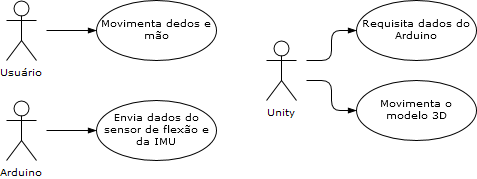
\includegraphics[width=.7\textwidth]{imagem/Caso_de_Uso}
  \captionsetup{justification=centering}
  \captionfont{\small{\textbf{\\Fonte: Elaborado pelo Autor}}}
  \label{fig:uml}
\end{figure}

\section{Diagrama de Sequência}
\label{sec:sequencia}
O diagrama de sequência mostrado na Figura \ref{fig:seq} exibe a sequência de troca de dados entre sensores \textit{Arduino} e \textit{Unity}, desde a captação dos dados até a exibição do resultado na tela. Também é possível observar que os dados mais recentes só são enviados à \textit{Unity} quando ocorre a atualização do \textit{frame}. Isso foi feito para evitar que os valores dos sensores fiquem presos no \textit{buffer} de entrada da porta serial, o que pode resultar em uma resposta lenta do modelo \ac{3D}.

A movimentação da mão do usuário gera as leituras de dobra dos dedos e posição da mão em relação ao braço. Os valores de dobra são lidos pelo \textit{Arduino} através da função \lstinline!Analog.read()! e os valores dos ângulos de orientação da mão são recebidos pelo \textit{Arduino} através da função \lstinline!mpu.dmpGetQuaternion()! do \textit{MPU-9250}. Durante cada atualização de \textit{frame} da \textit{Unity}, é enviado um caractere pela porta serial que serve para requisição dos dados atuais dos sensores. O \textit{Arduino} então lê esse caractere e envia os dados pela porta serial para a \textit{Unity}, que os usa para manipular os objetos na tela através da função \lstinline!transform.localEulerAngles()!.

\begin{figure}[H]
  \setlength{\abovecaptionskip}{0pt}
  \setlength{\belowcaptionskip}{0pt}
  \caption[Diagrama de sequência]{Diagrama de sequência}
  \centering
  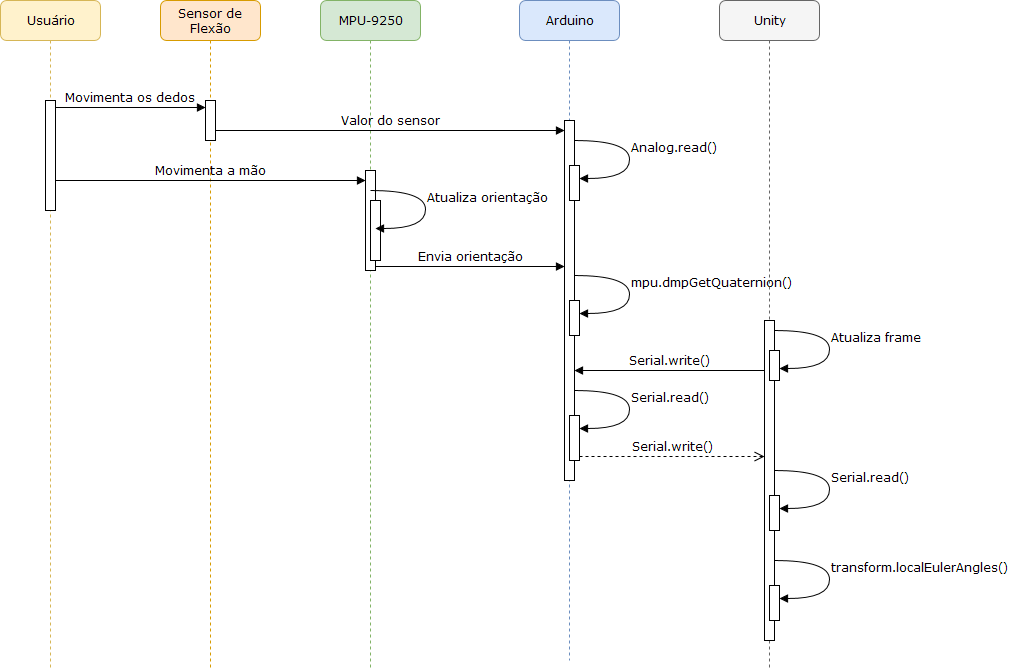
\includegraphics[width=\textwidth]{imagem/sequencia}
  \captionsetup{justification=centering}
  \captionfont{\small{\textbf{\\Fonte: Elaborado pelo Autor}}}
  \label{fig:seq}
\end{figure}

\section{Requisitos}
\label{sec:requisitos}
Os requisitos foram definidos com o intuito de definir o escopo do trabalho, prover uma base para realização de testes e ajudar a verificar o funcionamento correto do dispositivo, quando concluído.

Os requisitos de \textit{hardware} para este projeto são:

\begin{compactitem}
  \item[a)] detectar os movimentos de adução e abdução dos dedos de $\pm$ \ang{15};
  \item[b)] detectar os movimentos de desvio radial e ulnar do pulso de $\pm$ \ang{20};
  \item[c)] nenhum componente da luva poderá impedir algum movimento da mão usuário.
\end{compactitem}

A escolha dos valores dos ângulos de abdução e desvio radial e ulnar do pulso foram baseadas nos limites dos movimentos da mão humana (\cite{hand_motions}).

Os requisitos de \textit{software} para este projeto são:

\begin{compactitem}
  \item[a)] reprodução dos movimentos dos dedos do usuário pelo modelo \ac{3D};
  \item[b)] rotação do modelo \ac{3D} de acordo com a orientação da mão do usuário;
  \item[c)] movimentos suaves do modelo \ac{3D}.
\end{compactitem}

\section{\textit{Hardware}}
\label{sec:hardware}

Nesta seção serão apresentados os componentes de \textit{hardware} que serão utilizados para a execução do projeto.

\subsection{Arduino}
\label{sub:arduino}
Assim como no trabalho de \citeonline{roversi}, foi mantida a plataforma \textit{Arduino} para desenvolvimento do projeto. Os principais motivos dessa escolha foram a grande quantidade disponível de módulos, \textit{shields} e sensores, e sua ativa comunidade de desenvolvimento, disponibilizando documentação e bibliotecas para estes dispositivos. Um outro fator que contribuiu para essa decisão foi a facilidade de desenvolver protótipos nessa plataforma.

Para esse projeto, optou-se por utilizar o \textit{Arduino Mega 2560}, devido ao fato de possuir a quantidade necessária de entradas analógicas para conexão com os sensores de flexão, já que serão utilizados 14 sensores e este modelo possui 16 entradas analógicas, como especificado na Tabela \ref{tab:ardspec}. A Figura \ref{fig:arduino} apresenta o \textit{Arduino Mega 2560} que foi utilizado para leitura dos dados dos sensores e comunicação com o computador.

\begin{figure}[H]
  \setlength{\abovecaptionskip}{0pt}
  \setlength{\belowcaptionskip}{0pt}
  \caption[\textit{Arduino Mega 2560}]{\textit{Arduino Mega 2560}}
  \centering
  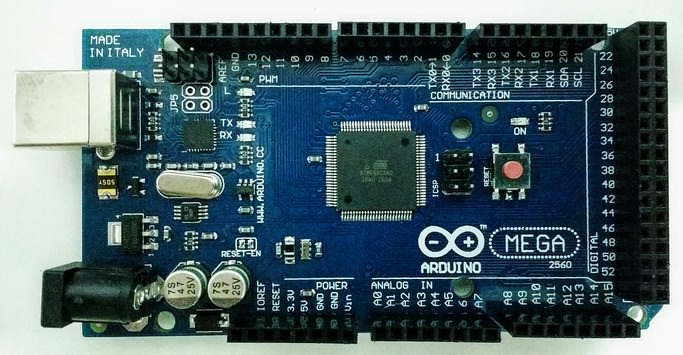
\includegraphics[width=0.5\textwidth]{imagem/ArduinoMega2560R3}
  \captionsetup{justification=centering}
  \captionfont{\small{\textbf{\\Fonte: Elaborado pelo Autor}}}
  \label{fig:arduino}
\end{figure}

\begin{table}[H]
  \centering
  \footnotesize
  \setlength{\abovecaptionskip}{0pt}
  \setlength{\belowcaptionskip}{0pt}
  \caption[Especificações do \textit{Arduino Mega 2560}]{Especificações do \textit{Arduino Mega 2560}}
  \label{tab:ardspec}
  \begin{tabular}{l l}
    \hline\hline
    Microcontrolador                & ATmega2560 \\
    Tensão de Operação              & \SI{5}{\volt} \\
    Tensão de entrada (recomendada) & \SIrange[range-phrase = --]{7}{12}{\volt} \\
    Tensão de entrada (limite)      & \SIrange[range-phrase = --]{6}{20}{\volt} \\
    Pinos de E/S Digital            & 54 (15 com saída PWM) \\
    Pinos de Entrada Analógica      & 16 \\
    Corrente DC por Pino de E/S     & \SI{20}{\milli\ampere} \\
    Corrente DC por Pino 3.3V       & \SI{50}{\milli\ampere} \\
    Memória \textit{Flash}          & \SI{256}{\kilo\byte} (\SI{8}{\kilo\byte} utilizados pelo \textit{bootloader}) \\
    SRAM                            & \SI{8}{\kilo\byte} \\
    EEPROM                          & \SI{4}{\kilo\byte} \\
    \textit{Clock}                  & \SI{16}{\mega\hertz} \\
    Comprimento                     & \SI{101.52}{\mm} \\
    Largura                         & \SI{53.3}{\mm} \\
    Peso                            & \SI{37}{\gram} \\
    \hline\hline
  \end{tabular}
  \\\vspace{1.3mm}
  \captionfont{\small{\textbf{Fonte: \citeonline{arduino}}}}
\end{table}

\subsection{Sensor Flexão}
\label{sub:sensorflexão}
Para a leitura dos movimentos dos dedos, optou-se por continuar a utilizar o sensor de flexão de 2.2" da \textit{Spectra Symbol}, devido ao fato de ser leve, não intrusivo para o usuário, simples de utilizar e fornecer resultados satisfatórios. A Figura \ref{fig:spectraflex} apresenta o sensor de flexão utilizado e a Tabela \ref{tab:flexspec} mostra suas especificações técnicas.

Foram utilizados 14 sensores, sendo dois sensores por dedo para captar os movimentos de flexão e extensão e 4 sensores entre cada dedo, detectando movimentos de adução e abdução. A disposição dos sensores na luva está representada na Figura \ref{fig:novaluva}. Foi utilizado apenas um sensor para detectar as dobras da segunda e terceira falanges para simplificar a construção da luva e reduzir custos. O ângulo de dobra da terceira falange pode ser calculado a partir do ângulo de de dobra da segunda falange (\cite{li2009smartglove}).

\begin{table}[H]
  \centering
  \footnotesize
  \setlength{\abovecaptionskip}{0pt}
  \setlength{\belowcaptionskip}{0pt}
  \caption[Especificações do Sensor de Flexão]{Especificações do Sensor de Flexão}
  \label{tab:flexspec}
  \begin{tabular}{l l}
    \hline\hline
    Ciclo de vida             & > 1 milhão \\
    Altura                    & \SI{0.43}{\mm} \\
    Comprimento ativo         & \SI{55.37}{\mm} \\
    Largura                   & \SI{6.35}{\mm} \\
    Variação de temperatura   & \SIrange{-35}{+80}{\degreeCelsius} \\
    Resistência plano         & \SI{25}{\kilo\ohm} \\
    Tolerância da resistência & \SI{+-30}{\percent} \\
    Variação de Resistência   & \SIrange{45}{125}{\kilo\ohm} (depende do raio de dobra) \\
    Potência                  & \SI{0.50}{\watt} contínuos. Pico \SI{1}{\watt} \\
    \hline\hline
  \end{tabular}
  \\\vspace{1.3mm}
  \captionfont{\small{\textbf{Fonte: \citeonline{symbol2012flex}}}}
\end{table}

\begin{figure}[H]
  \setlength{\abovecaptionskip}{0pt}
  \setlength{\belowcaptionskip}{0pt}
  \caption[Sensor de Flexão Spectra Symbol]{Sensor de Flexão Spectra Symbol}
  \centering
  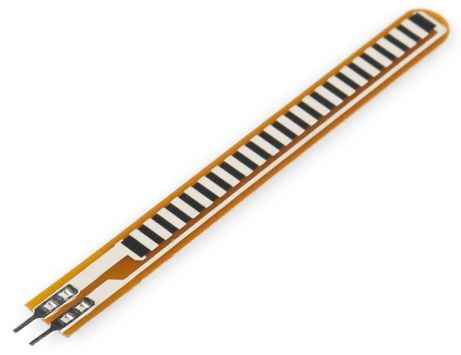
\includegraphics[width=0.4\textwidth]{imagem/spectraFlex}
  \captionsetup{justification=centering}
  \captionfont{\small{\textbf{\\Fonte: \citeonline{sparkflex}}}}
  \label{fig:spectraflex}
\end{figure}

\subsection{\ac{IMU}}
\label{sub:mpu}
Para a leitura da orientação da mão, foi utilizado a \ac{IMU} \textit{MPU-9250} da \textit{InvenSense} (Figura \ref{fig:mpu9250}). A escolha dessa \ac{IMU} deu-se primariamente pelo fato de ser acessível e possuir 9 \ac{DOF}, ou seja, consegue detectar movimentos de translação e rotação sobre qualquer um dos três eixos do espaço com maior precisão, fazendo uso de um acelerômetro, um giroscópio e um magnetômetro. Como especificado na Tabela \ref{tab:mpuspec}, o circuito do \textit{MPU-9250} possui comunicação através do protocolo \ac{I2C}, tornando sua utilização simples e permitindo a conexão de dois ou mais \ac{IMU} com apenas duas conexões (\ac{SDA} e \ac{SCL}) no \textit{Arduino}.

Foi utilizada a biblioteca \textit{I\textsuperscript{2}Cdevlib} \cite{i2c}, que possui funções para comunicação com diversos dispositivos que utilizam a interface I\textsuperscript{2}C (\ac{I2C}), como a \ac{IMU} em questão. Essa biblioteca possibilita a ativação e utilização do \ac{DMP} do \textit{MPU-9250}, que faz operações matemáticas complexas para combinar as leituras do acelerômetro, giroscópio e magnetômetro sem a utilização do processador do \textit{Arduino}, e fornecer dados confiáveis e livres de ruído que serão utilizados para calcular a orientação da \ac{IMU} no espaço.

\begin{figure}[H]
  \setlength{\abovecaptionskip}{0pt}
  \setlength{\belowcaptionskip}{0pt}
  \caption[\ac{IMU} MPU-9250]{\ac{IMU} MPU-9250}
  \centering
  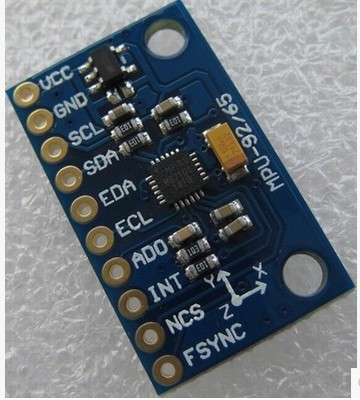
\includegraphics[height=5cm]{imagem/mpu9250}
  \captionsetup{justification=centering}
  \captionfont{\small{\textbf{\\Fonte: \citeonline{mpu9250}}}}
  \label{fig:mpu9250}
\end{figure}

\begin{table}[H]
  \centering
  \footnotesize
  \setlength{\abovecaptionskip}{0pt}
  \setlength{\belowcaptionskip}{0pt}
  \caption[Especificações do IMU \textit{MPU-9250}]{Especificações do IMU \textit{MPU-9250}}
  \label{tab:mpuspec}
  \begin{tabular}{l l}
    \hline\hline
    Tensão de operação (VDD)    & \SIrange[range-phrase = --]{2.4}{3.6}{\volt} \\
    Tensão lógica (VDDIO)       & \SI{1.7}{\volt} a VDD, ou VDD \\
    Saída Digital               & I\textsuperscript{2}C / SPI \\
    Sensibilidade Acelerômetro  & \SI[per-mode=fraction]{+-4800}{LSB\per\g} \\
    Gama Acelerômetro           & \SI{+-2}, \SI{+-4}, \SI{+-8}, \SI{+-16}{LSB\per\g} \\
    Taxa de Ruído do Giroscópio & \SI{+-4800}{\micro\farad} \\
    Gama Giroscópio             & \SI{+-250}, \SI{+-500}, \SI{+-1000}, \SI[per-mode=symbol]{+-2000}{\degree\per\second} \\
    Dimensões do Componente   & \SI[product-units = single]{3 x 3 x 1}{\mm}\\
    \hline\hline
  \end{tabular}
  \\\vspace{1.3mm}
  \captionfont{\small{\textbf{Fonte: \citeonline{specmpu9250}}}}
\end{table}

\subsection{Circuito}
\label{sub:circuito}
O Apêndice \ref{apend:circ} apresenta o diagrama elétrico completo do circuito do projeto. Como mostrado na Tabela \ref{tab:listacomponentes} foram utilizados 14 sensores de flexão que estão conectados às entradas analógicas do \textit{Arduino} como mostra a Figura \ref{fig:circsens}, com 14 resistores de \SI{10}{\kilo\ohm} fazendo um divisor de tensão para obter os dados dos sensores. De acordo com a Figura \ref{fig:circimu}, as duas \ac{IMU}s foram conectadas nos pinos \ac{SCL} e \ac{SDA} da interface \ac{I2C} e, seus pinos \ac{INT} conectados aos pinos digitais 2 e 3 do \textit{Arduino} que são os pinos 6 e 7 do \textit{ATmega 2560}, representados na Figura \ref{fig:circard}. Os pinos AD0 das \ac{IMU}s foram conectados em \SI{3.3}{\volt} e \ac{GND} para que possam ter endereços diferentes no barramento \ac{I2C}. A comunicação entre o computador e o \textit{Arduino} foi feita através de um cabo \ac{USB}.

\begin{table}[H]
  \centering
  \footnotesize
  \setlength{\abovecaptionskip}{0pt}
  \setlength{\belowcaptionskip}{0pt}
  \caption[Lista de Componentes]{Lista de Componentes}
  \label{tab:listacomponentes}
  \begin{tabular}{l r}
    \hline\hline
    \multicolumn{1}{c}{Componente}&\multicolumn{1}{c}{Quantidade}\\
    \hline
    \textit{Arduino Mega}           & 1 \\
    \textit{MPU-9250}               & 2 \\
    Conectores em barra de 40 pinos & 1 \\
    \textit{Shield} de Prototipagem para \textit{Arduino} & 1 \\
    Sensores de flexão              & 14 \\
    Resistores (\SI{10}{\kilo\ohm}) & 14 \\
    Fios & 40\\
    \hline\hline
  \end{tabular}
  \\\vspace{1.3mm}
  \captionfont{\small{\textbf{Fonte: Elaborado pelo Autor}}}
\end{table}

\begin{figure}[H]
  \setlength{\abovecaptionskip}{0pt}
  \setlength{\belowcaptionskip}{0pt}
  \caption[Detalhes do circuito elétrico]{Detalhes do circuito elétrico}
  \centering
  \subfloat[Conexões Sensores]{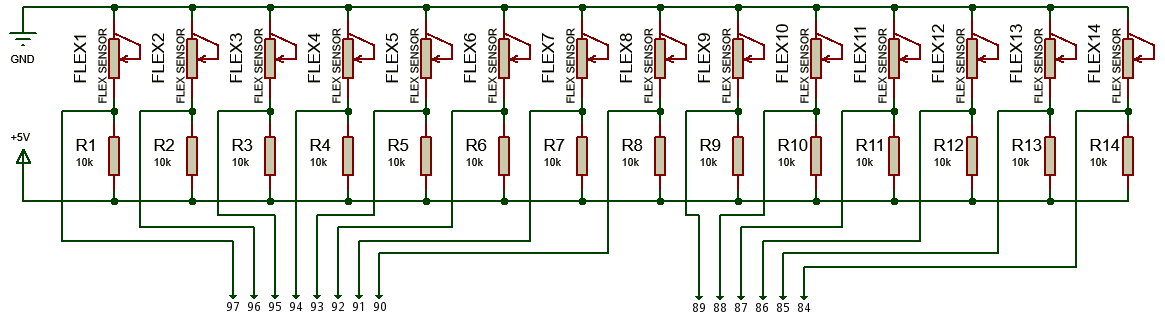
\includegraphics[width=\textwidth]{imagem/ProteusLuvaSensores}\label{fig:circsens}}\\
  \subfloat[Conexões \textit{Arduino}]{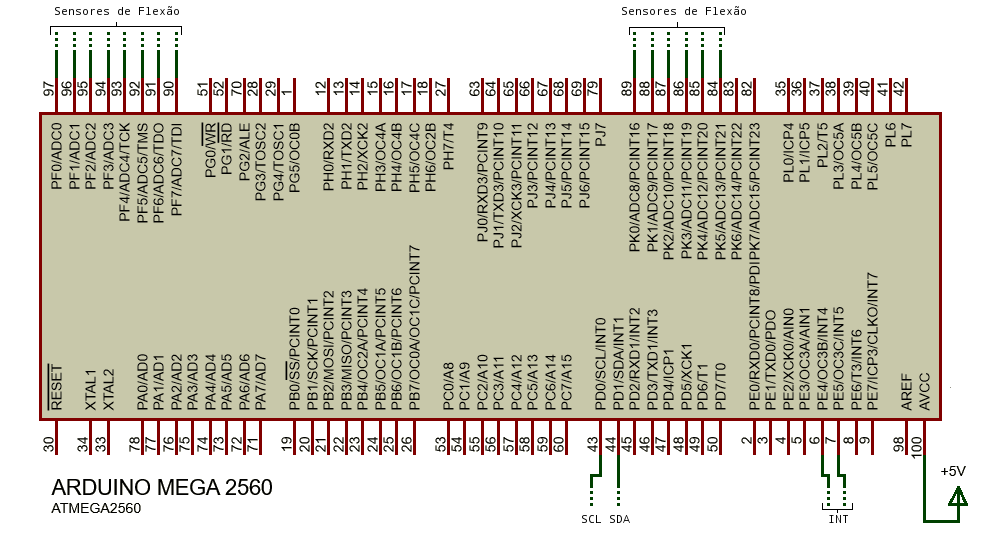
\includegraphics[width=\textwidth]{imagem/ProteusLuvaArduino}\label{fig:circard}}\\
  \label{fig:circLuva1}
  \captionsetup{justification=centering}
  \captionfont{\small{\textbf{\\Fonte: Elaborado pelo Autor}}}
\end{figure}

\begin{figure}[H]
\ContinuedFloat
  \setlength{\abovecaptionskip}{0pt}
  \setlength{\belowcaptionskip}{0pt}
  \caption[Detalhes do circuito elétrico]{Detalhes do circuito elétrico}
  \centering
  \subfloat[Conexões \ac{IMU}s]{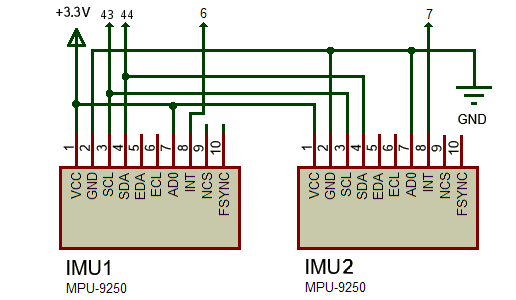
\includegraphics[width=.5\textwidth]{imagem/ProteusLuvaIMU}\label{fig:circimu}}\\
  \label{fig:circLuva2}
  \captionsetup{justification=centering}
  \captionfont{\small{\textbf{\\Fonte: Elaborado pelo Autor}}}
\end{figure}

\section{\textit{Software}}
\label{sec:software}

Nesta seção serão apresentados os \textit{softwares} que foram utilizados para a execução do projeto.

\subsection{Unity}
\label{sub:unity}
Para animação e exibição do modelo \ac{3D}, optou-se pela utilização da plataforma \textit{Unity}, versão 5.6.2, que é um ambiente para desenvolvimento para jogos digitais. A escolha dessa plataforma deu-se com base em sua facilidade de aprendizado e utilização, e também na grande variedade de modelos \ac{3D} disponibilizados por sua comunidade.

O modelo de mão e braço \ac{3D} utilizado foi o mesmo de \citeonline{roversi} (Figura \ref{fig:maounity}). Para a movimentação do modelo, foi implementado um \textit{script} em \csharp que recebe os dados de cada sensor provenientes do \textit{Arduino} e aplica as transformações dos dedos e na rotação da mão \ac{3D}.

A aplicação \textit{Unity} exibe a representação da mão do usuário em um modelo \ac{3D} que replica os movimentos realizados.

\begin{figure}[H]
  \setlength{\abovecaptionskip}{0pt}
  \setlength{\belowcaptionskip}{0pt}
  \caption[Tela da aplicação Unity]{Tela da aplicação Unity}
  \centering
  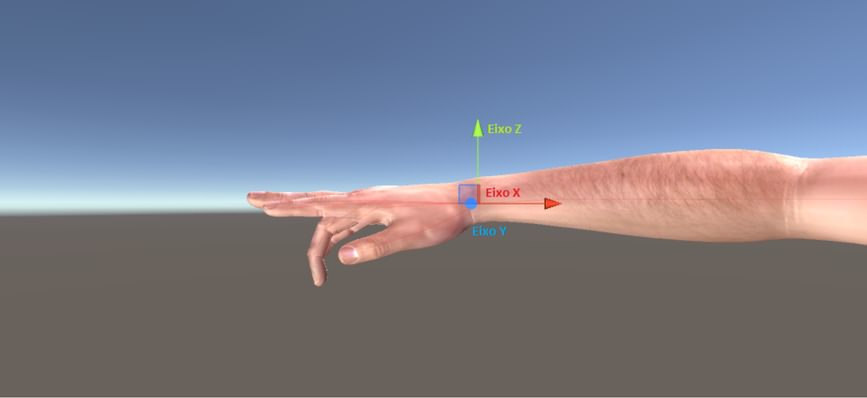
\includegraphics[trim=40 20 40 20,clip,width=.5\textwidth]{imagem/maoUnity}
  \captionsetup{justification=centering}
  \captionfont{\small{\textbf{\\Fonte: \citeonline{roversi}}}}
  \label{fig:maounity}
\end{figure}

\section{Plataforma de Desenvolvimento}
\label{sub:plataforma_de_desenvolvimento}
Este trabalho foi desenvolvido em um \textit{notebook} \textit{HP}, modelo \textit{G71}. Suas especificações são mostradas na Tabela \ref{tab:especificacoes} abaixo:

\begin{table}[H]
  \centering
  \footnotesize
  \setlength{\abovecaptionskip}{0pt}
  \setlength{\belowcaptionskip}{0pt}
  \caption[Especificações da plataforma de desenvolvimento]{Especificações da plataforma de desenvolvimento}
  \label{tab:especificacoes}
    \begin{tabular}{l l}
    \hline\hline
    Processador         & \textit{Intel Core 2 Duo T6600} \SI{2.20}{\giga\hertz} \\
    Memória             & \SI{4}{\giga\byte}\\
    Placa de vídeo      & \textit{Intel Graphics Media Accelerator 4500MHD} \\
    Disco Rígido        & \SI{320}{\giga\byte} (5400RPM) \\
    Sistema Operacional & \textit{Windows 10} \SI{64}{\bit} \\
    \hline\hline
  \end{tabular}
  \\\vspace{1.3mm}
  \captionfont{\small{\textbf{Fonte: Elaborado pelo Autor}}}
\end{table}

\subsection{Casos de Teste}
\label{sub:testes}

Para a comparação dos dois protótipos, foi utilizada uma abordagem semelhante à de \citeonline{li2009smartglove}, onde foram realizadas uma série de medições do ângulo de dobra real dos dedos e comparada com o valor lido pelo sensor após as devidas conversões. A precisão dos resultados foi avaliada utilizando \ac{DMA} dado pela Equação \ref{eq:dma}: 

\begin{equation} \label{eq:dma}
	DMA = \frac{1}{n}\sum_{i=1}^n\lvert V_r - V_c \rvert
\end{equation}

Onde $n$ é o número de amostras, $V_r$ é o valor real do ângulo de dobra e $V_c$ é o valor do ângulo calculado pelo \textit{Arduino}. Idealmente os valores medidos e calculados deveriam ser iguais, ou seja, $V_r=V_c$, fazendo com que $DMA=0$, mas devido às imprecisões tanto nos sensores, quanto no processo de conversão, isso não ocorre. Portanto é desejável que o valor do \ac{DMA} seja o mais próximo de $0$.

O novo protótipo também foi analisado a fim de verificar se as seguintes falhas existentes no protótipo original foram corrigidas:

\begin{compactitem}
  \item[a)] sensores de flexão saíam de suas posições;
  \item[b)] ruídos dos sensores de flexão;
  \item[c)] ruídos do acelerômetro;
  \item[d)] comunicação ineficiente entre \textit{Arduino} e \textit{Unity}.
\end{compactitem}

A bateria de testes foi composta de nove posições, descritas a seguir, realizadas com o objetivo de analisar cada uma das articulações dos dedos (Figura \ref{fig:art}). As posições 1--4 estão representados na Figura \ref{fig:pos1}, e as posições 5--9 estão representadas na Figura \ref{fig:pos2}. Cada posição foi mantida por 10 segundos e repetida três vezes de modo a obter os valores médios do \ac{DP}, \ac{DMA} e amplitude para cada sensor. O número de repetições e a duração de cada posição foram escolhidos com base no trabalho de \citeonline{li2009smartglove}.

\begin{compactitem}
  \item[1)] extensão e adução de todos os dedos e mão plana;
  \item[2)] flexão das articulações do \ac{MCF} e \ac{IF} do polegar;
  \item[3)] flexão das articulações \ac{MCF};
  \item[4)] flexão das articulações \ac{IFP};
  \item[5)] flexão do pulso;
  \item[6)] extensão do pulso;
  \item[7)] desvio radial do pulso;
  \item[8)] desvio ulnar do pulso.
  \item[9)] abdução dos dedos.
\end{compactitem}

\begin{figure}[H]
  \setlength{\abovecaptionskip}{0pt}
  \setlength{\belowcaptionskip}{0pt}
  \caption[Articulações dos dedos]{Articulações dos dedos}
  \centering
  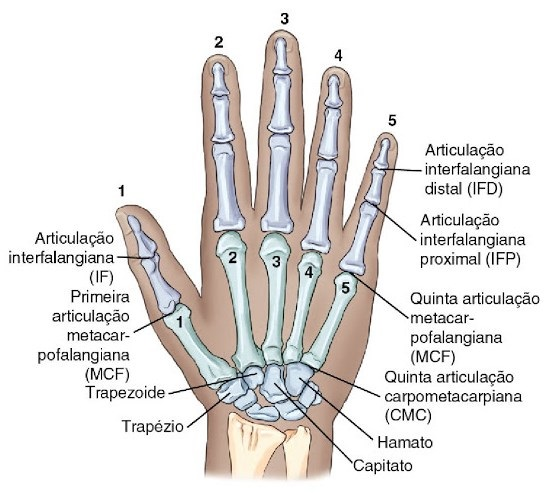
\includegraphics[width=.55\textwidth]{imagem/articulacoes}
  \captionsetup{justification=centering}
  \captionfont{\small{\textbf{\\Fonte: \citeonline{articulacoes}}}}
  \label{fig:art}
\end{figure}

\begin{figure}[H]
  \setlength{\abovecaptionskip}{0pt}
  \setlength{\belowcaptionskip}{0pt}
  \caption[Posições dos dedos para testes]{Posições dos dedos para testes}
  \centering
  \subfloat[1--4]{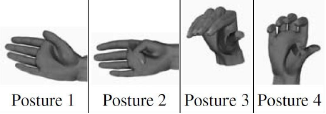
\includegraphics[width=.5\textwidth]{imagem/posicoes}\label{fig:pos1}}\\
  \subfloat[5--9]{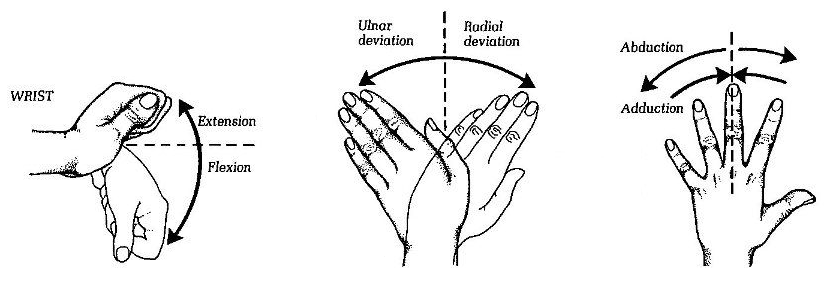
\includegraphics[width=.5\textwidth]{imagem/posicoes2}\label{fig:pos2}}
  \captionsetup{justification=centering}
  \captionfont{\small{\textbf{\\Fonte: \citeonline{li2009smartglove}, \citeonline{movimentos} (modificado pelo Autor)}}}
  \label{fig:pos}
\end{figure}

Para cada sensor e cada posição foi realizada uma análise estatística dos ângulos de dobra obtidos, calculando o \ac{DP} pela Equação \ref{eq:dp} e amplitude pela Equação \ref{eq:amp}, onde $X_S$ é o conjunto de amostras obtidas do sensor $S$ e $n$ é o número total de amostras. Por fim foi feita a média dos desvios padrão, amplitude e \ac{DMA} de cada sensor.

\begin{equation} \label{eq:dp}
	\delta_S = \sqrt{\frac{\sum_{i=1}^n(X_{S_i} - \overline{X_S})^2}{n-1}}
\end{equation}

\begin{equation} \label{eq:amp}
	R_S = \max(X_{S_i}) - \min(X_{S_i})
\end{equation}

% Nome do capítulo
\chapter{Desenvolvimento}
% Label para referenciar
\label{ch:desenvolvimento}

% Diminuir espaçamento entre título e texto
\vspace{-1.9cm}
O desenvolvimento desse trabalho se deu em duas etapas: montagem do \textit{Hardware} e implementação do \textit{Software}. Cada uma dessas etapas será descrita nas próximas seções.

\section{\textit{Hardware}} % (fold)
\label{sec:met_hardware}

Nesta etapa foi utilizada uma luva de material diferente a fim de corrigir o problema da fixação dos sensores nos dedos e para comparação dos protótipos foi elaborado um novo circuito utilizando um \textit{shield} de prototipagem para \textit{Arduino} com conectores que permitem que os sensores de flexão sejam ligados a qualquer um dos \textit{shields}.

\subsection{Luva} % (fold)
\label{sub:luva}
Na luva original de \citeonline{roversi}, os sensores de flexão desviavam muito de suas posições ideais quando se dobrava os dedos, o que causava leituras incorretas, principalmente no polegar e no dedo mínimo. Isso ocorria pelo fato da luva não ficar justa com a mão do usuário e do tecido da luva deformar com facilidade. Devido a isso, foi necessária a escolha de uma nova luva que se prendesse mais à mão do usuário e  com um tecido que não deformasse, permitindo uma melhor fixação dos sensores.

A luva escolhida, mostrada na Figura \ref{fig:luva_neoprene}, é feita de neoprene, um tipo de borracha sintética muito utilizada para equipamentos de mergulho, sendo flexível e resistente. Este material foi escolhido pela sua elasticidade, possibilitando se adaptar a diferentes tamanhos de mãos e garantindo que os sensores de flexão não se desloquem durante o uso do dispositivo.

\begin{figure}[H]
  \setlength{\abovecaptionskip}{0pt}
  \setlength{\belowcaptionskip}{0pt}
  \caption[Luva de neoprene utilizada]{Luva de neoprene utilizada}
  \centering
  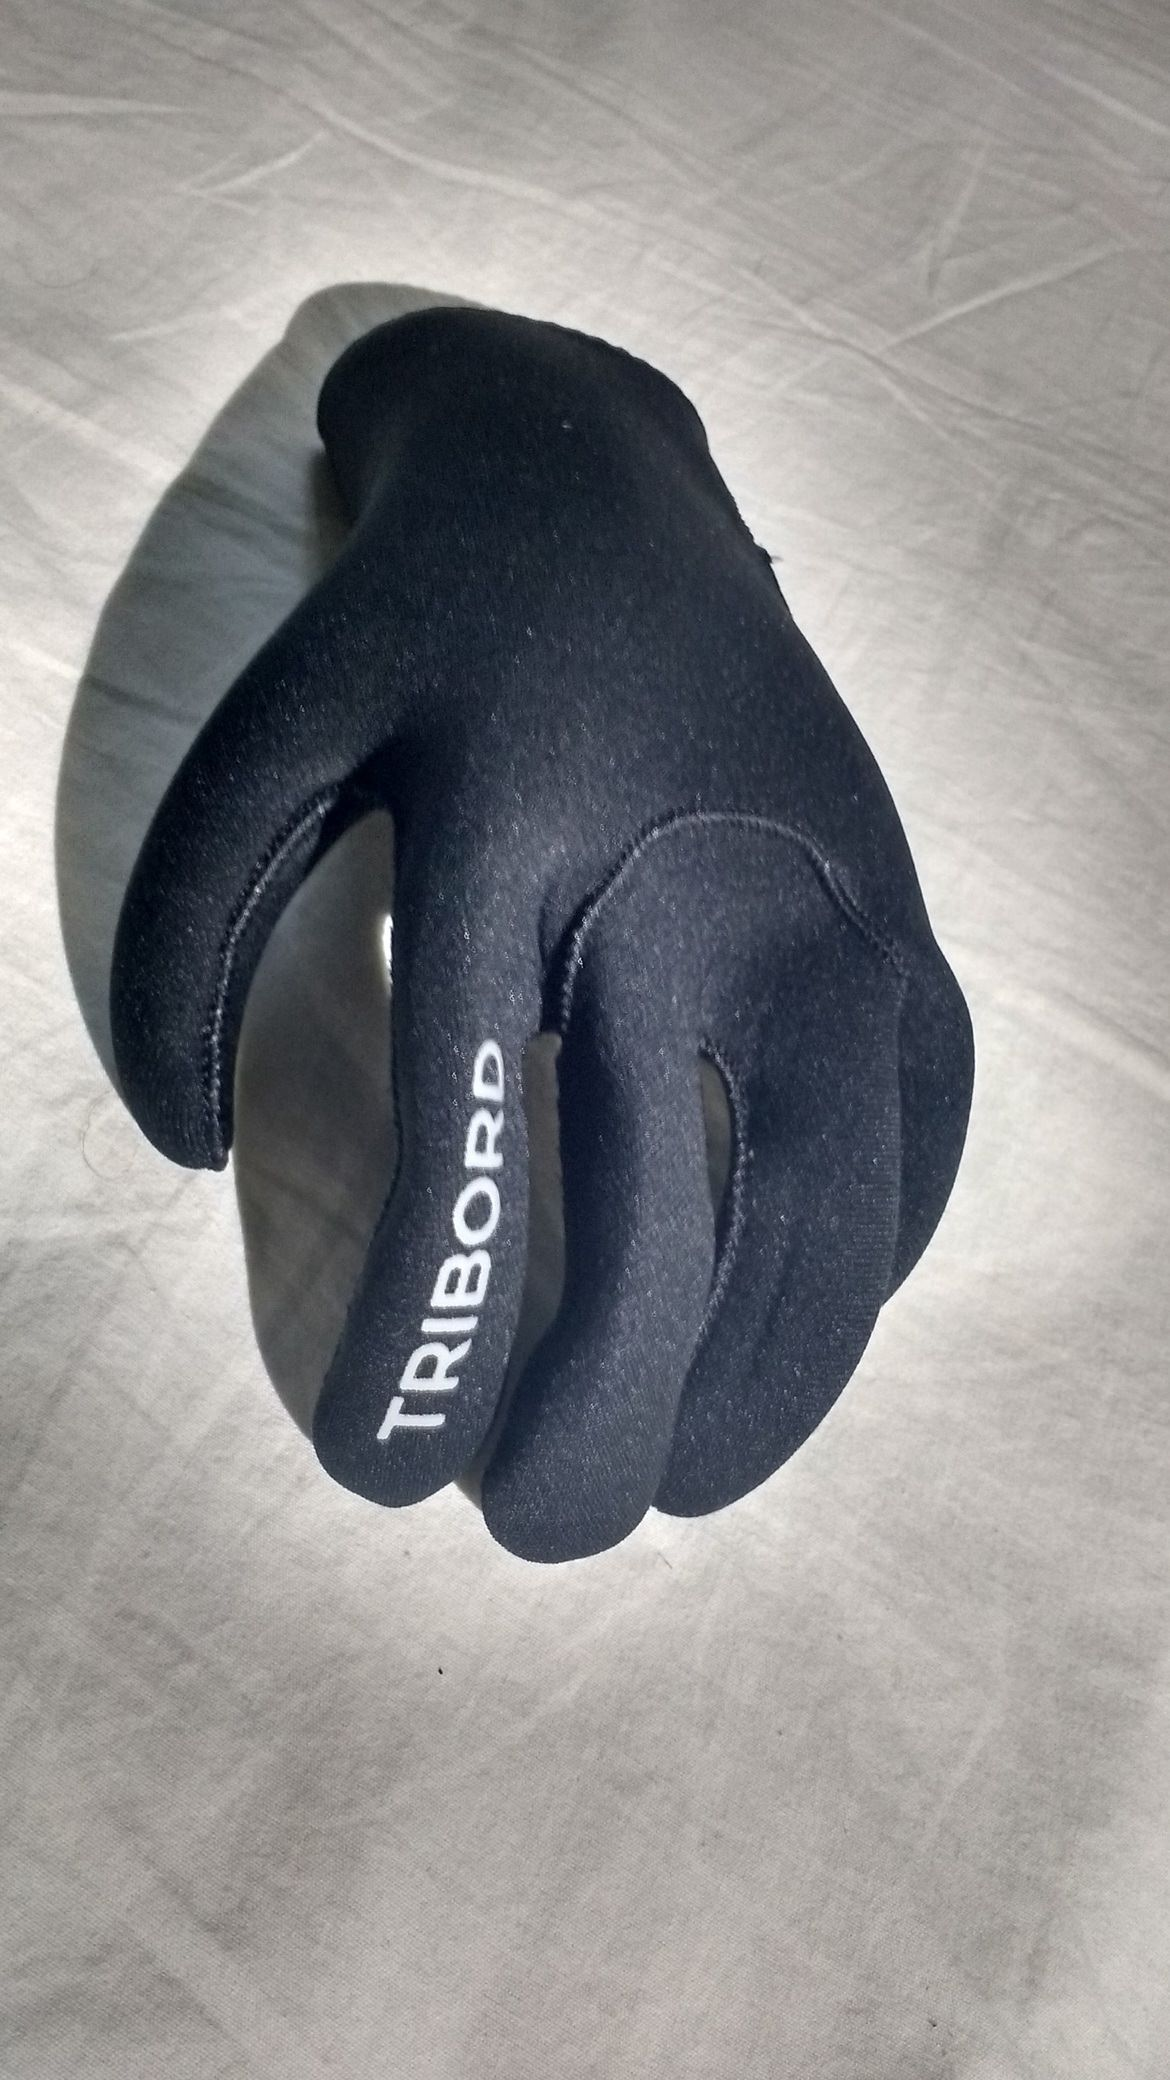
\includegraphics[trim=0 400 100 200,clip,width=.4\textwidth,angle=90]{imagem/luvaneoprene}
  \captionsetup{justification=centering}
  \captionfont{\small{\textbf{\\Fonte: Elaborado pelo Autor}}}
  \label{fig:luva_neoprene}
\end{figure}

% subsubsection luva (end)

\subsection{Sensores de Flexão} % (fold)
\label{sub:sensores_de_flexao}
Os sensores de flexão utilizados foram os mesmos do protótipo de \citeonline{roversi}, detalhados na Seção \ref{sec:sens}. Foram utilizados 14 sensores no total, sendo 5 para captar as dobras das articulações \ac{IFD} e \ac{IFP}, 5 para as articulações \ac{MCF} e 4 para detectar os movimentos de adução e abdução dos dedos. As articulações estão representadas na Figura \ref{fig:art}. Os sensores foram posicionados sobre a mão de forma que fiquem aproximadamente sobre os ossos, para garantir que eles se dobrem de maneira mais semelhante possível ao movimento que o usuário realiza.

A fixação dos sensores na luva foi feita com linha de costura na 1ª, 2ª e 3ª falange de cada dedo, para impedir que o sensor se movimente lateralmente, mas ainda consiga seguir a dobra do dedo do usuário. Para impedir que os sensores deslizem para frente ou para trás, eles também foram fixados com costura em suas bases. A Figura \ref{fig:luva_frente} apresenta os sensores na luva. Os sensores de adução e abdução foram posicionados conforme a Figura \ref{fig:novaluva} e fixados com linha de costura em suas duas extremidades. O ponto de fixação foi entre as articulações \ac{MCF} e \ac{IFP}, para que eles não dificultem os movimentos de flexão.

Ainda foi colocada uma outra luva de \textit{lycra} por cima da luva de neoprene (Figura \ref{fig:luva_lycra}) para auxiliar os sensores a dobrarem quando as articulações \ac{IFD} fossem movimentadas.

\begin{figure}[H]
  \setlength{\abovecaptionskip}{0pt}
  \setlength{\belowcaptionskip}{0pt}
  \caption[Montagem final da Luva]{Montagem final da Luva}
  \centering
  \subfloat[Sensores de flexão na luva]{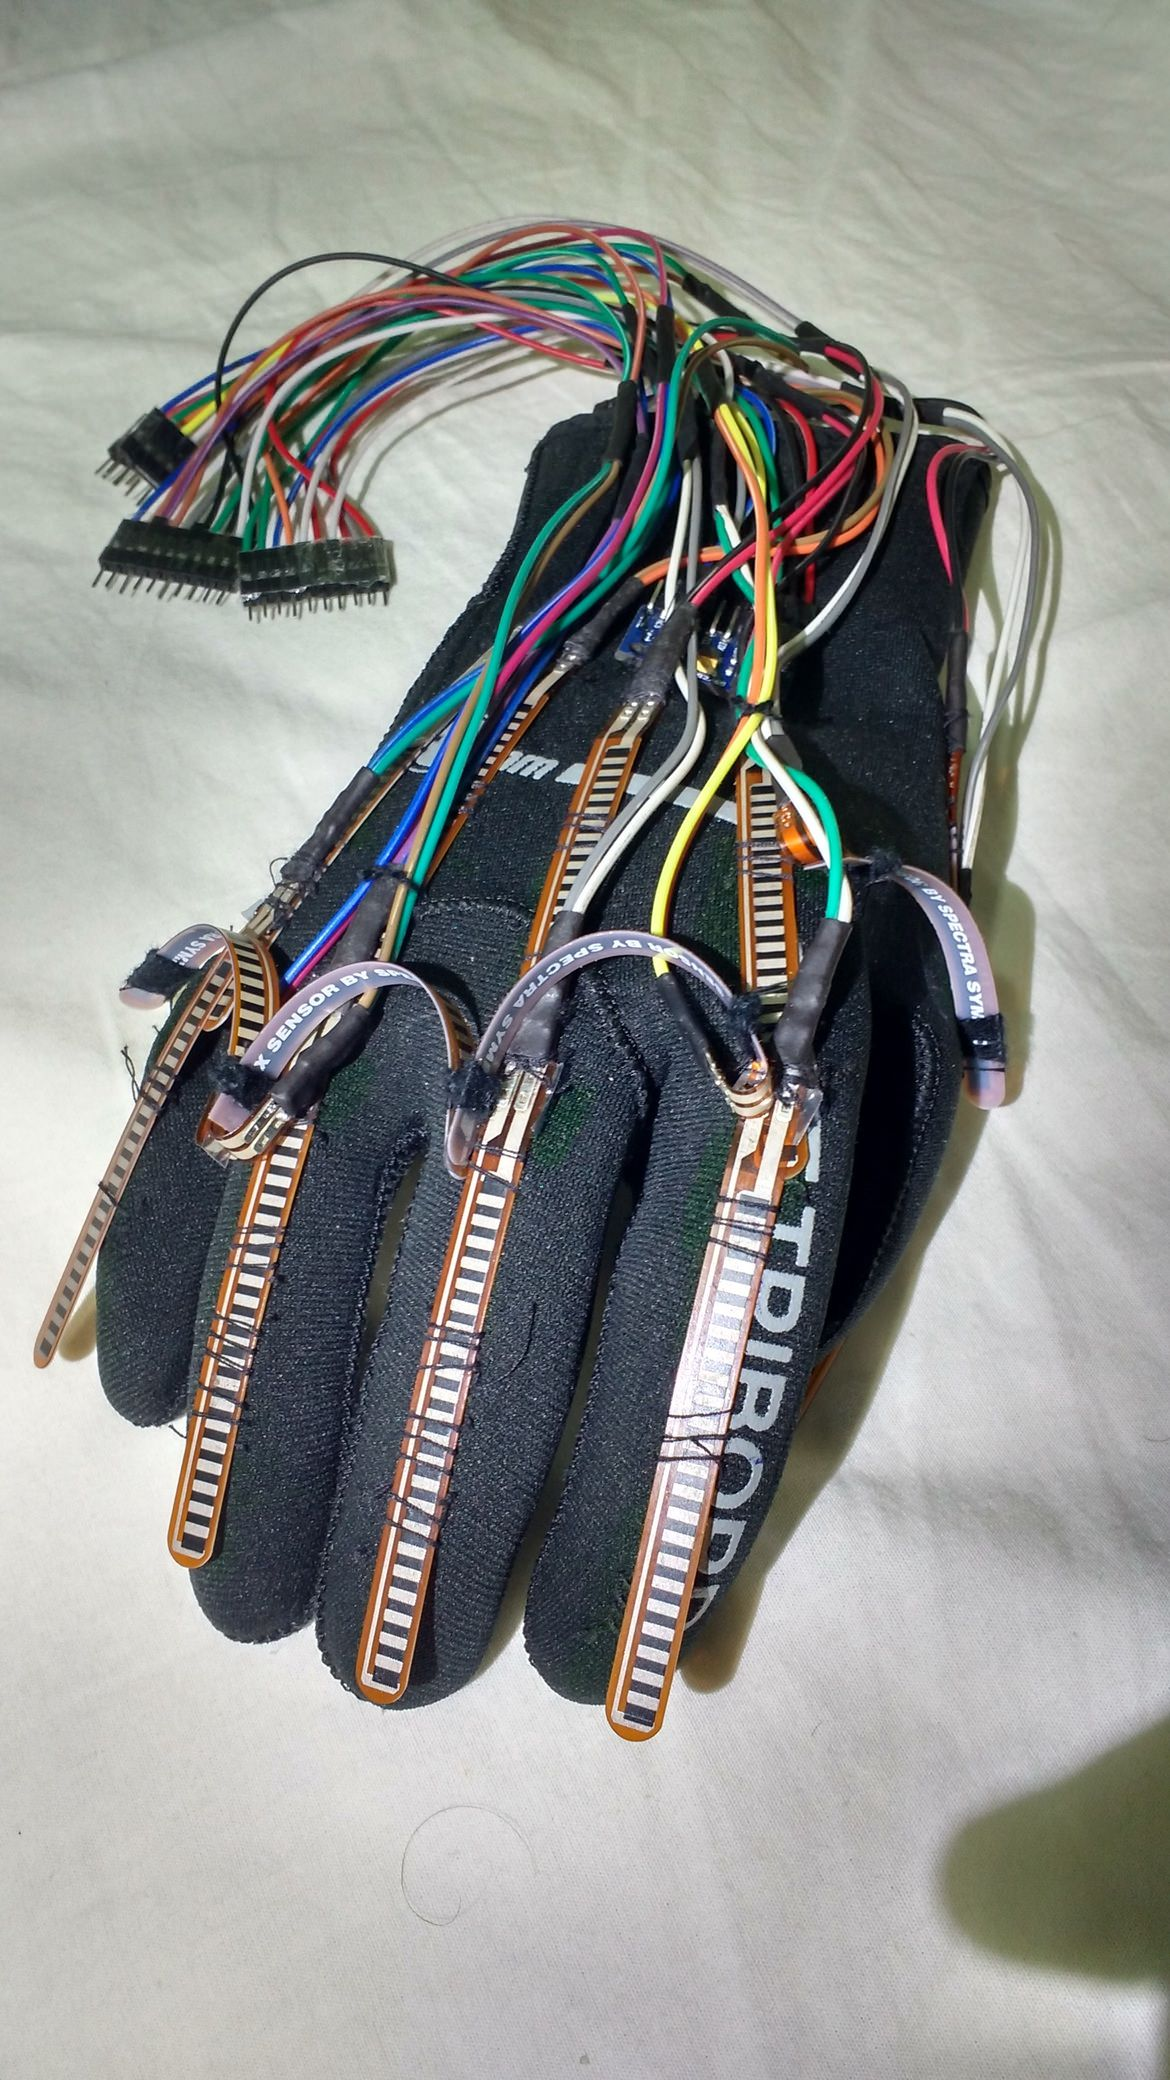
\includegraphics[trim=0 300 100 200,clip,width=.4\textwidth]{imagem/LuvaFrente}\label{fig:luva_frente}}
  \qquad
  \subfloat[Luva de \textit{lycra} cobrindo sensores]{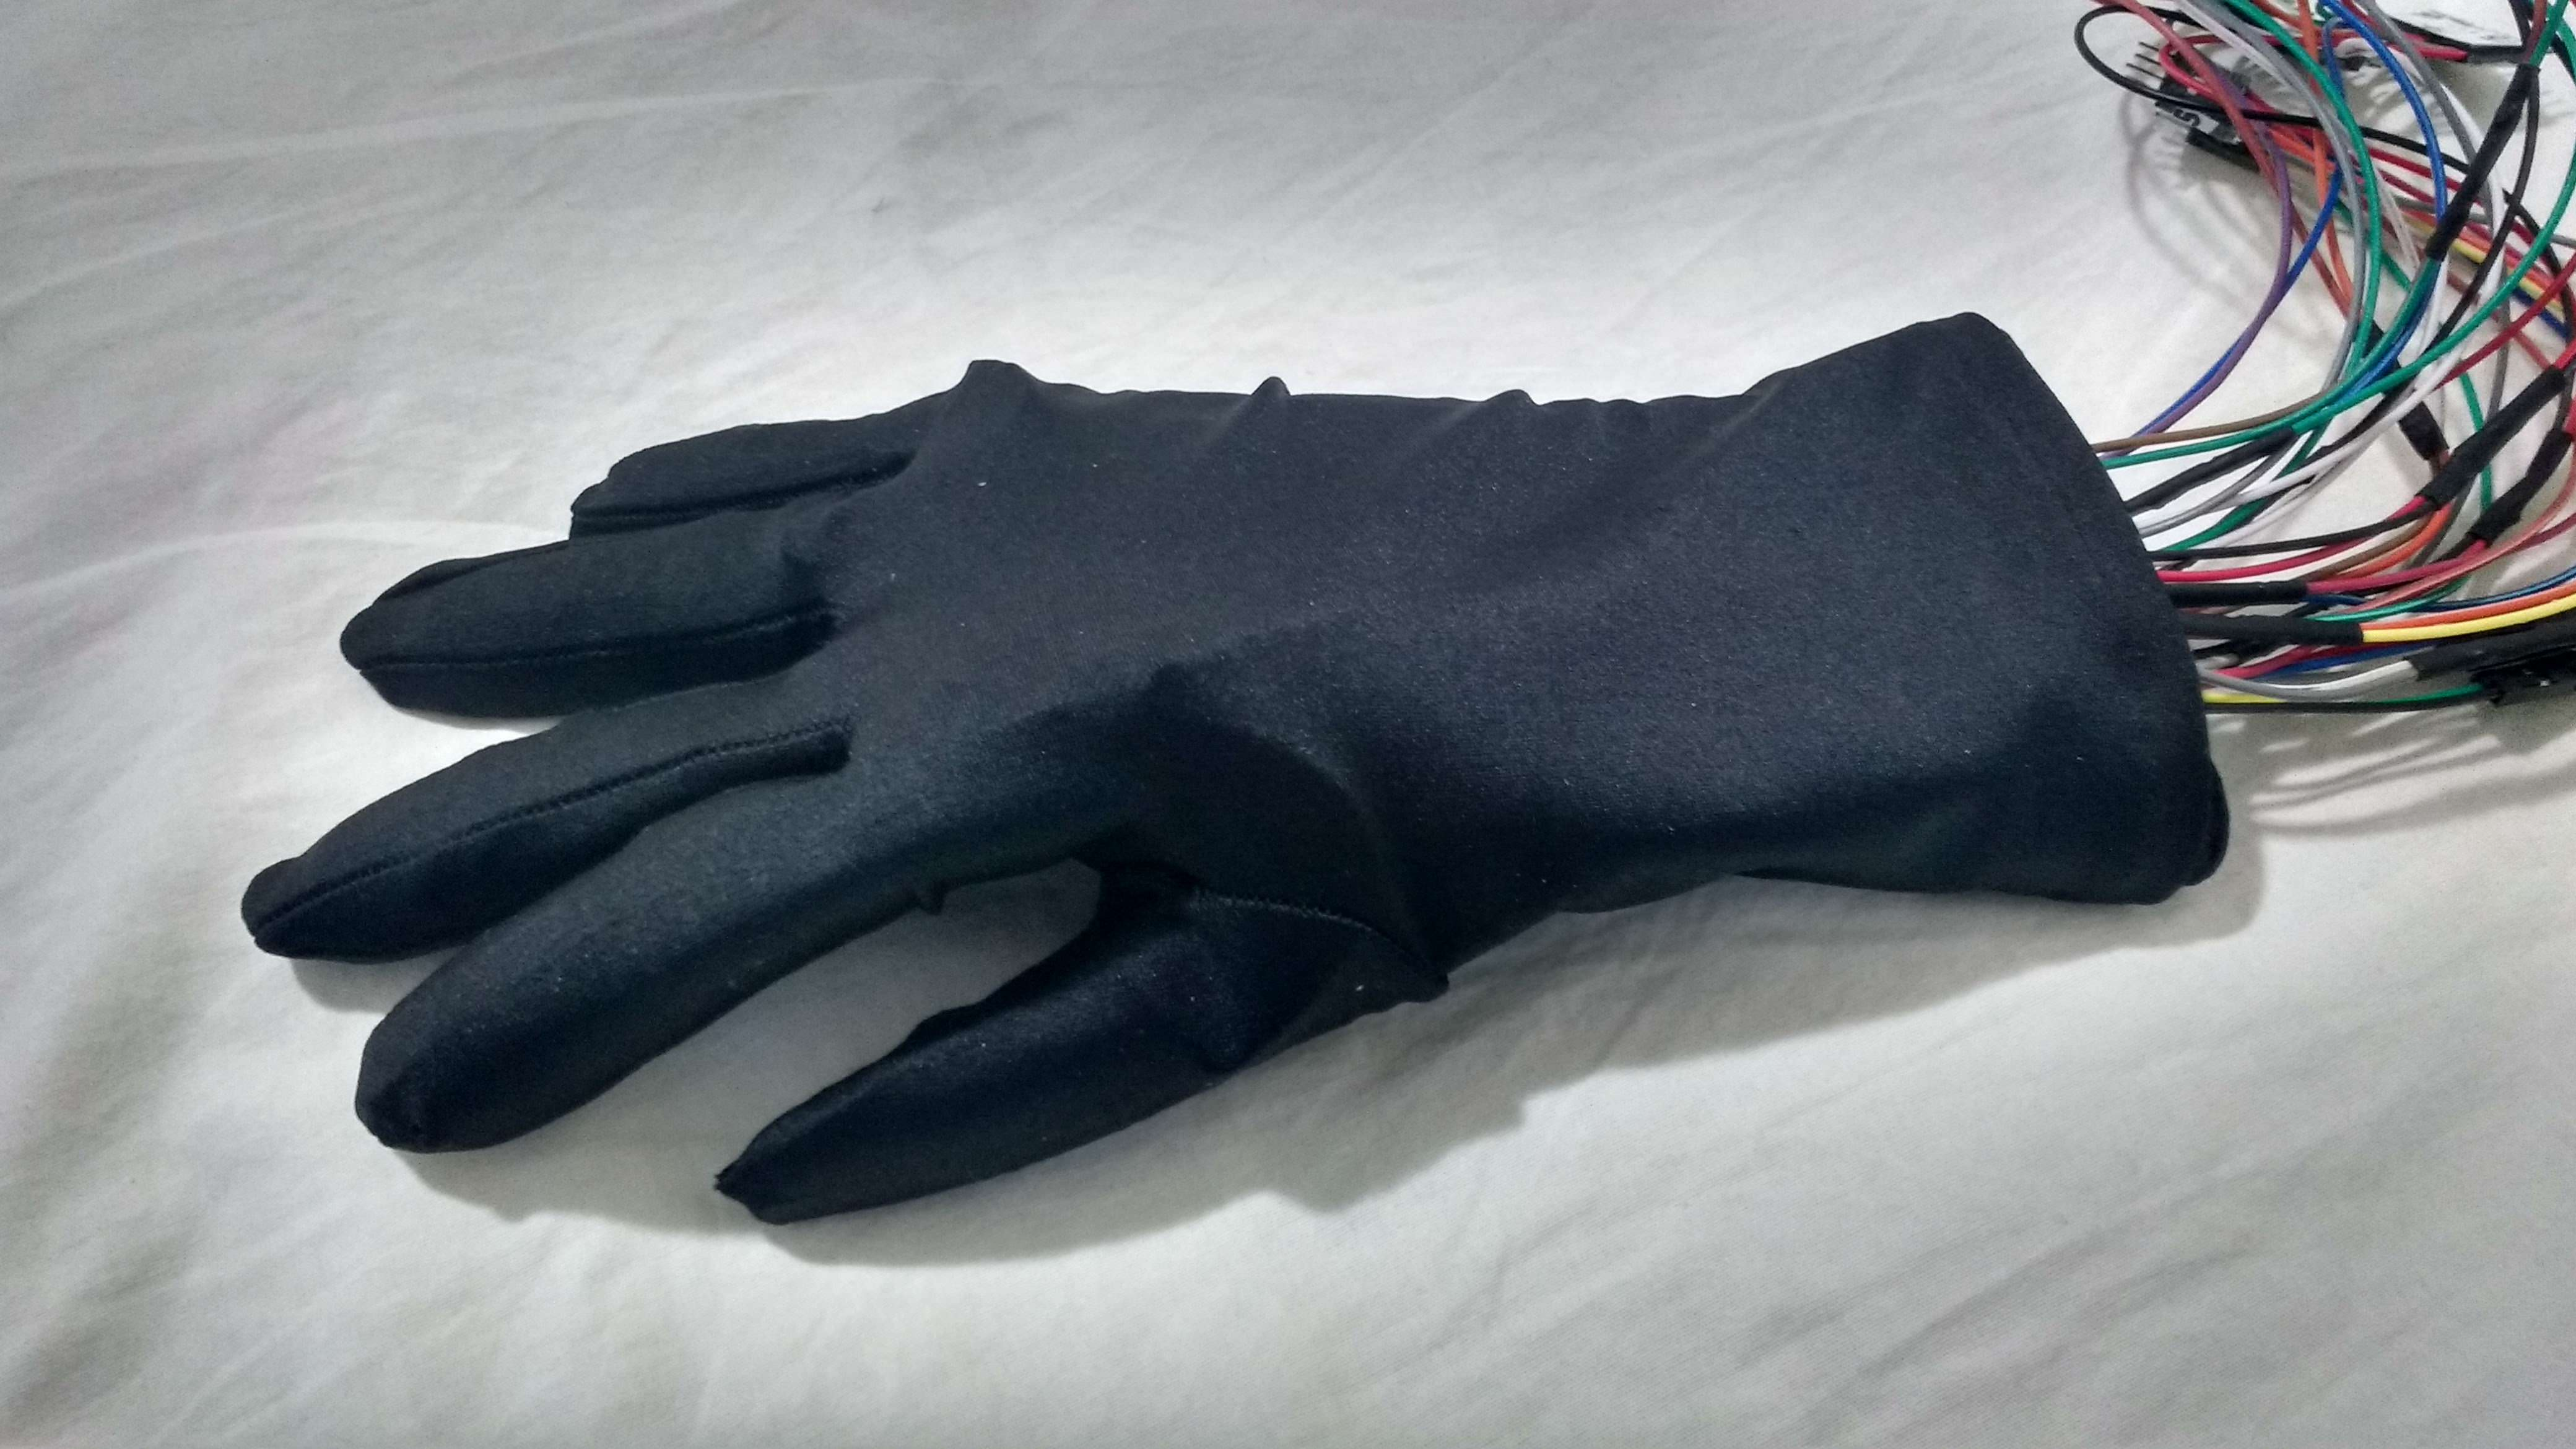
\includegraphics[width=.6\textwidth,angle =90]{imagem/luvacomlycra_mini}\label{fig:luva_lycra}}\\
  \captionsetup{justification=centering}
  \captionfont{\small{\textbf{\\Fonte: Elaborado pelo Autor}}}
  \label{fig:sensores_luva}
\end{figure}

% subsubsection sensores_de_flexão (end)

\subsection{MPU-9250} % (fold)
\label{sub:mpu_9250}
Foram utilizadas duas \ac{IMU}s \textit{MPU-9250} para conseguir obter a orientação espacial da mão. Uma \ac{IMU} foi colocada sobre as costas da mão, e a outra foi fixada no \textit{shield} de prototipagem do \textit{Arduino} que fica sobre o antebraço do usuário (Figura \ref{fig:luva_mao}). Com as \ac{IMU}s nessas posições, é possível obter os movimentos de extensão, flexão, desvio radial e ulnar do pulso. A \ac{IMU} sobre as costas da mão detecta a inclinação e rotação da mão, e a \ac{IMU} do antebraço serve como referência para o cálculo dos ângulos de dobra do pulso sobre os eixos $X$ ou $Z$ (Figura \ref{fig:maounity}).

\begin{figure}[H]
  \setlength{\abovecaptionskip}{0pt}
  \setlength{\belowcaptionskip}{0pt}
  \caption[Luva em utilização]{Luva em utilização}
  \centering
  \subfloat[Vista superior]{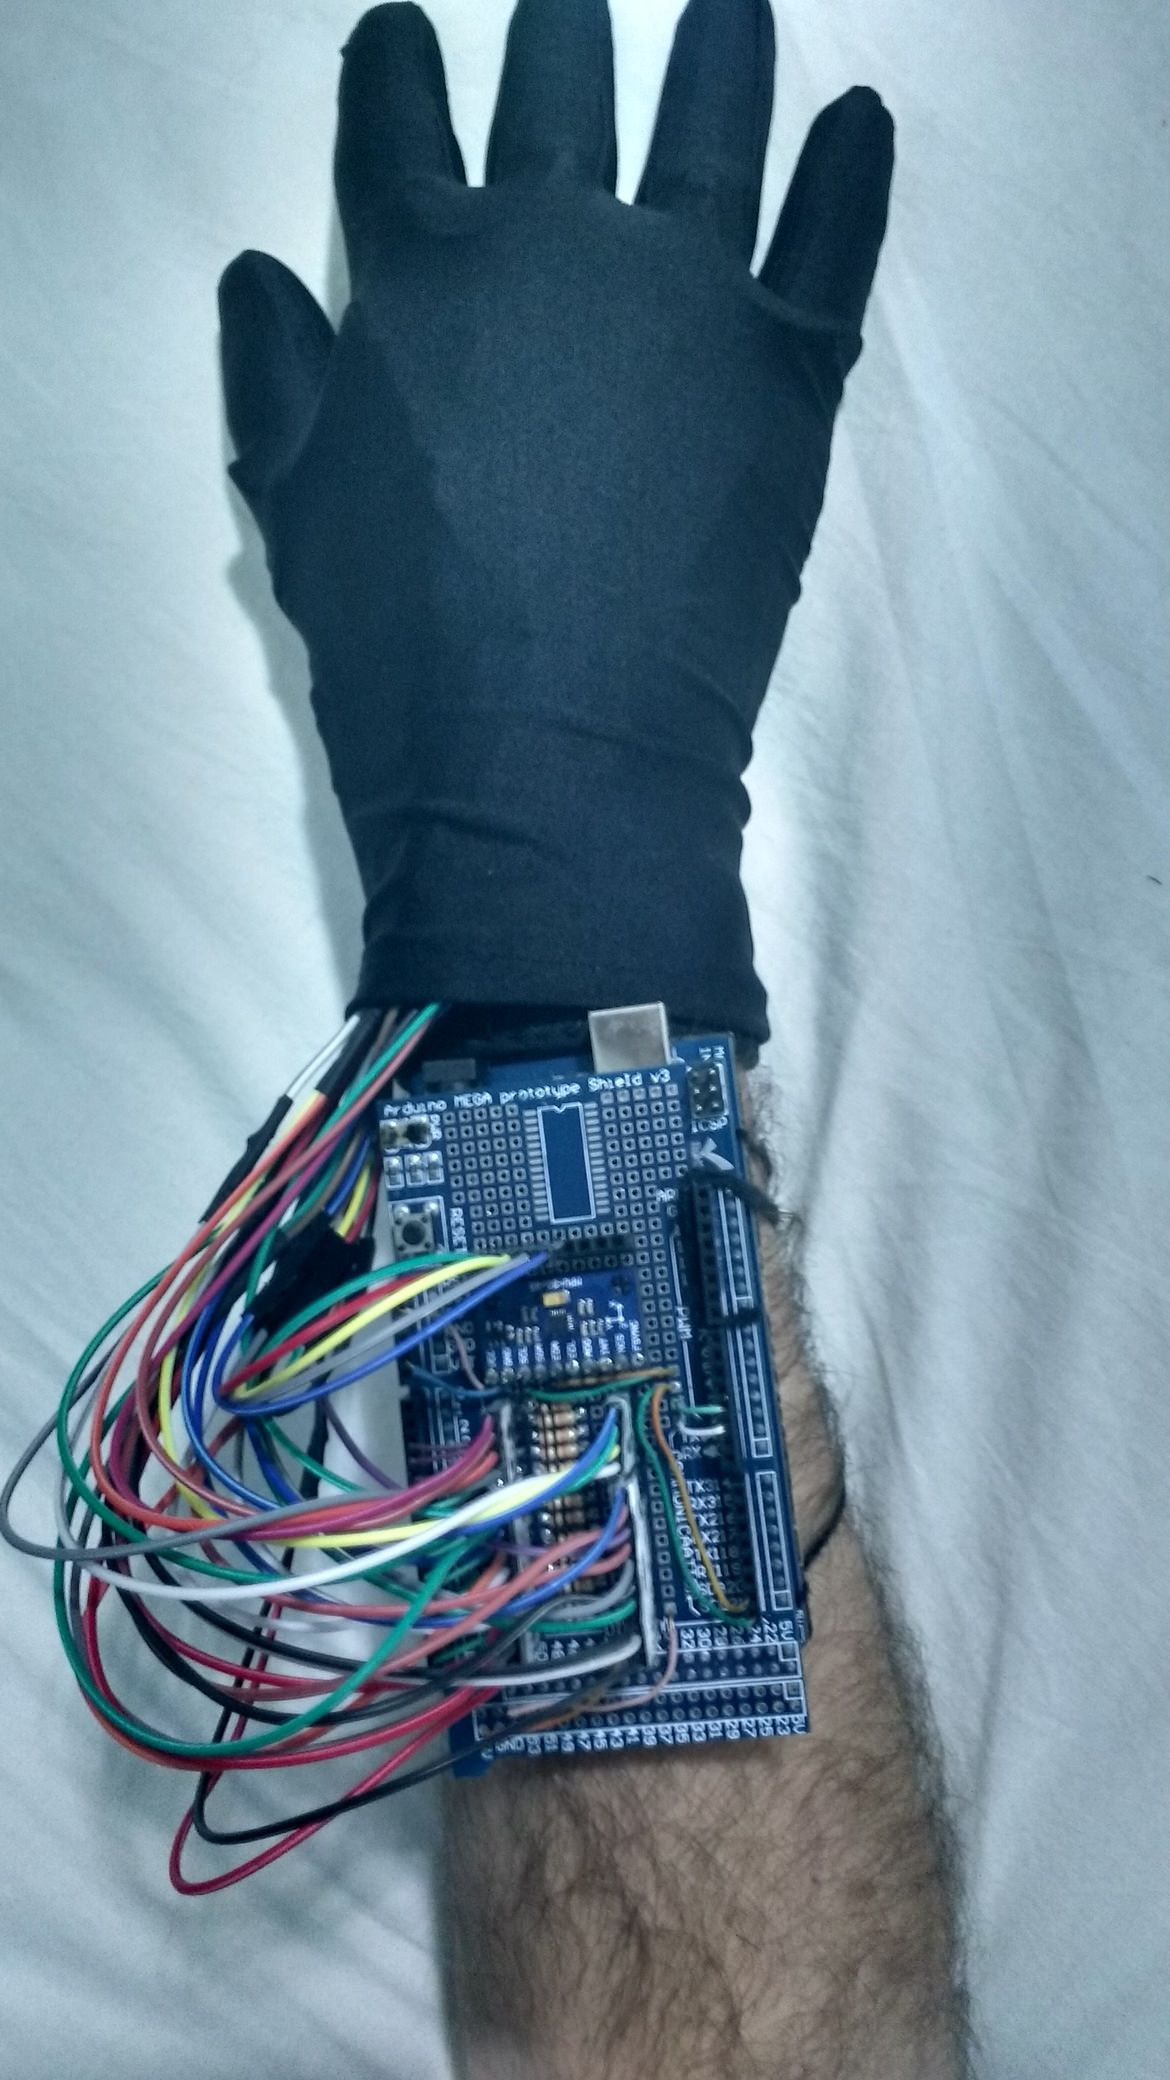
\includegraphics[width=.4\textwidth,angle=90]{imagem/luvanamaocima.jpg}\label{fig:luva_mao_cima}}]
  \\
  \subfloat[Vista lateral]{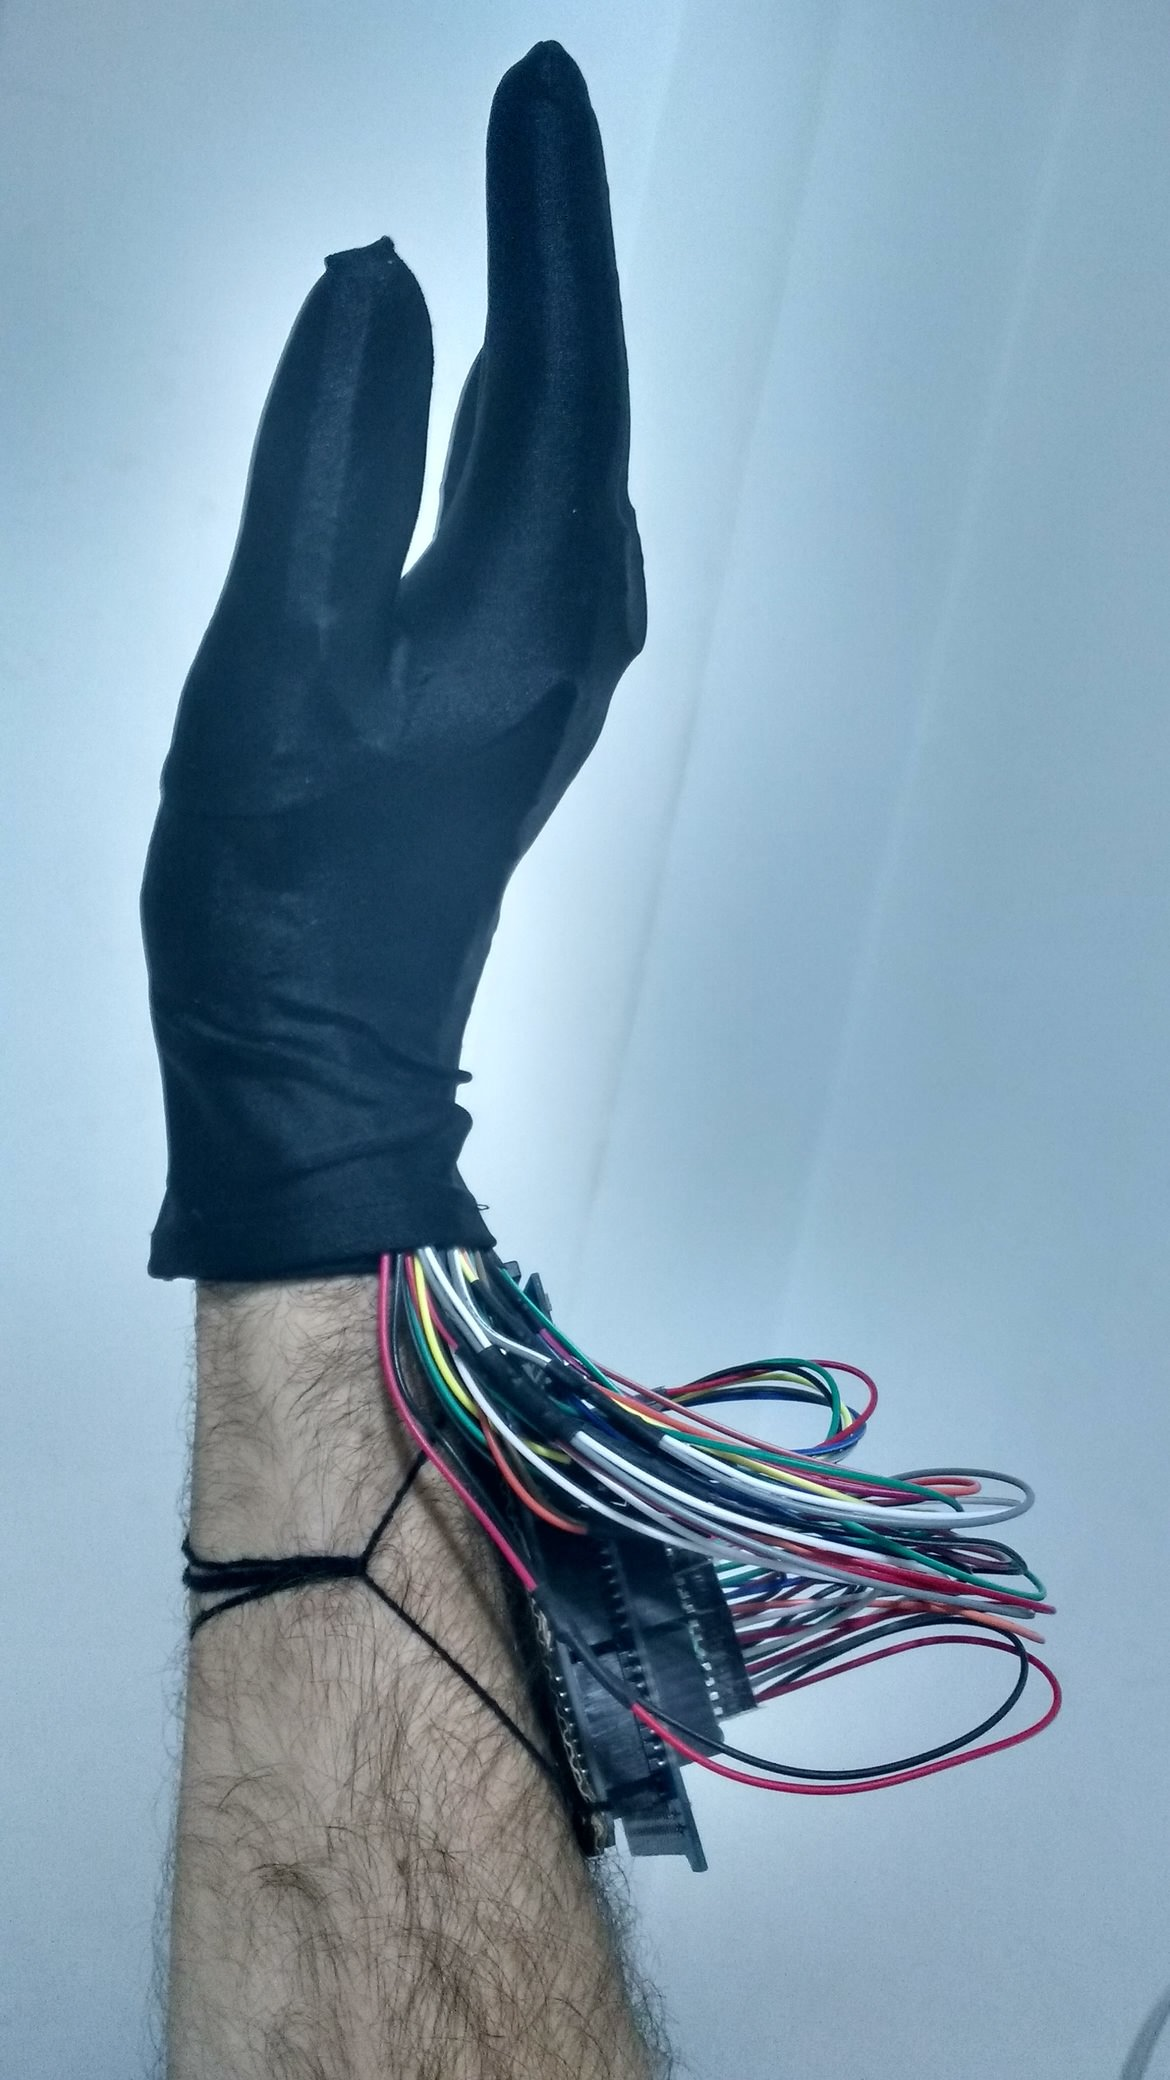
\includegraphics[width=.4\textwidth,angle =90]{imagem/luvanamaolateral.jpg}\label{fig:luva_mao_lateral}}\\
  \captionsetup{justification=centering}
  \captionfont{\small{\textbf{\\Fonte: Elaborado pelo Autor}}}
  \label{fig:luva_mao}
\end{figure}

% subsubsection mpu_9250 (end)

\subsection{Circuito} % (fold)
\label{sub:met_circuito}
O circuito elétrico (Apêndice \ref{apend:circ}) consiste nos 14 sensores de flexão, 14 resistores de \SI{10}{\kilo\ohm} e duas \ac{IMU}s \textit{MPU-9250}. Os 14 resistores e uma das \ac{IMU}s foram soldados em um \textit{shield} de prototipagem, junto com conectores para os sensores de flexão e a segunda \ac{IMU}. O circuito montado é apresentado nas Figuras \ref{fig:placacima} e \ref{fig:placabaixo}, e o circuito modificado de \citeonline{roversi} nas Figuras \ref{fig:placagusbaixo} e \ref{fig:placagusbaixo}.

Os sensores de flexão precisam dos resistores de valor fixo para que seja formado um divisor de tensão, tornando possível medir a queda de tensão no sensor, que é então detectada pelo \textit{Arduino}. Valores entre \SI{10}{\kilo\ohm} e \SI{100}{\kilo\ohm} são comuns para este tipo de sensor \cite{sparkflex} e, como os resistores de \SI{10}{\kilo\ohm} ofereceram resultados aceitáveis, esse valor foi escolhido.

As duas \ac{IMU}s são alimentadas com \SI{3.3}{\volt} e se conectam com o \textit{Arduino} através do protocolo \ac{I2C}, portanto seus pinos \ac{SCL} e \ac{SDA} se conectam aos pinos correspondentes no \textit{Arduino}. Os pinos AD0 são usados para definir o último \textit{bit} do endereço \ac{I2C} de 7 bits \cite{specmpu9250}, possibilitando que sejam conectadas duas \ac{IMU}s com endereços 0x68 (0b1101000), quando AD0 está conectado a \ac{GND} e 0x69 (0b1101001), quando conectado a \SI{3.3}{\volt}. Os pinos \ac{INT} são conectados aos pinos digitais 2 e 3, que são os pinos que podem ser utilizados para interrupções do processador do \textit{Arduino}.

Conectores de barra soldados ao \textit{shield} foram utilizados para que se possa desconectar a luva do \textit{Arduino} para facilitar o manuseio e também para permitir a realização de testes com o protótipo original.

\begin{figure}[ht!]
  \setlength{\abovecaptionskip}{0pt}
  \setlength{\belowcaptionskip}{0pt}
  \caption[Circuito no \textit{shield} de prototipagem]{Circuito no \textit{shield} de prototipagem}
  \centering
  \subfloat[Vista Superior]{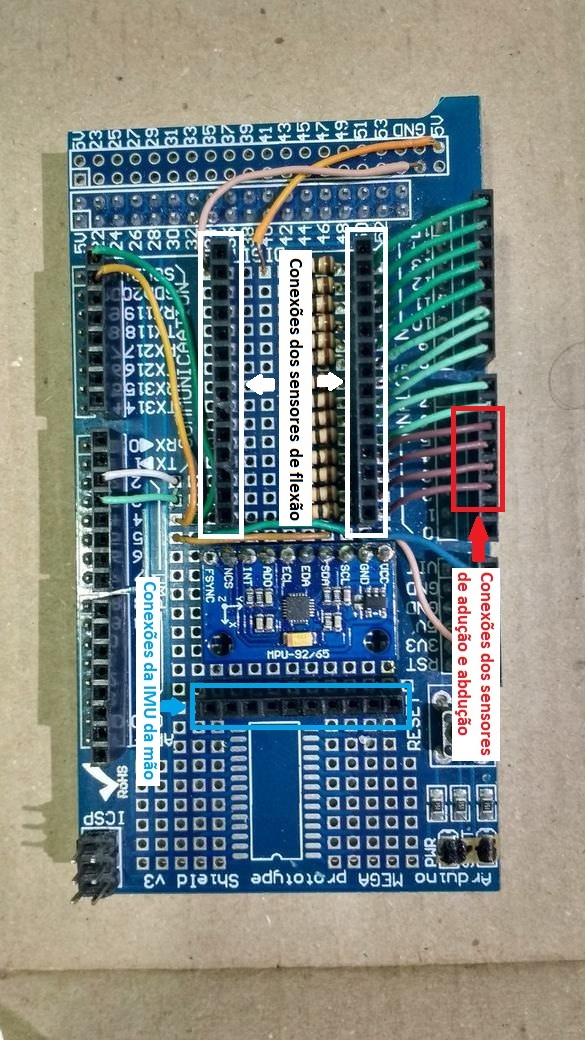
\includegraphics[trim=50 130 60 75,clip,width=.27\textwidth,angle=90]{imagem/placaCima}\label{fig:placacima}}
  \quad
  \subfloat[Vista Inferior]{\includegraphics[trim=130 300 150 200,clip,width=.27\textwidth,angle=90]{imagem/placaBaixo}\label{fig:placabaixo}}\\
  \subfloat[Vista Superior (\citeonline{roversi})]{\includegraphics[width=.27\textwidth,angle=90]{imagem/placaGusCima}\label{fig:placaguscima}}
  \quad
  \subfloat[Vista Inferior (\citeonline{roversi})]{\includegraphics[width=.27\textwidth,angle=90]{imagem/placaGusBaixo}\label{fig:placagusbaixo}}
  \captionsetup{justification=centering}
  \captionfont{\small{\textbf{\\Fonte: Elaborado pelo Autor}}}
  \label{fig:shield}
\end{figure}

No novo circuito foram adicionadas as conexões para os sensores de adução e abdução e conectores de barra para todos os sensores de flexão e para a segunda \ac{IMU} que fica na mão. A \ac{IMU} que fica no \textit{Arduino} também foi rotacionada em relação à de \citeonline{roversi} para que ela tenha a mesma orientção da \ac{IMU} da mão.

% subsubsection circuito (end)
% subsection hardware (end)

\section{Software} % (fold)
\label{sec:met_software}
Nesta etapa foram implementados os códigos do \textit{Arduino} (Apêndice \ref{apend:codigoArd}) e \textit{Unity} (Apêndice \ref{apend:codigoUni}). Na Figura \ref{fig:proc} é mostrado o diagrama de processos, que mostra o funcionamento do sistema como um todo.

O \textit{Arduino} inicializa as duas \ac{IMU}s e seus respectivos \ac{DMP}s. Quando inicializados, os dados dos sensores de flexão são atualizados até que ocorra uma interrupção por parte da \textit{MPU-9250}. Quando isso ocorre, os valores de orientação são atualizados e enviados à \textit{Unity}, se essa requisitou os valores mais atuais.

A \textit{Unity} começa sua execução abrindo uma conexão com a porta serial para recebimento dos dados do \textit{Arduino}. A cada atualização de \textit{frame} é enviado um caractere pela porta serial indicando que a \textit{Unity} precisa dos dados mais recentes para atualizar as posições dos objetos. Após receber e dividir a \textit{string} contendo os dados, a posição de cada objeto é atualizada. 

\begin{figure}[H]
  \setlength{\abovecaptionskip}{0pt}
  \setlength{\belowcaptionskip}{0pt}
  \caption[Diagrama de processos]{Diagrama de processos}
  \centering
  \includegraphics[width=\textwidth]{imagem/processos}
  \captionsetup{justification=centering}
  \captionfont{\small{\textbf{\\Fonte: Elaborado pelo Autor}}}
  \label{fig:proc}
\end{figure}

\subsection{Código do Arduino} % (fold)
\label{sub:codigo_do_arduino}
O código do \textit{Arduino} é responsável por ler os valores dos sensores de flexão e das \ac{IMU}s e enviá-los pela porta serial à \textit{Unity}.

Para a aquisição dos dados das \ac{IMU}s, foi utilizada a biblioteca \textit{I2Cdevlib}, de \citeonline{i2c}, que facilita a comunicação através do protocolo \ac{I2C}, que é o protocolo utilizado pelas \ac{IMU}s, e a biblioteca de \citeonline{9250DMP}, que permite a utilização e configuração do \ac{DMP} do \textit{MPU-9250}.
Para a leitura dos valores dos sensores de flexão foi utilizada a biblioteca \textit{ResponsiveAnalogRead} de \citeonline{analogread}, que reduz os ruídos das entradas analógicas do \textit{Arduino} com redução mínima de responsividade do sinal.

Como foram utilizadas duas \textit{MPU-9250}, foi preciso criar dois objetos do tipo \lstinline!MPU9250! e inicializá-los com seus respectivos endereços do \textit{bus I2C}. Também foram criados objetos do tipo \lstinline!ResponsiveAnalogRead! para cada sensor e flexibilidade passando como parâmetros o pino onde o sensor está conectado e um valor lógico indicando se o modo \textit{sleep} será ligado ou não. Quando ligado, este modo faz com que os valores lidos parem de mudar quando as variações de entrada são muito pequenas, fazendo com que haja uma pequena perda de precisão ao custo de mais responsividade. Optou-se por desligar esse modo para que se possa captar os pequenos movimentos dos dedos. O Código \ref{lst:inicMPU} mostra a inicialização dos objetos necessários.

\begin{lstlisting}[language=C++,label=lst:inicMPU,caption={Inicialização dos objetos},morekeywords={ResponsiveAnalogRead,MPU9250}]
//Inicialização das MPUs
MPU9250 mpu(0x68);
MPU9250 mpu2(0x69);

//Inicialização dos sensores
ResponsiveAnalogRead sensorPolegar1(15, false);
...
ResponsiveAnalogRead sensorAbPolInd(5, false);
ResponsiveAnalogRead sensorAbIndMed(4, false);
ResponsiveAnalogRead sensorAbMedAne(3, false);
ResponsiveAnalogRead sensorAbAneMin(2, false);
\end{lstlisting}

Também foram declaradas as variáveis globais necessárias para monitoramento das \ac{IMU}s, para os cálculos dos ângulos dos sensores e para envio da \textit{string} pela porta serial.

Na função \lstinline!setup()! do \textit{Arduino}, mostrada no Código \ref{lst:setup}, a comunicação serial foi inicializada com \textit{baud rate} de 115200. Em seguida, as \ac{IMU}s e seus \ac{DMP}s são inicializados. Se não hover falhas na inicialização, os \ac{DMP}s são ligados e os pinos de interrupção são habilitados.

\begin{lstlisting}[language=C++,label=lst:setup,caption={Função setup()},morekeywords={ResponsiveAnalogRead,MPU9250,delay,Serial,begin,println,print,attachInterrupt,pinMode}]
void setup() {
  // inicializa comunicação serial
  Serial.begin(115200);

  // inicializa dispositivos
  mpu.initialize();
  delay(100);
  mpu2.initialize();
  pinMode(INTERRUPT_PIN, INPUT);
  pinMode(INTERRUPT_PIN2, INPUT);

  // carregar e configurar o DMP
  devStatus = mpu.dmpInitialize(0x68);
  devStatus2 = mpu2.dmpInitialize(0x69);

  // Testa se inicialização ocorreu sem erros
  if (devStatus == 0 && devStatus2 == 0) {
    // liga o DMP
    mpu.setDMPEnabled(true);
    mpu2.setDMPEnabled(true);

    // Habilita detecção de interrupções do Arduino
    attachInterrupt(digitalPinToInterrupt(INTERRUPT_PIN), dmpDataReady, RISING);
    mpuIntStatus = mpu.getIntStatus();
    attachInterrupt(digitalPinToInterrupt(INTERRUPT_PIN2), dmpDataReady2, RISING);
    mpuIntStatus2 = mpu2.getIntStatus();

    // configura o flag do DMP para o Loop Principal saber se pode utilizá-lo
    dmpReady = true;
    dmpReady2 = true;

    //recebe tamanho esperado do pacote do DMP para comparação
    packetSize = mpu.dmpGetFIFOPacketSize();
    packetSize2 = mpu2.dmpGetFIFOPacketSize();
  } else {
    // ERRO - devStatus != 0
    // 1 = carregamento inicial de memória falhou
    // 2 = autalizações de connfiguração do DMP falharam
    Serial.println(F("Inicialização do DMP falhou!"));
  }
}
\end{lstlisting}

Na função \lstinline!loop()!, caso os \ac{DMP}s não tenham sido inicializados corretamente, o programa entra em \textit{loop} infinito, pois houve algum erro interno das \ac{IMU}s. Caso contrário, os valores dos sensores de flexão são atualizados (com o método \lstinline!ResponsiveAnalogRead.update()!) enquanto não há interrupções e não há \textit{bytes} para serem lidos nas filas \ac{FIFO} das \ac{IMU}s. Os valores dos sensores de flexão variam de 0 a 1024 de acordo com o quanto foram dobrados,portanto, para obter o ângulo da dobra, utilizou-se a função \lstinline!map(int value, int fromLow, int fromHigh, int toLow, int toHigh)!, que analisa o valor de entrada \lstinline!value! e retorna a conversão dos valores do intervalo \lstinline!fromLow! -- \lstinline!fomHigh! para o intervalo \lstinline!toLow! -- \lstinline!toHigh!. Para cada sensor foi obtido o valor médio das leituras com os dedos estendidos e com os dedos flexionados ao máximo para estabelecer os parâmetros \lstinline!fromLow! e \lstinline!fomHigh!, respectivamente. O parâmetro \lstinline!toLow! foi definido como 0, quando os dedos não estão dobrados, e o parâmetro \lstinline!toHigh! foi definido como \ang{90} para a flexão das articulações \ac{MCF}, \ac{IF} e \ac{IFP}, \ang{45} para a abdução da articulação \ac{MCF} do polegar e \ang{15} para a abdução das articulações \ac{MCF} dos outros dedos. Também foi utilizada a função \lstinline!constrain(val, min, max)!, que limita os possíveis valores da variável \lstinline!val! entre os valores \lstinline!min! e \lstinline!max!, para que os eventuais picos de leitura dos sensores não façam com que o modelo \ac{3D} realize movimentos naturalmente impossíveis. O Código \ref{lst:recebe_sensor_flex} mostra a aquisição dos dados dos sensores de flexão.

\begin{lstlisting}[language=C++,label=lst:recebe_sensor_flex,caption={Leitura dos sensores de flexão},morekeywords={ResponsiveAnalogRead,MPU9250,delay,Serial,begin,println,print,attachInterrupt,pinMode}]
// se programação do DMP falhou, não faça nada
if (!dmpReady || !dmpReady2) return;

// espera interrupção do DMP ou pacotes disponíveis
while ((!mpuInterrupt && fifoCount < packetSize) || (!mpuInterrupt2 && fifoCount2 < packetSize2)) {
    //Leitura dos valores dos sensores de flexibilidade
    sensorPolegar1.update();
    ...
    sensorAbPolInd.update();
    sensorAbIndMed.update();
    sensorAbMedAne.update();
    sensorAbAneMin.update();
    
    //conversão dos valores brutos dos sensores para ângulos
    PolegarGraus1   = map(sensorPolegar1.getValue(),   789, 860, 0, 70);
    constrain(PolegarGraus1,0, 70);
    ...
    grausAbPolInd   = map(sensorAbPolInd.getValue(),   784, 875, 0, -30);
    constrain(grausAbPolInd,0, -30);
    grausAbIndMed   = map(sensorAbIndMed.getValue(),   820, 858, 20, 0);
    constrain(grausAbIndMed,0, 20);
    grausAbMedAne   = map(sensorAbMedAne.getValue(),   875, 910, 20, 0);
    constrain(grausAbMedAne,0, 20);
    grausAbAneMin   = map(sensorAbAneMin.getValue(),   828, 890, 35, 0);
    constrain(grausAbAneMin,0, 35);
}

\end{lstlisting}

A Tabela \ref{tab:sens_val} mostra os pinos do \textit{Arduino} onde cada sensor de flexão está conectado, os valores brutos máximo e mínimo (adimensionais) recebidos dos sensores e os ângulos máximo e mínimo (em graus) que os sensores podem ser dobrados quando se utiliza a luva. Esses ângulos foram possíveis de serem obtidos, pois o tecido da luva limita certos movimentos, como a abdução do polegar, não permitindo a abertura máxima que seria possível sem a luva.

\begin{table}[H]
    \centering
    \footnotesize
    \setlength{\abovecaptionskip}{0pt}
    \setlength{\belowcaptionskip}{0pt}
    \caption[Relação dos valores mínimos e máximos dos sensores de flexão]{Relação dos valores mínimos e máximos dos sensores de flexão}
    \label{tab:sens_val}
    \begin{tabular}{l r r r r r}
      \hline\hline
      Sensor & Pino & Mínimo & Máximo & Ângulo Mínimo (\SI{}{\degree}) & Ângulo Máximo (\SI{}{\degree})\\
      \hline
      Polegar (MCF)              & 15 & 789 & 860 & 0 & 70\\
      Polegar (IF)               & 14 & 740 & 851 & 0 & 100\\
      Indicador (MCF)            & 13 & 761 & 884 & 0 & 80\\
      Indicador (IFP)            & 12 & 702 & 753 & 0 & 100\\
      Médio (MCF)                & 11 & 742 & 899 & 0 & 80\\
      Médio (IFP)                & 10 & 747 & 900 & 0 & 100\\
      Anelar (MCF)               & 9  & 740 & 849 & 0 & 80\\
      Anelar (IFP)               & 8  & 713 & 767 & 0 & 100\\
      Mínimo (MCF)               & 7  & 721 & 871 & 0 & 80\\
      Mínimo (IFP)               & 6  & 731 & 827 & 0 & 100\\
      Adução - Polegar/Indicador & 5  & 784 & 875 & 0 & 30\\
      Adução - Indicador/Médio   & 4  & 820 & 858 & 0 & 20\\
      Adução - Médio/Anelar      & 3  & 875 & 910 & 0 & 20\\
      Adução - Anelar/Mínimo     & 2  & 828 & 890 & 0 & 35\\
      \hline \hline
    \end{tabular}
    \\\vspace{1.3mm}
    \captionfont{\small{\textbf{Fontes: Elaborado pelo Autor}}}
\end{table}

Quando ocorrer alguma interrupção, são obtidos os valores filtrados das \ac{IMU}s no formato de Quatérnios, que são representações de orientação no espaço utilizando quatro coordenadas complexas $X$, $Y$, $Z$ e $W$. Esse formato foi escolhido pois fornecia dados mais confiáveis, o que não ocorria ao obter os valores de rotação no formato de Ângulos de Euler (ângulos em torno dos três eixos $X$, $Y$ e $Z$). Ao rotacionar a \textit{MPU-9250} em apenas um eixo, os outros dois sofriam influências quando se obtinha os dados no formato de ângulos de Euler, o que resultava em uma representação incorreta de orientação, mas utilizando quatérnios, o modelo \ac{3D} se comportou corretamente. No Código \ref{lst:recebe_orientacao}, o método \lstinline!MPU9250.dmpGetQuaternion()! obtém os dados das duas \ac{IMU}s.

\begin{lstlisting}[language=C++,label=lst:recebe_orientacao,caption={Leitura das \textit{IMUs}},morekeywords={ResponsiveAnalogRead,MPU9250,delay,Serial,begin,println,print,attachInterrupt,pinMode}]
// recebe os valores de orientação na forma de quatérnios
mpu.dmpGetQuaternion(&q, fifoBuffer);
mpu2.dmpGetQuaternion(&q2, fifoBuffer2);
\end{lstlisting}

Após obter os dados de todos os sensores, o \textit{buffer} de entrada é verificado para saber se a \textit{Unity} requisitou os valores dos ângulos e orientações. Em caso positivo, a \textit{string} era montada com os valores de orientação das duas \ac{IMU}s e os ângulos de dobra dos sensores, estes eram enviados pela porta serial e o processo era repetido. Essa lógica está representada no Código \ref{lst:envia_serial}.

\begin{lstlisting}[language=C++,label=lst:envia_serial,caption={Envio dos dados pela porta serial},morekeywords={ResponsiveAnalogRead,MPU9250,delay,Serial,begin,println,print,attachInterrupt,pinMode}]
if (Serial.available() > 0){
  //consome os bytes do buffer de entrada
  Serial.read();
  
  //Construção da string para ser escrita na porta serial
  valores  = String(PolegarGraus1) + ";"; //ângulo de dobra da MCF do Polegar
  ...
  valores += String(grausAbPolInd) + ";"; //ângulo de dobra entre Polegar e Indicador
  valores += String(grausAbIndMed) + ";"; //ângulo de dobra entre Indicador e Médio
  valores += String(grausAbMedAne) + ";"; //ângulo de dobra entre Médio e Anelar
  valores += String(grausAbAneMin) + ";"; //ângulo de dobra entre Anelar e Mínimo
  
  //orientação do braço
  valores += String(q.w,4) + ";";
  valores += String(q.x,4) + ";";
  valores += String(q.y,4) + ";";
  valores += String(q.z,4) + ";";
  
  //orientação da mão
  valores += String(q2.w,4) + ";";
  valores += String(q2.x,4) + ";";
  valores += String(q2.y,4) + ";";
  valores += String(q2.z,4);
  
  //envia valores  para porta serial
  Serial.println(valores);
}
\end{lstlisting}

% subsubsection código_do_arduino (end)

\subsection{Código da Unity} % (fold)
\label{sub:codigo_da_unity}

Primeiramente, como mostrado no Código \ref{lst:declaracao_unity}, são declaradas as variáveis e objetos necessários para utilização da porta serial e manipulações dos objetos na tela, além de variáveis para receber os dados do \textit{Arduino}. 

\begin{lstlisting}[language=C++,label=lst:declaracao_unity,caption={Declaração de variáveis da \textit{Unity}},morekeywords={SerialPort,IsOpen,Close,Open,Quaternion,GameObject,Vector3,Split,transform,localEulerAngles,Parse,Set,eulerAngles}]
//Declaração de variáveis
SerialPort serial = new SerialPort ("COM4", 115200);
public string ArduinoRead="";
public GameObject firstBone1, firstBone2, firstBone3, firstBone4, firstBone5;
public GameObject middleBone1, middleBone2, middleBone3, middleBone4, middleBone5;
public GameObject lastBone1, lastBone2, lastBone3, lastBone4, lastBone5;
public GameObject hand, arm;
public Vector3 rotacaoMao, rotacaoBraco, rotacaoFinal;
public string[] Output;
float w, x, y, z, w2, x2, y2, z2;
Quaternion quaternionBraco, quaternionMao, quaternionFinal;
\end{lstlisting}

Por padrão, um \textit{script} da \textit{Unity} precisa de duas funções: \lstinline!Start()! e \lstinline!Update()!. A função \lstinline!Start()! é executada uma vez quando a aplicação é aberta e, no caso desse projeto, é usada para abrir a comunicação com a porta serial especificada anteriormente através do método \lstinline!SerialPort.Open()!. A propriedade \lstinline!SerialPort.ReadTimeout! define a quantidade máxima de milissegundos que se deve esperar quando uma operação de leitura não termina. O valor de 100 foi escolhido, pois o envio dos dados pelo \textit{Arduino} não demora mais do que \SI{100}{\milli\second}. A função \lstinline!Start()! é mostrada no Código \ref{lst:unity_start}.

\begin{lstlisting}[language=C++,label=lst:unity_start,caption={Função Start()},morekeywords={SerialPort,IsOpen,Close,Open,Quaternion,GameObject,Vector3,Split,transform,localEulerAngles,Parse,Set,eulerAngles,ReadTimeout}]
//Configuração da conexão da porta
void Start (){
	serial.Open ();
	serial.ReadTimeout = 100;
}
\end{lstlisting}


A função \lstinline!Update()! é chamada a cada atualização de \textit{frame} e é utilizada para manipular os objetos na tela. Essa função verifica se a porta serial ainda está aberta e, em caso positivo, os dados são requisitados ao \textit{Arduino} enviando um caractere pela porta serial. Em seguida, a \textit{string} recebida é lida e armazenada na variável \lstinline!ArduinoRead!, como mostrado no Código \ref{lst:unity_update}.

A \textit{string} é uma série de valores separados por \lstinline!;!, portanto deve ser dividida com o método \lstinline!String.Split(char[] separator)!, onde \lstinline!separator! é o caractere delimitador que separa um elemento do outro na \textit{string}. O vetor resultante com os resultados é armazenado na variável \lstinline!Output!.

\begin{lstlisting}[language=C++,label=lst:unity_update,caption={Função Update()},morekeywords={SerialPort,IsOpen,Close,Open,Quaternion,GameObject,Vector3,Split,transform,localEulerAngles,Parse,Set,eulerAngles}]
void Update (){
	//verifica se a porta serial está aberta
	if (serial.IsOpen) {
		//envia caractere pela porta serial, indicando que estamos prontos para atualizar as posições
		serial.Write("o");
		
		//lê contaúdo da porta serial
		ArduinoRead = serial.ReadLine ();
		
		//separação dos valores da string
		Output = ArduinoRead.Split (new char[] { ';' }, StringSplitOptions.RemoveEmptyEntries);
...
\end{lstlisting}

O próximo passo é movimentar os objetos na tela com a propriedade \lstinline!GameObject.transform.localEulerAngles!, que recebe um vetor \ac{3D} do tipo \lstinline!Vector3(float x, float y, float z)!, onde \lstinline!x!, \lstinline!y! e \lstinline!z! são os ângulos de rotação em torno de cada eixo. A propriedade \lstinline!localEulerAngles! define os ângulos de inclinação de um objeto tomando como referência o seu objeto-pai, ou seja, o objeto ao qual ele está conectado.

O movimento das articulações \ac{MCF} em torno do eixo $Z$ se dá de acordo com os ângulos recebidos dos sensores \ac{MCF} e, o movimento do eixo $Y$ se dá de acordo com os sensores de abdução. Os sensores dos ângulos de abdução apenas detectam os ângulos entre os dedos, o que dificulta o processo de movimentação do modelo\ac{3D}, já que não há uma referência fixa a partir da qual esses ângulos seriam calculados. Para contornar esse problema, considerou-se que o dedo médio não se movimenta durante a abdução ou adução, como mencionado por \citeonline{li2009smartglove}, tornando possível o cálculo dos ângulos de abdução dos dedos indicador, anelar tendo o dedo médio como referência, e o ângulo de abdução do dedo mínimo sendo definido pela Equação \ref{eq:minimo}, onde $\theta_{\text{Médio/Anelar}}$ é a abdução entre os dedos médio e anelar, e $\theta_{\text{Anelar/Mínimo}}$ é a abdução entre os dedos anelar e mínimo. A adução do polegar já possui como referência fixa a articulação \ac{MCF} do dedo indicador.

\begin{equation}\label{eq:minimo}
    \theta_{\text{Mínimo}} = \theta_{\text{Médio/Anelar}}+\theta_{\text{Anelar/Mínimo}}
\end{equation}


Para a articulação \ac{MCF} do polegar, as rotações sobre os eixos $Y$ e $Z$ foram fixadas para compensar a posição do objeto no modelo da \textit{Unity}, já que o polegar está a um ângulo diferente dos outros dedos. As articulações \ac{IF} do polegar e \ac{IFP} dos demais dedos se movimentam apenas em torno do eixo $Z$, portanto apenas essa componente foi modificada, como mostra o Código \ref{lst:dedos_transform}. Para as articulações \ac{IFD} foi feito o cálculo mencionado em \citeonline{li2009smartglove}, onde o ângulo de dobra dessa articulação tem relação com a articulação \ac{IFP} de acordo com a Equação \ref{eq:ifd}.

\begin{equation}\label{eq:ifd}
    \theta_{IFD} = \frac{2}{3} \theta_{IFP}
\end{equation}

\begin{lstlisting}[language=C++,label=lst:dedos_transform,caption={Transformações dos dedos},morekeywords={SerialPort,IsOpen,Close,Open,Quaternion,GameObject,Vector3,Split,transform,localEulerAngles,Parse,Set,eulerAngles}]
//atualização das posições dos dedos
//Polegar
firstBone1.transform.localEulerAngles = new Vector3 (int.Parse (Output [10])-50, 225, 90);
middleBone1.transform.localEulerAngles = new Vector3 (0, 0, int.Parse (Output [0]));
lastBone1.transform.localEulerAngles = new Vector3 (0, 0, int.Parse (Output [1]));
//Indicador
firstBone2.transform.localEulerAngles = new Vector3 (0, -int.Parse (Output [11]), int.Parse (Output [2]));
middleBone2.transform.localEulerAngles = new Vector3 (0, 0, int.Parse (Output [3]));
lastBone2.transform.localEulerAngles = new Vector3 (0, 0, int.Parse (Output [3]) * 2 / 3);
//Médio
firstBone3.transform.localEulerAngles = new Vector3 (0, 0, int.Parse (Output [4]));
middleBone3.transform.localEulerAngles = new Vector3 (0, 0, int.Parse (Output [5]));
lastBone3.transform.localEulerAngles = new Vector3 (0, 0, int.Parse (Output [5]) * 2 / 3);
//Anelar
firstBone4.transform.localEulerAngles = new Vector3 (0, int.Parse (Output [12]), int.Parse (Output [6]));
middleBone4.transform.localEulerAngles = new Vector3 (0, 0, int.Parse (Output [7]));
lastBone4.transform.localEulerAngles = new Vector3 (0, 0, int.Parse (Output [7]) * 2 / 3);
//Mínino
firstBone5.transform.localEulerAngles = new Vector3 (0, int.Parse (Output [13])+int.Parse (Output [12])-10, int.Parse (Output [8]));
middleBone5.transform.localEulerAngles = new Vector3 (0, 0, int.Parse (Output [9]));
lastBone5.transform.localEulerAngles = new Vector3 (0, 0, int.Parse (Output [9]) * 2 / 3);
\end{lstlisting}

Finalmente foi realizada a transformação da mão em relação ao braço, criando os objetos do tipo \lstinline!Quaternion! e os inicializando com os valores dos quatérnios recebidos do \textit{Arduino}, como mostra o Código \ref{lst:mao_transform}. Os quatérnios são então convertidos em ângulos de Euler e é realizada a subtração dos ângulos de rotação entre a mão e o braço, a fim de obter a orientação da mão em relação ao braço, o que resulta nos movimentos de extensão, flexão e desvios radial e ulnar do pulso.

\begin{lstlisting}[language=C++,label=lst:mao_transform,caption={Transformações da mão},morekeywords={SerialPort,IsOpen,Close,Open,Quaternion,GameObject,Vector3,Split,transform,localEulerAngles,Parse,Set,eulerAngles}]
//variáveis dos quatérnios da mão e do braço
w = float.Parse (Output [14]);
x = float.Parse (Output [15]);
y = float.Parse (Output [16]);
z = float.Parse (Output [17]);
w2 = float.Parse (Output [18]);
x2 = float.Parse (Output [19]);
y2 = float.Parse (Output [20]);
z2 = float.Parse (Output [21]);

//atribuição dos objetos dos quatérnios de acordo com as variáveis anteriores
quaternionBraco.Set (x, -z, y, w);
quaternionMao.Set (x2, -z2, y2, w2);

//cálculo da diferença entre os ângulos de orientação
rotacaoFinal = quaternionMao.eulerAngles-quaternionBraco.eulerAngles;

//permite rotação do braço apenas em torno do eixo X
quaternionBraco.Set (x, 0, 0, w);

//Atualiza as rotações do braço e da mão
arm.transform.rotation = quaternionBraco;
hand.transform.localEulerAngles = rotacaoFinal;
\end{lstlisting}
% subsection código_da_unity (end)

% subsection software (end)
% Nome do capítulo
\chapter{Resultados}
% Label para referenciar
\label{ch:resultados}

% Diminuir espaçamento entre título e texto
\vspace{-1.9cm}

Neste capítulo serão discutidos os resultados obtidos durante os testes, realizadas comparações e destacadas melhorias em relação à luva desenvolvida por \citeonline{roversi}.

\section{Comparação com protótipo de \citeonline{roversi}}
\label{sec:comp}

Com relação à luva de \citeonline{roversi} foi percebido que o material utilizado possibilitou uma melhor fixação dos sensores, porém foi difícil a colocação e remoção da luva por pessoas com mãos grandes (com circunferência da palma da mão com mais de \SI{22}{\centi\metre}). Também percebeu-se que os sensores ficaram melhor fixados quando se colocou a luva de \textit{lycra} por cima, já que esta auxilia que os sensores se curvem com os dedos quando dobrados ao máximo.

A comparação com a luva de \citeonline{roversi} foi feita posicionando a luva em cada uma das posições apresentadas na Figura \ref{fig:pos} e analisando as leituras dos sensores de flexão e das \ac{IMU}s. Cada posição foi mantida por 10 segundos e foram calculados média, \ac{DP}, amplitude e \ac{DMA} para cada sensor.

O filtro aplicado sobre os sensores de flexão foi parcialmente satisfatório, promovendo boa redução de ruído sem comprometer a responsividade dos movimentos, mas não oferecendo boa resolução de detecção. Em certas ocasiões os sensores produziam muitos ruídos que, mesmo após a aplicação do filtro, causavam movimentos súbitos no modelo \ac{3D}. A seguir serão apresentadas as comparações dos resultados obtidos usando o circuito e o código de \citeonline{roversi}, e usando o circuito e o código deste trabalho.

A Tabela \ref{tab:an_est_plan} mostra a análise dos ângulos obtidos de cada sensor de flexão com os dedos na posição 1, apresentada na Seção \ref{sub:testes}. A média, \ac{DP}, Amplitude e \ac{DMA} são dados em graus e os ângulos reais considerados para os cálculos foram de \ang{0} para todos os dedos. Pode-se perceber uma redução do \ac{DP} e amplitude em relação ao trabalho de \citeonline{roversi}, indicando que os filtros para redução do ruído dos sensores contribuíram para suavizar os movimentos realizados. Percebe-se também que o \ac{DMA} de alguns sensores foi muito alto, chegando a um desvio de até \ang{18}. Isso ocorreu devido às interferências entre um sensor e outro, causando leituras incorretas em certas posições.

\begin{table}[H]
  \centering
  \footnotesize
  \setlength{\abovecaptionskip}{0pt}
  \setlength{\belowcaptionskip}{0pt}
  \caption[Análise das leituras sensores de flexão na posição plana]{Análise das leituras sensores de flexão na posição plana}
  \label{tab:an_est_plan}
\begin{tabular}{l|rrrr|rrrr}
    \hline\hline
	\multirow{2}{*}{Sensor} & \multicolumn{4}{c|}{Este Trabalho} & \multicolumn{4}{c}{\citeonline{roversi}} \\
	\cline{2-9}
    \multirow{1}{*}{} & \multicolumn{1}{c}{Média}       & \multicolumn{1}{c}{\ac{DP}} & \multicolumn{1}{c}{Amplitude} & \multicolumn{1}{c|}{\ac{DMA}} & \multicolumn{1}{c}{Média}       & \multicolumn{1}{c}{\ac{DP}} & \multicolumn{1}{c}{Amplitude} & \multicolumn{1}{c}{\ac{DMA}} \\
    \hline
    Pol. MCF  & 5,119 & 1,036 & 8,000 & 5,119 & 9,043 & 1,618 & 18,000 & 9,043 \\
    Pol. IF  & 12,995 & 3,225 & 9,000 & 12,995 & 6,138 & 0,768 & 9,000 & 6,138 \\
    Ind. MCF  & 0,014 & 0,117 & 1,000 & 0,014 & 0,021 & 0,292 & 4,000 & 0,053 \\
    Ind. IFP  & 9,064 & 0,353 & 2,000 & 9,064 & 1,681 & 1,698 & 13,000 & 1,894 \\
    Med. MCF  & 0,000 & 0,000 & 0,000 & 0,000 & -0,059 & 0,257 & 2,000 & 0,059 \\
    Med. IFP  & 9,367 & 0,776 & 2,000 & 9,367 & 2,426 & 0,774 & 5,000 & 2,426 \\
    Ane. MCF  & -5,005 & 0,068 & 1,000 & 5,005 & 7,218 & 1,019 & 10,000 & 7,218 \\
    Ane. IFP  & -0,028 & 0,345 & 5,000 & 0,028 & -2,824 & 1,858 & 19,000 & 2,973 \\
    Min. MCF  & 1,000 & 0,000 & 0,000 & 1,000 & 0,638 & 0,722 & 5,000 & 0,638 \\
    Min. IFP  & 9,005 & 0,068 & 1,000 & 9,005 & -0,101 & 0,850 & 6,000 & 0,420 \\
    Pol./Ind. & -39,005 & 0,068 & 1,000 & 9,005 & -- & -- & -- & -- \\
    Ind./Med. & -1,000 & 0,000 & 0,000 & 1,000 & -- & -- & -- & -- \\
    Med./Ane. & -1,005 & 0,068 & 1,000 & 1,005 & -- & -- & -- & -- \\
    Ane./Min. & 18,995 & 0,068 & 1,000 & 18,995 & -- & -- & -- & -- \\
    \hline\hline
\end{tabular}
  \\\vspace{1.3mm}
  \captionfont{\small{\textbf{Fonte: Elaborado pelo Autor}}}
\end{table}

O Gráfico \ref{fig:graf_sensflex} a seguir apresenta os dados dos sensores de flexão das articulações \ac{MCF} e \ac{IF} do polegar obtidos por \citeonline{roversi} (Gráfico \ref{fig:sensflexgus}) e por este trabalho (Gráfico \ref{fig:sensflexmeu}). Nota-se que filtro aplicado eliminou boa parte dos ruídos existentes.    

\begin{grafico}[H]
  \setlength{\abovecaptionskip}{0pt}
  \setlength{\belowcaptionskip}{0pt}
  \caption[Leituras dos sensores de flexão do polegar]{Leituras dos sensores de flexão do polegar}
  \centering
  \subfloat[Leituras obtidas com circuito e código de \citeonline{roversi}]{\includegraphics[width=.8\textwidth]{imagem/sensflex_pol1-2_bruto_gustavo}\label{fig:sensflexgus}}\\
  %\subfloat[Leituras obtidas com o circuito e código deste  trabalho]{\includegraphics[width=.6\textwidth]{imagem/sensflex_pol1-2_filtrado_bruto_meu}\label{fig:sensflexmeu}}
  \captionsetup{justification=centering}
  \captionfont{\small{\textbf{\\Fonte: Elaborado pelo Autor}}}
  \label{fig:graf_sensflex}
\end{grafico}

\begin{grafico}[H]
    \ContinuedFloat
  \setlength{\abovecaptionskip}{0pt}
  \setlength{\belowcaptionskip}{0pt}
  \caption[Leituras dos sensores de flexão do polegar (Cont.)]{Leituras dos sensores de flexão do polegar (Cont.)}
  \centering
  %\subfloat[Leituras obtidas com circuito e código de \citeonline{roversi}]{\includegraphics[width=.6\textwidth]{imagem/sensflex_pol1-2_bruto_gustavo}\label{fig:sensflexgus}}\\
  \subfloat[Leituras obtidas com o circuito e código deste  trabalho]{\includegraphics[width=.85\textwidth]{imagem/sensflex_pol1-2_filtrado_bruto_meu}\label{fig:sensflexmeu}}
  \captionsetup{justification=centering}
  \captionfont{\small{\textbf{\\Fonte: Elaborado pelo Autor}}}
  \label{fig:graf_sensflex2}
\end{grafico}

O \textit{MPU-6050} utilizado por \citeonline{roversi} gerava muitos ruídos pois utilizava somente as leituras do acelerômetro. Isso foi solucionado utilizando o \textit{MPU-9250} e utilizando o seu processador interno, o \ac{DMP}, para realizar a fusão dos dados do acelerômetro, giroscópio e magnetômetro embutidos, o que produziu um sinal quase completamente livre de ruídos e bastante responsivo. Os Gráficos \ref{fig:grafmpu9250} e \ref{fig:grafmpu6050} foram gerados com a \textit{MPU-9250} e \textit{MPU-6050} em uma superfície plana. Pode-se perceber que as leituras da \textit{MPU-9250} com o \ac{DMP} são quase completamente livres de ruídos, enquanto que as leituras da \textit{MPU-6050} sem o \ac{DMP} são mais instáveis. Ainda se observou o efeito de \textit{drift} durante os primeiros 15 segundos de utilização da luva, enquanto as \ac{IMU}s se calibravam, mas após esse período as leituras se estabilizaram, como mostra o Gráfico \ref{fig:grafdrift}.

\begin{grafico}[H]
  \setlength{\abovecaptionskip}{0pt}
  \setlength{\belowcaptionskip}{0pt}
  \caption[Leituras das \ac{IMU}s]{Leituras das \ac{IMU}s}
  \centering
  \subfloat[Leituras da \textit{MPU-6050} sem \ac{DMP}]{\includegraphics[trim=0 0 0 28 ,clip,width=.7\textwidth]{imagem/6050nodmp_plano.png}\label{fig:grafmpu6050}}\\
  %\subfloat[Leituras da \textit{MPU-9250} com \ac{DMP}]{\includegraphics[trim=0 0 0 30 ,clip,width=.7\textwidth]{imagem/9250dmp_plano.png}\label{fig:grafmpu9250}}
  \captionsetup{justification=centering}
  \captionfont{\small{\textbf{\\Fonte: Elaborado pelo Autor}}}
  \label{fig:graf_mpu}
\end{grafico}

\begin{grafico}[H]
\ContinuedFloat
  \setlength{\abovecaptionskip}{0pt}
  \setlength{\belowcaptionskip}{0pt}
  \caption[Leituras das \ac{IMU}s]{Leituras das \ac{IMU}s}
  \centering
  %\subfloat[Leituras da \textit{MPU-6050} sem \ac{DMP}]{\includegraphics[trim=0 0 0 28 ,clip,width=.7\textwidth]{imagem/6050nodmp_plano.png}\label{fig:grafmpu6050}}\\
  \subfloat[Leituras da \textit{MPU-9250} com \ac{DMP}]{\includegraphics[trim=0 0 0 30 ,clip,width=.7\textwidth]{imagem/9250dmp_plano.png}\label{fig:grafmpu9250}}
  \captionsetup{justification=centering}
  \captionfont{\small{\textbf{\\Fonte: Elaborado pelo Autor}}}
  \label{fig:graf_mpu2}
\end{grafico}

\begin{grafico}[H]
  \setlength{\abovecaptionskip}{0pt}
  \setlength{\belowcaptionskip}{0pt}
  \caption[Efeito \textit{drift} da \textit{MPU-9250}]{Efeito \textit{drift} da \textit{MPU-9250}}
  \centering
  \includegraphics[width=.7\textwidth]{imagem/drift_mpu1.png}
  \captionsetup{justification=centering}
  \captionfont{\small{\textbf{\\Fonte: Elaborado pelo Autor}}}
  \label{fig:grafdrift}
\end{grafico}

A Tabela \ref{tab:imu_est_plan} mostra a análise dos ângulos obtidos pelas \ac{IMU}s com a mão e o braço na posição plana. Os cálculos para as \ac{IMU}s deste trabalho foram feitos utilizando a diferença entre os ângulos obtidos das \textit{MPU-9250} do braço e da mão e, os cálculos para a \ac{IMU} de \citeonline{roversi} foram feitos com as devidas conversões dos dados da \textit{MPU-6050}. Nota-se uma redução do \ac{DP}, o que sugere que o \ac{DMP} da \textit{MPU-9250} foi suficiente para redução de ruídos e suavização dos movimentos. Percebe-se também que o \ac{DMA} atingiu uma diferença de até \ang{15}, o que foi causado devido ao mau posicionamento do \textit{Arduino} no braço, pois o mesmo tendia a ficar inclinado em relação à \ac{IMU} da mão.

\begin{table}[H]
  \centering
  \footnotesize
  \setlength{\abovecaptionskip}{0pt}
  \setlength{\belowcaptionskip}{0pt}
  \caption[Análise das leituras das \ac{IMU}s na posição plana]{Análise das leituras das \ac{IMU}s na posição plana}
  \label{tab:imu_est_plan}
\begin{tabular}{l|rrrr|rrrr}
    \hline\hline
	\multirow{2}{*}{Sensor} & \multicolumn{4}{c|}{Este Trabalho - \textit{MPU-9250}} & \multicolumn{4}{c}{\citeonline{roversi} - \textit{MPU-6050}} \\
	\cline{2-9}
    \multirow{1}{*}{} & \multicolumn{1}{c}{Média} & \multicolumn{1}{c}{\ac{DP}} & \multicolumn{1}{c}{Amplitude} & \multicolumn{1}{c|}{\ac{DMA}} & 
    \multicolumn{1}{c}{Média} & 
    \multicolumn{1}{c}{\ac{DP}} & \multicolumn{1}{c}{Amplitude} & \multicolumn{1}{c}{\ac{DMA}} \\
    \hline
IMU - eixo X & -15,276 & 0,680 & 2,280 & 15,165 & 9,263 & 1,630 & 1,500 & 9,263 \\
IMU - eixo Y & -8,108 & 0,466 & 2,110 & 8,005 & 2,398 & 3,051 & 5,000 & 2,398 \\
IMU - eixo Z & 18,167 & 0,707 & 2,160 & 8,332 & 21,327 & 1,220 & 1,500 & 21,327 \\
    \hline\hline
\end{tabular}
  \\\vspace{1.3mm}
  \captionfont{\small{\textbf{Fonte: Elaborado pelo Autor}}}
\end{table}

A Tabela \ref{tab:an_est_ger} mostra as médias do \ac{DP}, Amplitude e \ac{DMA} dos sensores para cada repetição de cada movimento. As posições 1, 2, 3, 4 e 9 foram calculadas com os dados dos sensores de flexão e as posições 5, 6, 7 e 8 forma calculadas com os dados das \ac{IMU}s. Percebe-se que as leituras possuíram \ac{DP} e amplitude menores, indicando que o filtro aplicado reduziu as oscilações indesejadas do modelo. Além disso, a luva deste trabalho possui um \ac{DMA} menor, indicando que os movimentos realizados foram mais precisos que as de \citeonline{roversi}, pois os ângulos calculados forma mais próximos dos ângulos reais.
\begin{table}[H]
  \centering
  \footnotesize
  \setlength{\abovecaptionskip}{0pt}
  \setlength{\belowcaptionskip}{0pt}
  \caption[Análise geral das leituras dos sensores para cada movimento]{Análise geral das leituras dos sensores para cada movimento}
  \label{tab:an_est_ger}
\begin{tabular}{l|rrr|rrr}
\hline\hline
\multirow{2}{*}{Posições} & \multicolumn{3}{c|}{Este Trabalho} & \multicolumn{3}{c}{\citeonline{roversi}} \\
\cline{2-7}
\multirow{1}{*}{} & \multicolumn{1}{c}{\ac{DP}} & \multicolumn{1}{c}{Amplitude} & \multicolumn{1}{c|}{\ac{DMA}} & \multicolumn{1}{c}{\ac{DP}} & \multicolumn{1}{c}{Amplitude} & \multicolumn{1}{c}{\ac{DMA}} \\
\hline			
1 (Mão plana)                  & 0,442  & 2,286  & 5,829  & 0,812  & 7,500  & 2,160 \\
2 (Flexão MCF e IF do polegar) & 0,069  & 0,333  & 7,000  & 2,534  & 15,500 & 10,337 \\
3 (Flexão MCF dos dedos)       & 0,848  & 4,167  & 9,038  & 3,366  & 18,667 & 17,403 \\
4 (Flexão IFP dos dedos)       & 0,301  & 0,667  & 9,209  & 3,551  & 16,000 & 18,840 \\
5 (Extensão do pulso)          & 0,428  & 2,560  & 5,014  & 0,890  & 4,833  & 27,509 \\
6 (Flexão do pulso)            & 0,635  & 2,980  & 4,608  & 0,892  & 4,500  & 5,046 \\
7 (Desvio Ulnar)               & 0,360  & 1,333  & 7,374  & --     & --     & -- \\
8 (Desvio Radial)              & 0,111  & 0,547  & 7,836  & --     & --     & -- \\
9 (Abdução dos dedos)          & 0,239  & 1,180  & 1,800  & --     & --     & -- \\
\hline
Média                          & 0,382  & 1,784  & 6,412  & 2,008  & 11,167 & 13,549 \\
\hline\hline
\end{tabular}
  \\\vspace{1.3mm}
  \captionfont{\small{\textbf{Fonte: Elaborado pelo Autor}}}
\end{table}


O método de comunicação do \textit{Arduino} com a \textit{Unity} no trabalho de \citeonline{roversi} fazia com que muitos dados ficassem presos no \textit{buffer} de entrada da porta serial do computador devido à velocidade de envio. A solução desse trabalho foi que a \textit{Unity} requisitasse os dados ao \textit{Arduino} a cada atualização de \textit{frame}.  Apesar de haver um pequeno atraso em relação ao movimento real e o movimento do modelo, essa solução se mostrou satisfatória, gerando movimentos mais fluidos, já que o modelo \ac{3D} sempre era atualizado com os dados mais recentes.

A Figura \ref{fig:pos_res} a seguir mostra a comparação dos movimentos reais e dos reproduzidos pelo modelo \ac{3D}. É possível notar nas Figuras \ref{fig:pos_3_modelo} e \ref{fig:pos_7_modelo} que a articulação \ac{IFP} do dedo indicador está ligeiramente flexionada devido a ruídos provenientes do sensor de flexão. 

\begin{figure}[H]
  \setlength{\abovecaptionskip}{0pt}
  \setlength{\belowcaptionskip}{0pt}
  \caption[Posições reais seus resultados reproduzidos pelo modelo \ac{3D}]{Posições reais seus resultados reproduzidos pelo modelo \ac{3D}}
  \centering
  \subfloat[Posição 1 - Real]{\includegraphics[width=.4\textwidth]{imagem/p1_real}\label{fig:pos_1_real}}
  \quad
  \subfloat[Posição 1 - Modelo]{\includegraphics[width=.4\textwidth]{imagem/p1}\label{fig:pos_1_modelo}}\\
  \subfloat[Posição 2 - Real]{\includegraphics[width=.4\textwidth]{imagem/p2_real}\label{fig:pos_2_real}}
  \quad
  \subfloat[Posição 2 - Modelo]{\includegraphics[width=.4\textwidth]{imagem/p2}\label{fig:pos_2_modelo}}\\
  \subfloat[Posição 3 - Real]{\includegraphics[width=.4\textwidth]{imagem/p3_real}\label{fig:pos_3_real}}
  \quad
  \subfloat[Posição 3 - Modelo]{\includegraphics[width=.4\textwidth]{imagem/p3}\label{fig:pos_3_modelo}}\\
  \subfloat[Posição 4 - Real]{\includegraphics[width=.4\textwidth]{imagem/p4_real}\label{fig:pos_4_real}}
  \quad
  \subfloat[Posição 4 - Modelo]{\includegraphics[width=.4\textwidth]{imagem/p4}\label{fig:pos_4_modelo}}\\
  \captionsetup{justification=centering}
  \captionfont{\small{\textbf{\\Fonte: Elaborado pelo Autor}}}
  \label{fig:pos_res}
\end{figure}

\begin{figure}[H]
  \ContinuedFloat
  \setlength{\abovecaptionskip}{0pt}
  \setlength{\belowcaptionskip}{0pt}
  \caption[Posições reais seus resultados reproduzidos pelo modelo \ac{3D}]{Posições reais seus resultados reproduzidos pelo modelo \ac{3D}}
  \centering
  \subfloat[Posição 5 - Real]{\includegraphics[width=.4\textwidth]{imagem/p5_real}\label{fig:pos_5_real}}
  \quad
  \subfloat[Posição 5 - Modelo]{\includegraphics[width=.4\textwidth]{imagem/p5}\label{fig:pos_5_modelo}}\\
  \subfloat[Posição 6 - Real]{\includegraphics[width=.4\textwidth]{imagem/p6_real}\label{fig:pos_6_real}}
  \quad
  \subfloat[Posição 6 - Modelo]{\includegraphics[width=.4\textwidth]{imagem/p6}\label{fig:pos_6_modelo}}\\
  \subfloat[Posição 7 - Real]{\includegraphics[width=.4\textwidth]{imagem/p7_real}\label{fig:pos_7_real}}
  \quad
  \subfloat[Posição 7 - Modelo]{\includegraphics[width=.4\textwidth]{imagem/p7}\label{fig:pos_7_modelo}}\\
  \subfloat[Posição 8 - Real]{\includegraphics[width=.4\textwidth]{imagem/p8_real}\label{fig:pos_8_real}}
  \quad
  \subfloat[Posição 8 - Modelo]{\includegraphics[width=.4\textwidth]{imagem/p8}\label{fig:pos_8_modelo}}\\
  \subfloat[Posição 9 - Real]{\includegraphics[width=.4\textwidth]{imagem/p9_real}\label{fig:pos_9_real}}
  \quad
  \subfloat[Posição 9 - Modelo]{\includegraphics[width=.4\textwidth]{imagem/p9}\label{fig:pos_9_modelo}}\\
  \captionsetup{justification=centering}
  \captionfont{\small{\textbf{\\Fonte: Elaborado pelo Autor}}}
  \label{fig:pos_res2}
\end{figure}

\section{Problemas encontrados}
\label{sec:prob}

Após a montagem da luva, o sensor da articulação \ac{IFP} do anelar apresentou ruídos excessivos, mesmo após a aplicação do filtro. As possíveis causas são o mau funcionamento do sensor, ou curto-circuitos causados pela interação com os outros sensores próximos a ele.

Foi observado que valores usados na conversão para o ângulo de dobra dos sensores de flexão podem variar quando o circuito é alterado, ou até mesmo após a recolocação da luva. Essa alteração ocorre devido às variações na posição do tecido da luva, fazendo com que os sensores não fiquem na mesma posição.

Os sensores usados na detecção dos movimentos de adução e abdução eram influenciados pelos movimentos de flexão dos dedos, devido à sua posição na luva (Figura \ref{fig:pos_indic}). Ao estender apenas o dedo indicador, o sensor entre os dedos indicador e médio era deformado, gerando leituras que causavam a abdução desse dedo no modelo \ac{3D}. Para solucionar esse problema deveriam ser criadas regras para ignorar leituras dos sensores de abdução quando apenas um dos dedos se movimentasse.

O tecido da luva e o posicionamento do \textit{Arduino} limitaram certos movimentos como o movimento de abdução do polegar e o de extensão do pulso, que foi interferido pelo cabo \ac{USB}.

\begin{figure}[H]
  \setlength{\abovecaptionskip}{0pt}
  \setlength{\belowcaptionskip}{0pt}
  \caption[Movimentação errada ao estender apenas o dedo indicador]{Movimentação errada ao estender apenas o dedo indicador}
  \centering
  \subfloat[Extensão - Real]{\includegraphics[width=.4\textwidth]{imagem/indicadorabducao_real}\label{fig:indicadorabducao_real}}
  \quad
  \subfloat[Extensão e abdução - Modelo]{\includegraphics[width=.4\textwidth]{imagem/indicadorabducao}\label{fig:indicadorabducao_modelo}}\\
  \captionsetup{justification=centering}
  \captionfont{\small{\textbf{\\Fonte: Elaborado pelo Autor}}}
  \label{fig:pos_indic}
\end{figure}


% Texto do capítulo
% Nome do capítulo
\chapter{Conclusões e Trabalhos Futuros}
% Label para referenciar
\label{ch:conclusao}

% Diminuir espaçamento entre título e texto
\vspace{-1.9cm}
O objetivo geral de se aprimorar a luva de \citeonline{roversi} para captura dos movimentos de adução e abdução foi atingido, mas os resultados não foram totalmente satisfatórios, já que os sensores não conseguiram captar movimentos pequenos dos dedos, devido às limitações dos sensores e do \textit{Arduino} e, a movimentação do dedo médio não foi captada devido à necessidade de uma referência fixa para obter os ângulos de dobra entre os dedos.

A captação dos movimentos de desvio radial e ulnar do pulso foi atingida, oferecendo movimentos fluidos e, apesar da posição do \textit{Arduino} limitar alguns movimentos, o método se mostrou preciso.

A redução de ruídos dos sensores também foi atingida, fornecendo boa redução de ruídos e mantendo a responsividade.

A correção das falhas de \textit{hardware} do trabalho de \citeonline{roversi} foi atingida construindo um novo circuito em um \textit{shield} de prototipagem com um conector de barra para permitir a remoção dos sensores e melhorar as conexões entre os componentes.

Os requisitos de \textit{hardware} propostos  foram parcialmente atingidos, pois alguns componentes da luva, como o tecido e o \textit{Arduino}, ainda limitaram movimentos como os de extensão do pulso e de abdução do polegar

Os requisitos de \textit{software} foram atingidos parcialmente, pois a amplitude dos movimentos reais diferiu dos movimentos reproduzidos pelo modelo e os movimentos dos dedos foram prejudicados pela baixa resolução dos sensores de flexão. Por outro lado, a reprodução da orientação da mão foi satisfatória, com resultados precisos e movimentos fluidos.

O custo total dos componentes da luva foi de R\$ 982,69 e os preços de cada componente são apresentados na Tabela \ref{tab:custos}.

\begin{table}[H]
  \centering
  \footnotesize
  \setlength{\abovecaptionskip}{0pt}
  \setlength{\belowcaptionskip}{0pt}
  \caption[Custo do Projeto]{Custo do Projeto}
  \label{tab:custos}
  \begin{tabular}{l r}
    \hline\hline
    \multicolumn{1}{c}{Componentes}&\multicolumn{1}{c}{Preço Total}\\
    \hline
    01 $\times$ \textit{Arduino Mega}                                 & R\$ 59,00 \\
    02 $\times$ \textit{MPU-9250}                                     & R\$ 84,00 \\
    02 $\times$ Conectores em barra de 40 pinos                       & R\$ 3,00 \\
    01 $\times$ \textit{Shield} de Prototipagem para \textit{Arduino} & R\$ 29,90 \\
    14 $\times$ Sensores de flexão                                    & R\$ 728,00 \\
    14 $\times$ Resistores (\SI{10}{\kilo\ohm})                       & R\$ 1,40 \\
    40 $\times$ Fios \textit{jumper}                                  & R\$ 13,80 \\
    01 $\times$ Tubo Termo Retrátil                                   & R\$ 1,60 \\
    01 $\times$ Par de luvas de neoprene                              & R\$ 49,99 \\
    01 $\times$ Par de luvas de \textit{lycra}                        & R\$ 12,00 \\
    \hline
    Total                                                             & R\$ 982,69 \\
    \hline\hline
  \end{tabular}
  \\\vspace{1.3mm}
  \captionfont{\small{\textbf{Fonte: Elaborado pelo Autor}}}
\end{table}

\section{Trabalhos Futuros} % (fold)
\label{sec:trabFut}
Os possíveis trabalhos futuros para melhoria deste projeto incluem a utilização de uma luva com material diferente que facilite a sua colocação e retirada da mão, e que permita a transpiração para permitir o uso por períodos prolongados. 

Além disso é necessário uma melhor fixação do \textit{Arduino} no braço do usuário, ou ainda uma solução que capture os movimentos sem a necessidade do \textit{Arduino} preso ao usuário, para possibilitar a liberdade de movimentos. Também seria importante que a transmissão de dados para o computador fosse feita por \textit{Bluetooth} ou \textit{Wi-Fi}, eliminando assim a necessidade de fios e cabos que podem atrapalhar os movimentos.

Para melhorar a sensibilidade dos sensores, poderiam ser analisados algoritmos tais como o filtro de Kalman ou a técnica de suavização exponencial com diferentes parâmetros de sensibilidade, para reduzir o impacto dos ruídos e suavizar os movimentos.

Seria ideal para aplicações médicas ou de \ac{RV} uma solução que captasse os movimentos menores e mais complexos dos dedos e da mão, como por exemplo o movimento de abrir ou fechar a palma da mão (oposição e reposição) mostrado na Figura \ref{fig:oprep}, fazendo uso de sensores com mais resolução em relação aos que foram utilizados neste trabalho, ou implementando uma solução melhor para suavização das leituras dos sensores. Uma alternativa seria utilizar transdutores lineares ópticos, como no projeto de \citeonline{li2009smartglove}, que forneceriam leituras mais estáveis para os movimentos de flexão e extensão.

\begin{figure}[H]
  \setlength{\abovecaptionskip}{0pt}
  \setlength{\belowcaptionskip}{0pt}
  \caption[Movimentos de Oposição e Reposição]{Movimentos de Oposição e Reposição}
  \centering
  \includegraphics[width=.5\textwidth]{imagem/thumb-workings.jpg}
  \captionsetup{justification=centering}
  \captionfont{\small{\textbf{\\Fonte: \citeonline{movimentos}}}}
  \label{fig:oprep}
\end{figure}

Outras possíveis aplicações para esta luva incluem captura de movimentos para animações ou controle de braços robóticos à distância e reconhecimento de gestos para tradução de linguagem de sinais.

% Texto do capítulo

% PÓS-TEXTUAIS %%
% Bibliografia no arquivo 'Dissertacao.bib'
% Alterar o título das referências para somente 'Referências'
\renewcommand{\bibname}{Referências}
%\bibliographystyle{abnt-alf}
\bibliography{Dissertacao}

% Para forçar que os apêndices e anexos comecem no anverso
\setboolean{@openright}{true}

\apendice
\begin{apendice}
%------------------------------------------------------------------------------------------------------------------------------------------------------
% Reiniciar numeração das figuras que aparecem no apêndice
\setcounter{figure}{0}
\setcounter{table}{0}

\chapter{Circuito}
\label{apend:circ}
\vspace{-1.9cm}
\newcommand\measurepage{\dimexpr\pagegoal-\pagetotal-\baselineskip\relax}
\begin{figure}[H]
  \setlength{\abovecaptionskip}{0pt}
  \setlength{\belowcaptionskip}{0pt}
  \caption[Diagrama do circuito elétrico]{Diagrama do circuito elétrico}
  \centering
  \includegraphics[height=\measurepage,width=\textwidth,keepaspectratio]{imagem/Circuito_Rotacionado}
  \captionsetup{justification=centering}
  \captionfont{\small{\textbf{\\Fonte: Elaborado pelo autor (2016)}}}
  \label{fig:circuito}
\end{figure}

\chapter{Código Arduino}
\label{apend:codigoArd}
\vspace{-1.9cm}

Textos ou documentos elaborados pelo autor, como por exemplo código-fonte.

\lstinputlisting[language=C++, label=lst:codigoArduino, caption={Trecho de código modificado},morekeywords={ResponsiveAnalogRead,MPU9250,delay,Serial,begin,println,print,attachInterrupt,pinMode,Quaternion}]{pos-texto/TCC_Arduino.ino}

\chapter{Código Unity}
\label{apend:codigoUni}
\vspace{-1.9cm}

Textos ou documentos elaborados pelo autor, como por exemplo código-fonte.

\lstinputlisting[language={[Sharp]C}, label=lst:codigoUnity, caption={Trecho de código modificado},morekeywords={SerialPort,IsOpen,Close,Open,Quaternion,GameObject,Vector3,Split,transform,localEulerAngles,Parse,Set,eulerAngles,x,y,z}]{pos-texto/Rotator2.cs}

\end{apendice}

%\anexo
%% Nome do Anexo
\chapter{Primeiro Anexo}

% Para diminuir espa�amento entre o t�tulo e o texto
\vspace{-1.9cm}

% Texto


\end{document}